% !TEX TS-program = pdflatex


%\documentclass[actinf,draft]{svjour}
\documentclass[smallcondensed]{svjour3}
\smartqed  % flush right qed marks, e.g. at end of proof

\usepackage{etex}

\usepackage[T1]{fontenc}
% \usepackage{geometry}                % See geometry.pdf to learn the layout options. There are lots.
%\geometry{a4paper}                   % ... or a4paper or a5paper or ...
%\geometry{landscape}                % Activate for for rotated page geometry
%\usepackage[parfill]{parskip}    % Activate to begin paragraphs with an empty line rather than an indent


%%\usepackage{graphicx}

%\usepackage{amsfonts}
%\usepackage{fancyhdr}
%\usepackage{cite}
%\usepackage{ifthen}
%\usepackage{amssymb}
%\usepackage{fancyhdr}
%\usepackage{pifont}
\usepackage{stmaryrd}
\usepackage{mathtools,mathpartir}
\usepackage{proof}
%\usepackage{setspace}
\usepackage{enumitem}
\setlist{nolistsep}
%\usepackage{indentfirst}
%%%\usepackage{amsmath,amssymb,amscd,mathrsfs}
% \usepackage{array,booktabs,arydshln,xcolor}
%
\usepackage{array,booktabs}
%\DeclareGraphicsRule{.tif}{png}{.png}{`convert #1 `dirname #1`/`basename #1 .tif`.png}
%\usepackage{epsfig,color,enumitem}
\usepackage{epsfig,enumitem}
%% \usepackage[%
%%     font={small,sf},
%%     labelfont=bf,
%%     format=hang,    
%%     format=plain,
%%     margin=0pt,
%%     %% width=0.8\textwidth,
%%     aboveskip=4pt,
%%     belowskip=-18pt,
%% ]{caption}
%% \usepackage[list=true]{subcaption}

\usepackage{tikz}
\usetikzlibrary{matrix,arrows,decorations.pathmorphing,shapes}
\usetikzlibrary{decorations.markings}
\usetikzlibrary{calc,positioning}

%% \tikzset{
%%   negated/.style={
%%     decoration={
%%       markings,
%%       mark=at position 0.5 with {\node[transform shape] (tempnode) {$/$};},
%%     },
%%     postaction={decorate},
%%   },
%% }

%% \tikzset{label/.style={text=blue,font=\normalsize}}
%% \tikzset{box/.style={fill=yellow,draw=brown}}
%% \tikzset{port north/.style={fill=white,draw=brown,anchor=north,minimum size=1.2em}}
%% \tikzset{port east/.style={fill=white,draw=brown,anchor=east}}
%% \tikzset{port west/.style={fill=white,draw=brown,anchor=west}}
%% \tikzset{port south/.style={fill=white,draw=brown,anchor=south}}


\newenvironment{tikzlts}[1][15mm]{\begin{tikzpicture}
[->,>=stealth',shorten >=1pt,auto,node distance={#1},thick,draw=black,
state/.style={ellipse,draw=black,font=\sffamily},align=center,text=black]} %,fill=blue!20 \large\bfseries
{\end{tikzpicture}}




\usepackage{soul}               % Highlighting: \hl, \so, \ul

\soulregister{\st}{8}
\soulregister\cite7
\soulregister\citep7
\soulregister\secn7
\soulregister\ref7
\soulregister\pageref7
\soulregister{\em}{0}
\soulregister{\bf}{0}
\soulregister{\fig}{7}
\soulregister{\ie}{0}
\soulregister{\etc}{0}
\soulregister{\eg}{0}
\soulregister{\wrt}{0}
\soulregister{\resp}{0}
\soulregister{\cf}{0}
\soulregister{\mdash}{0}
\soulregister{\ndash}{0}

\usepackage[colorinlistoftodos,bordercolor=white]{todonotes}
%% \usepackage[disable,colorinlistoftodos,bordercolor=white]{todonotes}

\newcommand{\noteSB}[2][color=green!40, size=\tiny]{\todo[#1]{{\bf Simon: } {#2}}}
\newcommand{\noteEM}[2][color=blue!40, size=\tiny]{\todo[#1]{{\bf Eric: } {#2}}}
\newcommand{\noteInSB}[2][inline,color=green!40]{\todo[#1]{{\bf Simon: } {#2}}}
\newcommand{\noteInEM}[2][inline,color=green!40]{\todo[#1]{{\bf Eric: } {#2}}}
\newcommand{\todoMargin}[2][color=red!60, size=\tiny]{\todo[#1]{{\bf
      ToDo: } {#2}}}
\newcommand{\hlEM}[1]{{\sethlcolor{green}\hl{#1}}}

\newcommand{\TODO}[1]{\textcolor{red}{\textbf{[TODO:#1]}}}
%\newcommand{\TODO}[1]{}
\newcommand{\NOTE}[1]{\textcolor{blue}{\textbf{[NOTE:#1]}}}
\newcommand{\ERIC}[1]{\textcolor{blue}{#1}}
\newcommand{\OTvar}{\texttt}
\newcommand{\OTland}{\;\land\ }
\definecolor{airforceblue}{rgb}{0.26, 0.44, 0.56}
\newcommand{\QIN}[1]{\textcolor{airforceblue}{#1}}
\newcommand{\coloncolon}{{:\hspace{-.2ex}:}}

\makeatletter
\newcommand{\raisemath}[1]{\mathpalette{\raisem@th{#1}}}
\newcommand{\raisem@th}[3]{\raisebox{#1}{$#2#3$}}
\makeatother

%definitions from ``Arch-pNets''
\newcommand{\cA}{\ensuremath{\mathcal{A}}}
\newcommand{\fA}{\ensuremath{\mathsf{A}}}
\newcommand{\sA}{\ensuremath{\mathbb{A}}}
\newcommand{\cB}{\ensuremath{\mathcal{B}}}
\newcommand{\fB}{\ensuremath{\mathsf{B}}}
\newcommand{\sB}{\ensuremath{\mathbb{B}}}
\newcommand{\cC}{\ensuremath{\mathcal{C}}}
\newcommand{\sC}{\ensuremath{\mathbb{C}}}
\newcommand{\cD}{\ensuremath{\mathcal{D}}}
\newcommand{\fD}{\ensuremath{\mathsf{D}}}
\newcommand{\sD}{\ensuremath{\mathbb{D}}}
\newcommand{\cE}{\ensuremath{\mathcal{E}}}
\newcommand{\sE}{\ensuremath{\mathbb{E}}}
\newcommand{\cF}{\ensuremath{\mathcal{F}}}
\newcommand{\cG}{\ensuremath{\mathcal{G}}}
\newcommand{\cH}{\ensuremath{\mathcal{H}}}
\newcommand{\cI}{\ensuremath{\mathcal{I}}}
\newcommand{\sI}{\ensuremath{\mathbb{I}}}
\newcommand{\cM}{\ensuremath{\mathcal{M}}}
\newcommand{\cN}{\ensuremath{\mathcal{N}}}
\newcommand{\sN}{\ensuremath{\mathbb{N}}}
\newcommand{\cP}{\ensuremath{\mathcal{P}}}
\newcommand{\sP}{\ensuremath{\mathbb{P}}}
\newcommand{\cQ}{\ensuremath{\mathcal{Q}}}
\newcommand{\sQ}{\ensuremath{\mathbb{Q}}}
\newcommand{\cR}{\ensuremath{\mathcal{R}}}
\newcommand{\sR}{\ensuremath{\mathbb{R}}}
\newcommand{\cS}{\ensuremath{\mathcal{S}}}
\newcommand{\sS}{\ensuremath{\mathfrak{S}}}
\newcommand{\cT}{\ensuremath{\mathcal{T}}}
\newcommand{\fT}{\ensuremath{\mathsf{T}}}
\newcommand{\sT}{\ensuremath{\mathbb{T}}}
\newcommand{\cV}{\ensuremath{\mathcal{V}}}
\newcommand{\fV}{\ensuremath{\mathsf{V}}}
\newcommand{\sV}{\ensuremath{\mathbb{V}}}
\newcommand{\sZ}{\ensuremath{\mathbb{Z}}}

\newcommand{\ordbool}{\ensuremath{\sB^{<}}}
\newcommand{\data}{\ensuremath{\sD}}
\newcommand{\signature}{\ensuremath{\Sigma}}
\newcommand{\variables}{\ensuremath{\cV}}
\newcommand{\Talg}{\ensuremath{\cT_{\signature,\variables}}}
\newcommand{\actions}[1]{\ensuremath{\cA_{#1}}}
\newcommand{\guards}[1]{\ensuremath{\ordbool_{#1}}}
\newcommand{\exprs}[1]{\ensuremath{\sE_{#1}}}
\newcommand{\boolexprs}[1]{\ensuremath{\sB_{#1}}}
\newcommand{\assigns}[1]{\ensuremath{\sA_{#1}}}
\newcommand{\valuations}[1]{\ensuremath{\data^{#1}}}
\newcommand{\val}[3][]{\ensuremath{#1{\sigma}^{#2}_{#3}}}

%% CTL
\newcommand{\AG}[1][\ ]{\ensuremath{\mathtt{AG}#1}}
\newcommand{\AF}[1][\ ]{\ensuremath{\mathtt{AF}#1}}
\newcommand{\EF}[1][\ ]{\ensuremath{\mathtt{EF}#1}}
\newcommand{\EX}[1][\ ]{\ensuremath{\mathtt{EX}#1}}
\newcommand{\AW}[3][\ ]{\ensuremath{\mathtt{A}\left[#2\ \mathtt{W}\ #3\right]#1}}
\newcommand{\EU}[3][\ ]{\ensuremath{\mathtt{E}\left[#2\ \mathtt{U}\ #3\right]#1}}
\newcommand{\AU}[3][\ ]{\ensuremath{\mathtt{A}\left[#2\ \mathtt{U}\ #3\right]#1}}


\usepackage{xifthen}
\usepackage{tikz}

% Simon's macros for the BIPspec-ArchFailureTimerMax diagrams
\newcommand{\cstate}[1]{\pgfmathparse{int(#1+1)}\ensuremath{s_{\pgfmathresult}}}
\newcommand{\tstate}[1]{\pgfmathparse{int(#1+1)}\ensuremath{t_{\pgfmathresult}}}

\newcommand{\NameCtrl}{\ensuremath{C}}
\newcommand{\NameTimer}{\ensuremath{T}}
\newcommand{\NameCtrlI}{\ensuremath{C_1}}
\newcommand{\NameTimerI}{\ensuremath{T_1}}
\newcommand{\NameCtrlII}{\ensuremath{C_2}}
\newcommand{\NameTimerII}{\ensuremath{T_2}}
%% \newcommand{\NameCtrl}{\ensuremath{\mathit{Ctrl}}}
%% \newcommand{\NameTimer}{\ensuremath{\mathit{Timer}}}
\newcommand{\NameOprnd}{\ensuremath{B}}

\newcommand{\figport}[2][]{%
  \setlength{\fboxsep}{1pt}%
  \setlength{\fboxrule}{0.5pt}%
  \fbox{%
    \ifthenelse{\equal{#1}{}}{#2}{\ensuremath{%
      \begin{array}{@{}c@{}}
        #2\\\hline
        #1
      \end{array}%
    }}%
  }%
}
\newcommand{\PortFinish}{\ensuremath{\mathsf{finish}}}
\newcommand{\PortFail}{\ensuremath{\mathsf{fail}}}
\newcommand{\PortResume}{\ensuremath{\mathsf{resume}}}
\newcommand{\PortFailI}{\ensuremath{\mathsf{fail}_1}}
\newcommand{\PortResumeI}{\ensuremath{\mathsf{resume}_1}}
\newcommand{\PortFailII}{\ensuremath{\mathsf{fail}_2}}
\newcommand{\PortResumeII}{\ensuremath{\mathsf{resume}_2}}
\newcommand{\PortReset}{\ensuremath{\mathsf{reset}}}
\newcommand{\PortTOT}{\ensuremath{\mathsf{timeout}_T}}
\newcommand{\PortTOC}{\ensuremath{\mathsf{timeout}_C}}
%% % \newcommand{\PortFinish}{\ensuremath{\mathsf{fn}}}
%% \newcommand{\PortFail}{\ensuremath{\mathsf{f}}}
%% \newcommand{\PortResume}{\ensuremath{\mathsf{rm}}}
%% \newcommand{\PortReset}{\ensuremath{\mathsf{rs}}}
%% \newcommand{\PortTOT}{\ensuremath{\mathsf{to}_T}}
%% \newcommand{\PortTOC}{\ensuremath{\mathsf{to}_C}}
%% \newcommand{\PortStart}{\ensuremath{\mathsf{s}}}
\newcommand{\PortStart}{\ensuremath{\mathsf{start}}}
\newcommand{\PortTick}{\ensuremath{\mathsf{tick}}}
\newcommand{\PortCancel}{\ensuremath{\mathsf{cancel}}}
%% \newcommand{\PortTick}{\ensuremath{\mathsf{t}}}
%% \newcommand{\PortCancel}{\ensuremath{\mathsf{c}}}
\newcommand{\PortAsk}{\ensuremath{\mathsf{ask}}}

\newcommand{\topinterval}{\ensuremath{\top}}
\newcommand{\TimerInitCount}[1][]{\ensuremath{t {:=} 0}}
\newcommand{\TimerInitZone}[1][]{\ensuremath{z {:=} \topinterval}}
\newcommand{\TimerInit}[1][]{\TimerInitCount}

\newcommand{\TimerUpd}[1][]{\ensuremath{t {:=} t {+} 1}}
\newcommand{\GuardTick}[1][]{\ensuremath{[t {<} \mathrm{Max}]}}
\newcommand{\GuardTO}[1][]{\ensuremath{[t \geq \mathrm{Max}]}}

%% \newcommand{\InitTransfer}[1][]{\ensuremath{%
%%     \begin{aligned}
%%       &\NameTimer.\mathit{z} := \NameTimer.\mathit{z}\ \cap\\[-4pt]
%%       &\quad\Big(    
%%     \bigl(
%%     \NameCtrl.\PortFail\ ?\ \NameCtrl.\mathit{zone} : \topinterval
%%     \bigr)\\[-5pt]
%%     &\qquad + \NameTimer.\mathit{t}
%%     \Big)%
%%     \end{aligned}
%% }}
\newcommand{\InitTransfer}[1][]{\ensuremath{%
    \begin{aligned}
      &\NameTimer.\mathit{z} := \NameTimer.\mathit{z}\ \cap\\[-4pt]
      &\quad\Big(    
    \bigl(
    \NameCtrl.\PortFail\ ?\ \NameCtrl.\mathit{zone} : \topinterval
    \bigr) + \NameTimer.\mathit{t}
    \Big)%
    \end{aligned}
}}
\newcommand{\IntervalInit}[1][]{\ensuremath{\mathit{zone}^{#1} {:=} [\mathrm{Min}^{#1}, \mathrm{Max}^{#1}]}}
         % Definitions of macros used in XFig figures
\usepackage{macrospNets}

\def\AlgT{\mathcal{T}}
\def\AlgE{\mathcal{E}}
\def\AlgA{\mathcal{A}}
\def\AlgAS{\mathcal{A}_S}
\def\AlgB{\mathcal{B}}
%\def\AlgI{\mathcal{I}}

\newcommand{\mdash}{---}
\newcommand{\ndash}{--}
\newcommand{\cf}[1][\ ]{cf.#1}
\newcommand{\ie}[1][\ ]{i.e.#1}
\newcommand{\etc}[1][\ ]{etc.#1}
\newcommand{\eg}[1][\ ]{e.g.#1}
\newcommand{\wrt}[1][\ ]{w.r.t.#1}
\newcommand{\resp}[1][\ ]{resp.#1}
\newcommand{\addspace}[1]{#1 }
\newcommand{\nopri}[1][]{\ensuremath{\mathit{enc}%
    \ifx#1\relax\else(#1)\fi}}
\newcommand{\maxprog}[1][]{\ensuremath{\mathit{enc}_\mu%
    \ifx#1\relax\else(#1)\fi}}

\newcommand{\goesto}[2][]{\ensuremath{\xrightarrow[#1]{#2}}}
\newcommand{\true}{\ensuremath{\mathit{true}}}
\newcommand{\false}{\ensuremath{\mathit{false}}}

\newcommand{\Pred}{\symb{Pred}}
\newcommand{\MkPred}{\symb{MkPred}}
\newcommand{\Post}{\symb{Post}}
%\usepackage[math]{cellspace}
%\setlength\cellspacetoplimit{ 37pt}
%\setlength\cellspacebottomlimit{18pt}

\pagestyle{plain}

% addition to the mathpartir package for red dotted rules,
% that we use for open-transitions

\makeatletter
\def \dotover {\textcolor{red}{\leavevmode\cleaders\hb@xt@ .22em{\hss $\cdot$\hss}\hfill\kern\z@}}
\def \reddottedrule #1#2{\hbox {\advance \hsize by -0.5em
%\sbox0{$\genfrac{}{}{0pt}{0}{#1}{#2}$} \phantom{\copy0} %
 {\ooalign{\vphantom{$\genfrac{}{}{0pt}{0}{#1}{#2}$}\cr\dotover\cr$\genfrac{}{}{0pt}{0}{#1}{#2}$\cr}}}}

 \def \dottedrule #1#2 {
  {\sbox0{$\genfrac{}{}{0pt}{0}{#1}{#2}$}%
    \vphantom{\copy0}%
    \ooalign{%
      \hidewidth
      $\vcenter{\moveright\nulldelimiterspace
        \hbox to\wd0{%
         \xleaders\hbox{\kern.5pt\vrule height 0.4pt width 1.5pt\kern.5pt}\hfill
          \kern-1.5pt
        }%
      }$
      \hidewidth\cr
    \box0\cr}}
}

\let \defaultfraction \mpr@@fraction
\makeatother

%\newtheorem{theorem}{Theorem}[section]
\newtheorem{prop}[theorem]{Proposition}
%\newtheorem{corollary}[theorem]{Corollary}
%\newtheorem{lemma}[theorem]{Lemma}
\newtheorem{alg}[theorem]{Algorithm}
%\newtheorem{remark}[theorem]{Remark}
%\newtheorem{definition}[theorem]{Definition}
%\newtheorem{example}[theorem]{Example}
%\newtheorem{problem}[theorem]{Problem}
%\newtheorem{proof}[theorem]{Proof}

% Macros for the SOS rules and proof trees:
%\newcommand\openrule[2]{\redinfer{#1}{#2}}
\newcommand\openrule[2]{\inferrule*[myfraction=\reddottedrule,center]{#1}{#2}}
%\newcommand\openrule[2]{\inferrule*{#1}{#2}}

%% SB: Moved the macro definitions from XFIG/figtex2eps-preamble.tex
%%     to XFIG/macros.tex and added a command to input this latter one
%%     into the paper source (above in this file).
%\newcommand\ostate[1]{\triangleleft{\;#1\;}\triangleright}
%\newcommand\ostate[1]{\triangleleft{#1}\triangleright}

\newcommand{\sm}[1]{\mbox{\boldmath\small #1}}
\usepackage{algorithm} 
%\usepackage{algorithmicx} 
\usepackage{algpseudocode}  
\renewcommand{\algorithmicrequire}{\textbf{Input:}} 
\renewcommand{\algorithmicensure}{\textbf{Output:}}
\algnewcommand{\IfThen}[2]{\State \algorithmicif\ #1\ \algorithmicthen\ #2}% \IfThenElse{<if>}{<then>}
\algnewcommand{\IfThenElse}[3]{\State \algorithmicif\ #1\ \algorithmicthen\ #2\ \State \algorithmicelse\ #3}% \IfThenElse{<if>}{<then>}{<else>}
%\DeclareMathOperator{\card}{card}
%\DeclareMathOperator{\Flat}{Flat}
\usepackage{listings}

\lstset{basicstyle=\small}
%\usepackage{algorithm} 
%\usepackage{algpseudocode} 

\usepackage{hyperref}


% Volume frontmatter
% ==================
% % Volume frontmatter for AVoCS 2018
% =====================================
\volume{076}{2019} % Volume number and year
\volumetitle{% Title of the volume (optional)
Automated Verification of Critical Systems 2018\\
(AVoCS 2018)}
\volumeshort{% Short title of the volume (optional)
AVoCS 2018}
\guesteds{% Multiple guest editors
David Pichardie, Mihaela Sighireanu}


\newcommand{\orcid}[1]{\href{https://orcid.org/#1}{ORCID:~{#1}}}

\title{SMT-Based Generation of Symbolic Automata
%
  \thanks{This work was partially funded by the Associated Team FM4CPS
    between INRIA and ECNU, Shanghai}%
}

\author{Xudong~Qin \and
  Simon~Bliudze \and
  Eric~Madelaine \and
  Zechen~Hou \and
  Yuxin~Deng \and
  Min~Zhang
}

\institute{Xudong Qin(\email{marsxd@gmail.com}) \and
  Zechen Hou (\email{zechen@sei.ecnu.edu.cn}) \and
  Yuxin Deng (\email{yxdeng@sei.ecnu.edu.cn}) \and
  Min Zhang (\email{mzhang@sei.ecnu.edu.cn}) \at
  Shanghai Key Laboratory of Trustworthy Computing, ECNU, China%% \\
  %% \email{marsxd@gmail.com, zechen@sei.ecnu.edu.cn, yxdeng@sei.ecnu.edu.cn, mzhang@sei.ecnu.edu.cn}
  \and
  Simon Bliudze \at
  INRIA Lille -- Nord Europe,
  40 avenue Halley,
  59650 Villeneuve d'Ascq,
  France\\
  \email{simon.bliudze@inria.fr}
  \qquad
  \orcid{0000-0002-7900-5271}
  \and
  Eric Madelaine \at
  Universit\'e C\^ote d'Azur, Inria, CNRS, I3S, 06902 Sophia
  Antipolis, France,\\
  \email{eric.madelaine@inria.fr}
  \qquad
  \orcid{0000-0002-5552-5993}
}
  
%% \author{ Xudong Qin\inst{1},
%%   Simon Bliudze\inst{2} \and Eric Madelaine\inst{3} \and Zechen
%%   Hou\inst{1} \and Yuxin Deng\inst{1} \and Min Zhang\inst{4}}%\todoMargin{Should we remove Min ?}} 
%% %% \institute{\autlabel{1} \email{marsxd@gmail.com}\\
%% %%   \autlabel{4} \email{mzhang@sei.ecnu.edu.cn}\\
%% %%   Shanghai Key Laboratory of Trustworthy Computing, ECNU, China\par
%% %%   \autlabel{2} \email{simon.bliudze@inria.fr}\\
%% %%   INRIA Lille -- Nord Europe, 40 avenue Halley, 59650 Villeneuve d'Ascq,
%% %% France\par
%% %%   \autlabel{3} \email{eric.madelaine@inria.fr}\\
%% %%   Universit\'e C\^ote d'Azur, Inria, CNRS, I3S, 06902 Sophia Antipolis, France
%% %% }
%% \institute{Shanghai Key Laboratory of Trustworthy Computing, ECNU,
%%   China, \email{marsxd@gmail.com, zechen@sei.ecnu.edu.cn,
%%   yxdeng@sei.ecnu.edu.cn, mzhang@sei.ecnu.edu.cn}
%%   \and INRIA Lille -- Nord Europe, 40 avenue Halley, 59650 Villeneuve
%%   d'Ascq, \email{simon.bliudze@inria.fr}
%%   \and Universit\'e C\^ote d'Azur, Inria, CNRS, I3S, 06902 Sophia
%%   Antipolis, France, \email{eric.madelaine@inria.fr}}

  

\date{Received: date / Accepted: date}


\begin{document}
\maketitle

%%\section{}
%%\subsection{}


\abstract{Open pNets are formal models that can express the behaviour of open systems, either
	synchronous, asynchronous, or heterogeneous. They are endowed with a symbolic operational semantics in
	terms of open automata, which allows us to check properties of
	such systems in a compositional manner. 
	We present an algorithm computing these semantics,
	building predicates expressing the synchronisation conditions
	between the events of pNet sub-systems. Checking such
	predicates requires symbolic reasoning about first order logics and application-specific data. We use the Z3 SMT engine to check
	satisfiability of the predicates.
	%As an industrial oriented use-case, %we use so-called ``architectures''
	%for BIP systems, that have been used in the framework of an ESA project and to specify the control software of a nanosatellite at the EPFL Space Engineering Center. 
%	We also present several use-cases, in particular, encoding a BIP architecture
%	extended with explicit data and computing its
%	open automaton semantics. This automaton may be used to prove
%	behavioural properties such as safety and liveness.
We also propose and implement an optimised
	algorithm that performs part of the pruning on the fly, and show 
	its correctness with respect to the original one.
	We illustrate the approach using two use-cases: the first one is a
	classical process-algebra operator for which we provide several
	encodings, and prove some basic properties. The second one is  industry-oriented and based on the so-called ``BIP architectures'', which have
	been used to specify the
	control software of a nanosatellite at the EPFL Space Engineering
	Center. We use pNets to encode a BIP architecture
	extended with explicit data, compute its semantics and discuss its
	properties, and then show how our algorithms scale up, using a
	composition of two such architectures.}

%% \TODO{Add new contrib}
%% \todoMargin{Should we remove Min ?}
\keywords{Networks of synchronised automata, software components, symbolic semantics, SMT
	%Networks of Synchronised Automata, Symbolic Behavioral Semantics, Compositional Analysis of Software Components, SMT}
}



\section{Introduction}
In the nineties, several 
works extended the basic behavioural models based on labelled
transition systems to formalise value-passing or parameterised systems, using
various symbolic encodings of the
transitions~\cite{deSimone85,Larsen87,HennessyLin:TCS95,Linconcur96}. 
In \cite{Linconcur96}, Lin considered value-passing CCS \cite{Milner89}, for which he
developed a symbolic behavioural semantics, and developed algorithms for checking symbolic bisimulations.
Separately, Rathke~\cite{HennessyRathke:TCS98} defined another
symbolic semantics for 
a parameterised broadcast calculus, together with strong and weak bisimulation
equivalences, and developed a symbolic model-checker based on a tableau
method for these processes. 
Later on, symbolic semantics was extended to the $\pi$-calculus \cite{Milner99} and decision algorithms for various symbolic bisimulations were proposed \cite{Li99,Deng2001}. However, no
practical verification platform has been developed to use this kind of approaches to provide proof methods for
value-passing processes or open process expressions. 

Parameterised networks of synchronised automata (pNets) were proposed
to give a behavioural specification formalism for distributed
systems, synchronous, asynchronous, or heterogeneous. They are used in
VerCors~\cite{HKLM:Foclasa14}, a platform for designing and 
verifying distributed systems, as the intermediate language for various
high-level languages. The high-level languages in VerCors formalise
each component of a distributed system and their composition. The model of
pNets provides the core low-level semantic formalism for VerCors, and
is made of a hierarchical composition of (value-passing) automata,
called parameterised labelled transition systems (PLTS), where each
hierarchical level defines the possible synchronisation of the lower levels.
Traditionally, pNets have been used to formalise fully
defined systems or softwares. But we  also want to define and reason
about incompletely defined systems, like program skeletons, operators,
or open expressions of process calculi.
The open pNet model addresses this problem, using
\emph{holes} as process parameters, representing \emph{unspecified} subsystems.
The open pNet model was developed in a series of
papers~\cite{HMZ:PDP15,henrio:Forte2016} in which many examples have been
introduced showing its ability to encode the operators from some
other algebras or  program skeletons.
The operational semantics of an open pNet is defined as an
open automaton in which open transitions contain logical predicates
expressing the relations between the behaviour of the holes and the
global behaviour of a system. In previous work,
only a sketch of a procedure allowing for computing these semantics was
presented, together with a proof of finiteness of the open automaton, under
reasonable hypothesis on the pNet structure.

Implementing these semantics raised several challenges:
\begin{itemize}
	\item to obtain a tool that could be applied to pNets representing
	various languages, in particular various action algebras,
	with their specific decision theories;
	\item to separate clearly the 
	algorithm generating the transitions of an open automaton from
	combination of all possible (symbolic) behaviours, and from
	the symbolic reasoning part, specifically here using an SMT
	engine to check the
	satisfiability of the predicates generated by our algorithm;
	\item to build a prototype and validate the approach on our basic
	case-studies, and understand the efficiency of the interaction
	with the SMT solver.
\end{itemize}

In the long term, we would like to check the equivalence between
open systems encoded as pNets. The equivalence between pNets is
FH-bisimulation \cite{henrio:Forte2016}, a dedicated version of
symbolic bisimulation taking 
predicates into account when matching 
open transitions. We foresee that the interplay with the SMT solver
that we use here for satisfiability of the predicates of open transitions will be
similar to what we need when proving (symbolic) equivalence between open
pNets. 

\paragraph{Contribution.}
In the current work we contribute in the following aspects.
\begin{itemize}
	\item We present an open automaton generation algorithm. We
	implement a full working prototype, within the 
	VerCors platform. In the process, we improve the
	semantic rules from~\cite{henrio:Forte2016}, and add features in
	the algorithm to deal with the full 
	model, including management of variables and assignments.
	\item We implement the interaction between our algorithm and the Z3
	SMT solver, for checking the satisfiability of the transitions
	generated by the algorithm.
	\item We define a strategy checking satisfiability of open transitions in the course of the residual algorithm, and show the correctness of the optimised algorithm w.r.t. the original one.
	% the reachable part of the open automaton can be generated and it is minimal with respect to the decidability of predicate satisfiability.
	\item We show the usage of this approach on various use-cases from different settings, including an
	industry-inspired case-study, namely one architectural pattern
	extracted (and extended) from the BIP specification of a nanosatellite on-board
	software.
\end{itemize}





\paragraph{Related work.}

%% \TODO{say that apart from the old work by J. Rathke, we know no other
%%   research addressing our goals, and especially no attempts to develop
%%   an algorithmic treatment of such symbolic systems by interacting
%%   with automatic theorem provers}.

%% \TODO{Then you can list the ATP/ITP you have mentioned Coq, Isabelle,
%%   B-tools, or others like CVC4, as possible alternative to Z3}


%% There is not much research work towards trying 
As mentioned above, early attempts were made by Lin and others to
define symbolic bisimulations for process calculi such as
value-passing CCS and the $\pi$-calculus, and design algorithms to
compute the most general condition under which two processes are
bisimilar \cite{HennessyLin:TCS95,Linconcur96,APSEC::Lin2001}. The idea of symbolic semantics was also generalised to the setting of quantum CCS \cite{FDY14}. 
However, there is no algorithmic treatment of the symbolic systems developed by
interacting with automatic theorem provers. The closest work is the
one already mentioned by Rathke~\cite{HennessyRathke:TCS98},
who developed the symbolic bisimulation for a
calculus of broadcasting system (CBS). CBS is similar to classic
process calculi such as CCS and CSP \cite{Hoa85}, but communicating by broadcasting
values, %one-to-many communication instead of one-to-one communication and
transmitting values without blocking. That makes the definition of
the symbolic semantics and bisimulation equivalence different from the
classic works.

From a broader perspective, after the seminal work
of Hennessy, Lin, and their colleagues on value-passing systems with
assignments, many
different works addressing various classes of infinite-state systems
and/or parameterised topologies have been published, using
combinations of approaches, often including predicate abstraction and
SMT satisfiability (\eg \cite{DBLP:journals/jsat/AlbertiGPRR12,BruniEtAl-Tiles-Concur2000,CimattiEtAl-NUXMV-CAV2014,ChampionEtAl-Kind2-CAV2016,DBLP:conf/cade/GhilardiNRZ08}). 
Among these works, several have shown the capacity of the SMT engines
(either Z3 or Yikes) as servers for solving verification conditions of
 algorithms, for large case-studies
(\eg
\cite{DBLP:journals/corr/abs-1806-11459,DBLP:journals/corr/CimattiGMT13}).
With
respect to these, we use symbolic representations not only to get a
finite representation of infinite spaces, but also to express the
(data-sensitive) synchronisations with the environment, making our
models suitable for compositional verification.

For other applications, such as the analysis of 
programming languages, there exist dedicated platforms using
external automatic theorem 
provers (ATPs) or automatic tactics from interactive theorem
provers (ITPs), to perform symbolic reasoning, and for example to
discharge some subgoals in the proofs.
Tools like Rodin~\cite{deharbe2013,deharbe2014} have
already integrated several provers, like Z3, as modules for proving
the proof obligations generated from a user model. 
The prover we use, which also happens to be Z3, is developed by Microsoft Research
based on the satisfiability modulo 
theories framework (SMT), and is mainly applied in extended static checking, test case
generation, and predicate abstraction.
In a similar way, there are several ATPs/ITPs we could consider to use for
result pruning and bisimulation checking in our algorithm, as an
alternative to Z3, such as CVC4~\cite{barrett:CAV2011},
Coq~\cite{armand:CPP2011} or others. 

BIP
(Behaviour-Interaction-Priority)~\cite{bip} is a framework for 
component-based design of concurrent software and systems.  In
particular, the BIP tool-set comprises compilers for generating C/C++
code, executable by linking with one of the dedicated engines, which
implement the BIP operational semantics~\cite{BarBliu15-offer-scico}.  This
approach ensures that any property, shown to hold on a given BIP
model, will also hold by construction on the generated code.
BIP architectures~\cite{AttieBBJS16-architectures-faoc} formalise
design patterns, which enforce global properties 
characterising the coordination among the components of the
system. They provide a compositional approach, ensuring
correctness by construction during the design of BIP models.
In~\cite{AttieBBJS16-architectures-faoc}, it was shown that
application of architectures is compositional \wrt safety properties,
\ie when several architectures are applied, each enforcing a safety
property, the resulting system satisfies their conjunction.

But the interaction feature in architectures does not handle
data-sensitive interaction constraints. Using an encoding of
architectures, extended with data-dependant interactions, into open
pNets was an interesting alternative to a direct extension to the
architecture semantics.

\paragraph{Structure.}
In Section
\ref{section:pnets} we give a description and a formal definition of
the pNet model. 
In Section \ref{section:op-semantics} we briefly recall  the operational semantics
of pNets.
In Section \ref{section:implementation} we present an algorithm to compute this semantics, including the interaction with Z3.
In Section~\ref{section:use-cases} we give a few use-cases, in particular, a BIP
architecture from the nanosatellite case-study. 
Finally, we conclude and discuss perspectives in Section
\ref{section:conclusion}. 




\section{Preliminaries}
\label{section:pnets}

We first introduce pNets and some notations, then give the formal definition of pNet structures, together with an operational semantics for open pNets.

A pNet has a tree-like structure, where the leaves are either
\emph{parameterised labelled transition systems (PLTSs)}, expressing the
behaviour of basic processes, or \emph{holes}, used as placeholders
for unknown processes, of which we only specify their set of possible
actions, named \emph{sort}.
Nodes of the tree (pNet nodes) are synchronising artifacts, using a
set of \emph{synchronisation vectors} that express the possible
synchronisation between the parameterised actions of a subset of the
sub-trees.


%\smallskip\noindent
\paragraph*{Notations.} \
We extensively use indexed structures
over some countable indexed sets, which are equivalent to mappings over
the countable set. % . The indexes will usually be
% integers, bounded or not. Such an indexed family is
%denoted
%follows:
The symbol $a_i^{i\in I}$
denotes a family of elements $a_i$ indexed over the
set $I$.
When this is unambiguous, we shall use notations for sets, and typically write
``indexed sets over I'' which formally means multisets, and
write $x\in a_i^{i\in I}$ to mean $x=a_i$ for some $i\in I$.  An empty
family is written $\emptyset$. We
denote by $\overline{a}$ a family when the indexing set is
irrelevant. The symbol $\uplus$ stands for the disjoint union of indexed sets.

\paragraph*{Term algebra.} \
Our models rely on a notion of parameterised actions that are
symbolic expressions using data types and variables. As we want to encode
the low-level behaviour of possibly very different
programming languages, we do not impose one specific algebra
for denoting actions, nor any specific communication mechanism. So we
leave unspecified the constructors of the algebra that will allow building
expressions and actions. Moreover, we use a generic {\em action interaction}
mechanism, based on unification between two or more action
expressions. This will be used in the semantics of synchronisation
vectors to express various kinds of communication or synchronisation mechanisms.

\renewcommand{\P}{\mathcal V}
\def\Talg{\mathcal{T}_{\Sigma,\P}}
Formally, we assume the existence of a term algebra $\Talg$,
where $\Sigma$ is the signature of the data and action constructors,
and $\P$ a set of variables. Within $\Talg$, we distinguish a set of
data expressions $\mathcal{E}_\P$, including a set of Boolean
expressions $\mathcal{B}_{\P}$ ($\mathcal{B}_{\P}\subseteq\mathcal{E}_\P$).
On top of $\mathcal{E}_\P$ we build the action algebra
$\mathcal{A}_\P$, with $\mathcal{A}_\P\subseteq\mathcal{T}_\P,
\mathcal{E}_\P\cap\mathcal{A}_\P=\emptyset$;
 action terms will use data expressions as sub-terms.
The function $\vars(t)$ identifies the set of variables in a term
$t\in\AlgT$.

pNets can encode naturally the notion of input actions as found,
\eg in value-passing CCS 
\cite{Milner89} or of usual point-to-point message passing calculi,
but they also allow 
for more general mechanisms, like gate negotiation in LOTOS~\cite{LotosISO89}, or broadcast
communications.

\paragraph*{Algebra presentations.}\
In practice, the parameterisation of the pNet model by some specific
action algebra is realised by the definition of a many-sorted algebra
presentation. It will be used to check the
well-formedness of a pNet system, and to define the translation of the pNet
semantics into the SMT engine input language (\cite{BarFT-RR-17}).

\def\APres{\mathcal{P}}
\begin{definition}
	An \emph{algebra presentation} is a triple $\APres=\langle\mathit{Sorts},\mathit{Constrs},\mathit{Ops}\rangle$, where
	
	\begin{itemize}
		\item $Sorts$ is a set of data sorts.
		% \noteSB{Commented out a footnote here\mdash check if still necessary.}
		%% \footnote{Later we may want to extend this with Sort constructors,
		%%   like Array or Pair, but this is not needed now}
		\item $\mathit{Constrs}$ is a set of \emph{constructor operators}: for each $\mathit{Con} \in \mathit{Constrs}$, $arity(Con)=n \in \mathbb{N}$ is its arity 
		and $Con : (\mathit{sel}_1,\mathit{sort}_1), \dots, (\mathit{sel}_n,\mathit{sort}_n) \rightarrow \mathit{sort}$ is its signature with the associated selectors.
		For each argument, the pair $(\mathit{sel}_i,\mathit{sort}_i)$ defines an auxiliary
		operator of name $\mathit{sel}_i$ with signature $\mathit{sel}_i : \mathit{sort} \rightarrow \mathit{sort}_i$.
		\item $Ops$ is a set of \emph{auxiliary operators}, with their
		signatures in the form: \\ $Op : \mathit{sort}_1, \dots,  \mathit{sort}_n \rightarrow
		\mathit{sort}$.
		\item $\mathit{Constrs}(\mathit{sortname})$ and $\mathit{Sels}(\mathit{sortname})$ are, respectively, the sets of
		constructors and selectors of the sort $\mathit{sortname}$.
	\end{itemize}
	%  \noteSB{I think this can be removed}\hl{All sorts and operator names must be distinct.}
	Constructors of arity 0 are called \emph{constants}, and denoted by $\mathit{Consts}(\APres)$.
	%  $\mathit{Consts}(\APres) = \{\mathit{Con} \in \mathit{Constrs}\,|\, \mathit{arity}(\mathit{Con})=0\}$.
\end{definition}

In Table~\ref{table:BIPalgebra} we give an algebra presentation.
Sorts \texttt{Bool} and \texttt{Int} are predefined with standard operators.
Sort \texttt{Action} is similar, with a constructor \texttt{Synchro} denoting
a synchronised action, i.e. an ``internal'' action that cannot be
further synchronised with the environment. It also comes with an
overloaded \texttt{FUN} constructor, used to build actions with
arguments, which will be instantiated to the required sorts for a given
pNet.

The definition of an algebra presentation and a set of variables
$\P$ fix the term algebra elements $\Talg, \AlgB_{\P},$ and $\AlgA_\P$.

\begin{table}[t]\caption{\label{table:BIPalgebra}\leftline{Algebra
			presentation: predefined sorts and operators}}
	\begin{tabular}{p{2.8cm}p{2.8cm}p{5cm}}
		\hline\specialrule{0em}{1pt}{1pt}
		Sort & Constructors & Auxiliary Operators
		\\\specialrule{0em}{1pt}{1pt}
		\hline\specialrule{0em}{3pt}{3pt}
		Bool    			&
		$\texttt{true},\ \texttt{false}$&
		$\land,\ \lor,\ \neg,\ \implies,\ =,\ \ne$
		\\\specialrule{0em}{1pt}{1pt} 
		%               		Action 			&  $\texttt{Synchro},\ \texttt{FUN\_Action\_Bool}$ &
		Action 			&  $\texttt{Synchro},\ \texttt{FUN}$ &
		\\\specialrule{0em}{1pt}{1pt}
		Int 				&
		${0, \{i, -i\}_{i \in \texttt{Nat}}}$  &
		$- \texttt{(unary)},\ +,\ -
		\texttt{(binary)},\ \times,\ \div \text{ \etc}$
		%                \\\specialrule{0em}{1pt}{1pt}
		%                \textsl{for any sort} & & $=,\ \ne$
		\\\hline\specialrule{0em}{1pt}{1pt}
		\multicolumn{3}{l}{\sl Extension for the Enable use-case of Section~\ref{section:running-example}}
		\\\hline\specialrule{0em}{1pt}{1pt}
		Action & \texttt{ACT}, \texttt{delta, acc}  &
		\\\hline
	\end{tabular}
	
\end{table}

\subsection{The (Open) pNets Core Model}
\label{section:pNets}


A PLTS is a labelled transition system with variables, which can be
manipulated, defined, or accessed inside states, actions, guards, and
assignments. 
%
%Without loss of generality and to simplify the formalisation, we suppose 
%here that variables are local to 
%state: each state has its set of variables disjoint from the others. Transmitting 
%variable values from one state to the other can be done by explicit assignment. 
%
Each state has its set of variables called \emph{state variables}, 
which can only be modified by the assignment in transitions targeting this state. 
A global state variable of a PLTS is a state variable defined in all states.
% $x$ satisfying $\forall s\!\in\! S .\, x\!\in\! \vars(s)$. 
%
%Similarly, to simplify the management of variables and without loss of expressivity, we 
%suppose that transitions looping to the same state does not do assignments.
Note that we make no assumption on finiteness of the set of states, nor
on finite branching of the transition relation.

We first define the set of actions a PLTS can use.  Let $a$
range over action labels, $\symb{op}$ over operators, and $x_i$  over
variable names. Action terms are given by the following grammar:
\[
\begin{array}[l]{rcl@{\quad}p{5.5cm}}
\alpha\in\AlgA&::=&a(p_1,\ldots,p_n)&\text{action terms}\\
p_i&::=& ~\symb{Expr}&\text{parameters}\\
\symb{Expr}&::=& \symb{Value}~|~x~|~\symb{op}(\symb{Expr}_1,\dots,\symb{Expr}_n)&\text{expressions}
\end{array}
\]
%\[
%\begin{array}[l]{rcl@{\quad}p{5.5cm}}
%  \alpha\in\AlgA&::=&a(p_1,\ldots,p_n)&\text{action terms}\\
%  p_i&::=& ?x~|~\symb{Expr}&\text{parameters (input variable or expression)}\\
%  \symb{Expr}&::=& \symb{Value}~|~x~|~\symb{op}(\symb{Expr}_1,..,\symb{Expr}_n)&\text{Expressions}
%\end{array}
%\]

\begin{definition}[PLTS]
	\label{PLTS}
	%\noteSB{It's a bit strange that algebra presentations are not referred to here}
	Given a term algebra $\Talg$, a PLTS is a tuple
	$\langle S,s_0, \to\rangle$, where
	\begin{itemize}
		\item[$\bullet$]
		$S$ is a set of \emph{states}, with $s_0 \in S$ the \emph{initial state}.
		\item[$\bullet$] $\to \subseteq S \times L \times S$ is the \emph{transition relation}, with
		$L$ the set of labels of the form
		$\langle \alpha,~e_b,~(x_j\!:= {e}_j)^{j\in J}\rangle$,
		where $\alpha \in\AlgA_{\P}$ is a parameterised action,
		$e_b \in \AlgB_{\P}$ is a guard, and
		expressions  $\AlgE_{\P}\cup\AlgA_{P}$ are assigned to $x_j$.
		If 
		$s \xrightarrow{\langle \alpha,~e_b,~(x_j\!:= {e}_j)^{j\in
				J}\rangle} s'$ then 
		$\vars(e_b)\!\subseteq\! \vars(s)\cup\vars(\alpha)$, and
		$\forall j\!\in\! J .\,\vars(e_j)\!\subseteq\! \vars(s)\land 
		x_j\!\in\!\vars(s')$.
		%\item[$\bullet$]
		%The $x_j$ are \emph{state variables} of %% the state $s'$. 
	\end{itemize}
\end{definition}

Now, we define
pNet nodes as constructors for hierarchical structures.
A pNet node has a set of sub-pNets that can be either pNets or PLTSs, and a
set of \emph{holes}, playing the role of process parameters
(i.e. unknown in the environment).

A composite pNet consists of a set of sub-pNets, each exposing
a set of actions. %% , each of them triggering internal actions in each of
%% the sub-pNets.
The relation between the actions of a pNet and those of its sub-pNets
%% internal actions is
is given by  \emph{synchronisation vectors}, which %% : a
%% synchronisation vector 
synchronise one or several internal actions, and
expose a single resulting global action.


%% \begin{definition}[pNets]\label{def-pnets}
%% A pNet is a hierarchical structure, whereof the leaves are PLTSs and holes:
%% $\pNet::= PLTS~|~\langle \pNet_i^{i\in I}, S_j^{j\in J}, \symb{SV}_k^{k\in K}\rangle$,
%% where
%% \begin{itemize}
%% \item[$\bullet$] %\noteEM{Pire que ca, $\I$ n'est pas
%%                  %defini...}\noteSB{Why is one $\I$ and the other
%%   %$\I_\P$?}
%%   $I$ and $J$ are the sets over which are indexed sub-pNets and holes, respectively, such that: $I\cap J=\emptyset$ and  $I\cup J\neq\emptyset$.

%% \item[$\bullet$] $\pNet_i^{i\in I}$ is a family of sub-pNets.

%% \item[$\bullet$] $S_j \subseteq \AlgA$ is a set of action terms,
%%   denoting the $\Sort$\footnote{The definition of $Sorts$ (the
%%     set of actions of a Hole  
%%   or pNet), and also of $Leaves$ and $Holes$ (respectively all PLTSs
%%   and all holes in a pNet), can be found in \cite{henrio:Forte2016}.}
%%   of hole $j$. 

%% \item[$\bullet$] $\symb{SV}_k^{k\in K}$, with $K\in\I_\P$, is a set of
%%   synchronisation vectors: for each $k\!\in\! K$,
%%   $\symb{SV}_k\!=\!\alpha_{l}^{l\in I_k \uplus J_k}\to\alpha'_k$ where
%%   $\alpha'_k\in \mathcal{A}_\P$, $I_k\subseteq I$, $J_k\subseteq J$,
%%   $\forall i\!\in\! I_k.\,\alpha_{i}\!\in\!\Sort(\pNet_i)$
%% %  \noteSB{What is the sort of a pNet? Should we define $\Sort(\pNet)
%% %    \triangleq \{\Label(\symb{SV}_k\,|\,k \in K\}$?}
%%   , 
%%   $\forall j\!\in\!
%%   J_k.\,\alpha_{j}\!\in\!S_j$, and $\vars(\alpha'_k)\subseteq \bigcup_{l\in I_k\uplus 
%%   J_k}{\vars({\alpha_l})}$. The global action of a vector $\symb{SV}_k$ is
%%   $\Label(\symb{SV}_k) = \alpha'_k$.
%% \end{itemize}
%% \end{definition}


\begin{definition}[pNets]\label{def-pnets}
	A pNet is a hierarchical structure where leaves are PLTSs and holes:
	%%  \footnote{Typing can 
	%% be added to pNets by defining and checking their interfaces, called 
	%% sort~\cite{HMZ-FORTE2016}}
	$\pNet\triangleq PLTS~|~\langle \pNet_i^{i\in I}, J, \symb{SV}_k^{k\in 
		K}\rangle$, with $I, J, K$ potentialy infinite,
	where
	\begin{itemize}
		\item[$\bullet$] $\pNet_i^{i\in I}$ is the family of sub-pNets.
		%  $\pNet_i^{i\in I}$ is a family of sub-pNets where $I\in\I_\P$ is the set over which 
		%sub-pNets are indexed.
		
		\item[$\bullet$] $J$ is a set of indexes, called \emph{holes}.
		$I$ and $J$ are \emph{disjoint}: $I\!\cap\! J=\emptyset$,  $I\!\cup\! J\neq\emptyset$.
		%\item[$\bullet$] $\Sort_j \subseteq \AlgAS$ is a set of action terms, denoting the 
		%\emph{sort} of
		%hole $j$.
		
		\item[$\bullet$] $\symb{SV}_k^{k\in K}$ is a set of
		synchronisation vectors ($K\in\I_\P$).  It is required that each
		$\symb{SV}_k$ is a pair $(\alpha_{l}^{l\in I_k \uplus J_k}\to\alpha'_k,\ g_k)$, where
		$\vars(\alpha'_k)\subseteq \bigcup_{l\in I_k\uplus 
			J_k}{\vars({\alpha_l})}$, $\alpha'_k\in \actions{\variables}$, $I_k\subseteq I$, and $J_k\subseteq J$. The global action of a vector $\symb{SV}_k$ is
		$\alpha'_k$. The Boolean expression $g_k $, with $\vars(g_k)\subseteq \bigcup_{l\in 
			I_k\uplus J_k}{\vars({\alpha_l})}$, is a guard associated to the vector.
		
	\end{itemize}
\end{definition}

In Figures~\ref{schema:enable-pnets},\ref{schema:enable-composed}, we show
examples of these constructs, with two PLTSs, one hole and one pNet
node encoding our running example. 

\subsection{Example}
\label{section:running-example}

\begin{figure}[t]
\begin{minipage}{6.1cm}

  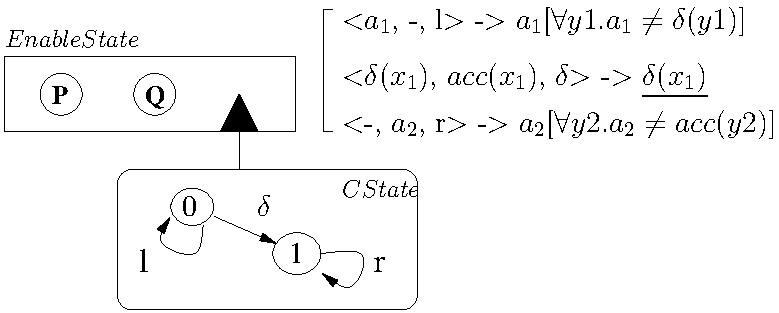
\includegraphics[width=\linewidth]{ActaXFIG/Enable1}
  \\[1.3ex]
 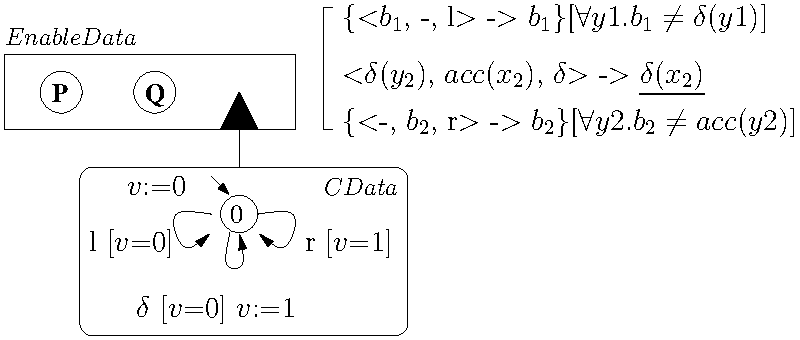
\includegraphics[width=\linewidth]{ActaXFIG/Enable2}
  \caption{Two pNet encodings for  Enable }  \label{schema:enable-pnets}
\end{minipage}
  \hspace{2mm}
\begin{minipage}{6cm}
  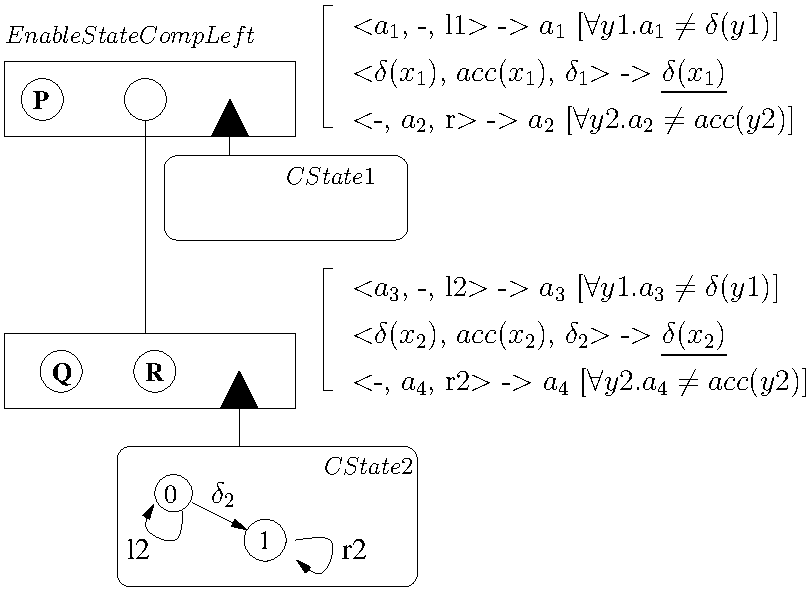
\includegraphics[width=\linewidth]{ActaXFIG/P-QR}
  \caption{Composed pNet for ``$P>>(Q>>R)$''}  \label{schema:enable-composed}
\end{minipage}

\end{figure}

	To give an intuition of the open pNet model and its semantics, we use
	here a simple example based on the ``Enable'' operator of the LOTOS language.
	In the Enable expression ``$P>>Q$'', an \texttt{exit} statement within $P$
	terminates the current process, carrying a value $x$ that
	is captured by the \texttt{accept} statement of $Q$. 	
	We use a simple action algebra,
	containing two constructors $\delta(x)$ and $acc(x)$, for any
	possible data type of the variable $x$, corresponding to the
	statements \texttt{exit} and \texttt{accept}. 
	We need no specific predicate over the action expressions, apart
	from equality of actions.
        
	In Figure \ref{schema:enable-pnets}, we show two possible encodings of the  
	``Enable'' operator.
        In the first encoding $EnableState$, in the upper part of
	Figure \ref{schema:enable-pnets}, we use a controller $CState$ with two
	states, and simple control actions $l, r, \delta$. The second encoding
	$EnableData$ uses a data-oriented style, with a single state controller $CData$, and a
	state-variable $v$, with values in $\{0,1\}$.

        In this example we use \emph{synchronised
          actions}, to express actions that cannot be further synchronised, similar to the
         silent action $\tau$ of CCS. We denote them as any action expression with the text
        underlined, as e.g. $\underline{\delta(x_2)}$. Such
        synchronised actions do not play any special role for defining
        the semantics of pNets, but as one can expect, will be crucial
        for defining weak equivalences.
	
	Note that synchronisation vectors are defined in a parameterised
	manner:  the first and third lines represent one vector
	for each possible action of hole $P$
	(resp. $Q$). This notation can also use predicates, as in the first
	case, in which we want the vector to apply to any action of $P$
	except for $\delta(z)$.
	
	In Figure \ref{schema:enable-composed}, we enrich our example by
	composing two occurences of the $EnableState$ pNet. In Section
        \ref{section:use-case:Enable} we will show how these encodings can
        be used to prove properties of the Enable operator.




\section{Operational Semantics of Open pNets}
\label{section:op-semantics}

The semantics of an open pNet will be defined as an open automaton, which
is an automaton where each transition represents the composition transitions 
of several
% \noteSB{These should all be PLTSs, right? Or did I miss
%  something?}\noteEM{Hum, nor really, something intermediate; the actions there can be
%  parameterised actions, but the label has no guard and no
%  assignments}
LTSs with the actions of some holes; a transition occurs if its predicates hold,
and can involve a set of state modifications. Each state of an open
automaton has a set of \emph{state variables} that can be assigned by
incoming transitions.
%Strictly speaking, the LTSs at the leaves of the
%open automaton are a restricted form of PLTSs, where labels are
%parametrised actions, but include no guard nor assignments.


\begin{definition}[Open transitions]
	\label{def:OpenTransitions}
	An \emph{open transition} ($OT$) over
	% a set  $\langle S_i,s_{0 i}, \rightarrow_i\rangle^{i\in I}$ of LTSs,
	a set $J$ of holes %with sorts $Sort_j^{j\in J}$
	and a set of states $\mathcal{S}$ is a structure of the form:	
	\begin{mathpar}
		\inferrule*[myfraction=\reddottedrule]
		{%\{s_i~{\xrightarrow{a_i}}_i ~s_i^{\prime}\}^{i\in I},
			\{\xrightarrow{\beta_j}_j\}^{j\in J}, \Pred\,, \Post}
		{s \xrightarrow {\alpha}s'}\,,
	\end{mathpar}
	where $s, s'\in\mathcal{S}$, the $\beta_j, \alpha$ are
        action expressions,
        % $s_i{\xrightarrow{a_i}}_i s_i^{\prime}$ is a transition of the 
	% LTS $\langle S_i,s_{0 i}, \rightarrow_i\rangle$
	$\beta_j$
	is an action of the hole $j$, and $\alpha$ is the resulting action
	of the $OT$. \Pred\ is a predicate
	over the variables of the terms, labels, and states $s_i$,
	$\beta_j$, $s$, $\alpha$. \Post\ is a set of equations that  
	hold \emph{after the open transition}, represented as a
	substitution $\{x_k\gets e_k\}^{k\in K}$  
	where $x_k$ is a variable of $s'$ or $s'_i$, whereas $e_k$ is an
	expression over other variables of the open transition.
\end{definition}


\begin{definition}[Open automaton]
	\label{def:open-automaton}
	An \emph{open automaton} is a tuple $
	\langle I, J,\mathcal{S},s_0,\mathcal{T}\rangle$, where
	\begin{itemize}
		\item[$\bullet$]  $I$ and $J$ are  two sets of indices,
		%	\item[$\bullet$]  $LTS_i^{i\in I}$ is a family of LTSs,
		\item[$\bullet$]  $\mathcal{S}$ is a set of states and $s_0 \in \mathcal{S}$ the initial state,
		\item[$\bullet$] $\mathcal{T}$ is a set of open transitions and, for each
		$t\in \mathcal{T}$, there exist $I'$, $J'$ with $I'\subseteq I$, $J'
		\subseteq J$, such that $t$ is an open transition over $J'$
		and  $\mathcal{S}$.
		
	\end{itemize}
\end{definition}
%
%Then the semantics of a pNet is characterized by a set of {\em open
%transitions}, where the hypotheses on process parameters are
%replaced by 1) transitions of the PLTSs at the leaves, and 2) formal
%hypotheses on the transitions of the holes. A {\em predicate} is used
%to relate the parameters and names appearing in the actions of the
%leaves and the holes involved in the rules, but also appearing in  the resulting action.

The \emph{states} and the shape of \emph{predicates} in the
transitions
of an open automaton representing the semantics of a pNet
have the following specific structure.

\paragraph{States of open pNets.}\label{def-states}
A state of an open pNet is a tuple of the
states of its leaves. We denote tuples
in structured states in the form $\triangleleft\ldots\triangleright$.
For any pNet $p$, let $\langle S_i,{s_i}_0, \to_i\rangle^{i \in L}$ be the set of PLTSs at its leaves,
then $\mathit{States}(p) = \{\ostate{s_i^{i\in L}}
|\, \forall i\in L. s_i \in S_i\}$.
A PLTS could be its own single leave:
$\mathit{States}(\langle S,s_0, \to\rangle) = \{\ostate{s}|\, s \in S\}$.
The initial state is defined as:
$\mathit{InitState}(p) = \ostate{{{s_i}_0}^{i\in L}}$.


%% \begin{example} \emph{State of a pNet}
%%   The states of pNet \texttt{EnableCompL} are:
%%   $\triangleleft 00 \triangleright, \triangleleft 10 \triangleright, \triangleleft 11 \triangleright$
%% \end{example}

\paragraph{Predicates.}
Let
$\langle\overline{\pNet},J,\symb{SV}_k^{k\in K} \rangle$
be a pNet. Consider a synchronisation vector $SV_k$, for $k\in K$. We build a
predicate $\MkPred$ relating
the actions of the involved sub-pNets and the resulting actions. This predicate verifies:
\begin{multline*}
	\MkPred(SV_k, a_i^{i\in I}, b_j^{j\in J}, v)\Longleftrightarrow
	%% \begin{array}{l}
	\exists {(a'_i)}^{i\in I},
	{(b'_j)}^{j\in J},v'.\\
	SV_k={(a'_i)}^{i\in I}, {(b'_j)}^{j\in J}\rightarrow v'
	\land
	\forall i\in I.\, a_i=a'_i\land \forall j \in J.\, b_j=b'_j \land v=v' . 
\end{multline*}

%% \end{array}


%% This definition is not constructive but it is easy to build the
%% predicate constructively by brute-force unification of the sub-pNets
%% actions with the corresponding vector actions, possibly followed by a simplification
%% step. 

\begin{example}[Open transitions]
  Transition $OT_2$ of the pNet $EnableStateCompLeft$ is generated by
  combining the first vector of its root node with
  the second vector of its second node. The global states show that
  controler $CState1$ is 
  changing from state 0 to 1.
  \label{OT:example-1}
        \begin{mathpar}
	  OT_2  =
          \inferrule*[myfraction=\reddottedrule]
	{\{\xrightarrow{\delta(x2)}_P ~~
          \xrightarrow{acc(x2)}_Q \} ~~
          [\forall z. acc(x2) \neq \delta(y1)]
        }
	{\ostate{0,0} \xrightarrow {\underline{\delta(x2)}} \ostate{1,0}}
	\end{mathpar}

If we use the data-oriented pNet $EnableData$ from Figure
\ref{schema:enable-pnets} to build a similar $EnableDataCompLeft$  expression
``$P>>(Q>>R)$'', the corresponding open transition would be:

  \label{OT:example-2}
        \begin{mathpar}
	  OT_2'  =
          \inferrule*[myfraction=\reddottedrule]
	{\{\xrightarrow{\delta(x2)}_P ~~
          \xrightarrow{acc(x2)}_Q \} ~~
          [v_1=0 \land v_2 = 0 \land \forall z. acc(x2) \neq
            \delta(z)] ~~ \{v1:=1\}
        }
	{\ostate{0,0} \xrightarrow {\underline{\delta(x2)}} \ostate{0,0}}
	\end{mathpar}
        where $v_1$ and $v_2$ are respectively the state variables of
        the first and second $EnableData$ pNets. Indeed the global
        state space of this version is reduced to $\ostate{0,0}$, and
        the state change is replaced by the assignment ``$v_1:=1$''.
        
\end{example}


\paragraph{Structural Semantic Rules.}
The semantics of pNets in terms of open automata has been defined in
\cite{henrio:Forte2016}, in the form of two structural rules, one for
PLTSs, and the other for pNet nodes. These rules are slightly improved, adding guards in the synchronisation vectors and syntax for universal quantifier in the guards (see~\cite{Avocs-RR})\footnote{For convenience, we provide these rules and the proof of the finiteness theorem in Appendix~\ref{appendix:semRules}}. 
  
In \cite{henrio:Forte2016} we also proved the following result, which
ensures the termination of our semantic construction algorithm.
\begin{theorem}[Finiteness]
  \label{Th:finiteness}
   Let $pnet=\langle \overline{\pNet},\overline{S}, \symb{SV}_k^{k\in K}\rangle$ be an open pNet  with leaves $l_i^{i\in I}$ and holes $h_j^{j\in
 	J}$, where the sets $I$ and $J$ are finite. Suppose the synchronisation vectors of all pNets 
 included in  $pnet$   are finite, and 
 % $\forall i \in L.\, finite{(states(l_i))} \text{ and } l_i$ 
 $l_i $ has a finite number of state variables for each $i\in I$. Then the semantics of $pnet$ is an open automaton 
 %$\mathcal{T}$ 
 with finitely many states and transitions.
\end{theorem}
Notice that all the elements of such pNets and open automata are symbolic, and they can represent many classes of unbounded systems. 


\section{Generation of Open Automata}
\label{section:implementation}
In this section we describe an algorithm implementing the pNet
semantics, its new ``on-the-fly'' version, and the interaction with the
Z3 SMT solver. Under the hypotheses of Theorem \ref{Th:finiteness} 
both algorithms terminate. 

%% \noteSB{
%% line 11: Would it not be better to prune unsatisfiable transitions
%% on-the-fly, \ie inside the loop?}
%% \noteEM{Not so easy, it would require a proof... on one side this
%%   would implement reachability on the fly; but there is the question
%%   of collecting the assignments of the state variables, that are used
%%   in the sat check !}

\begin{algorithm}[h]
  \caption{Open Automaton Generation}
  \label{alg1}
\begin{algorithmic}[1]
\Require A pNet $P$ (can be a PLTS, but not a hole)
        %\qquad \hl{\textbackslash\textbackslash~SB: was `` pn ''}
\State Initialize sets $U=\{\mathit{InitState}(P)\}$ and $E=\emptyset$,
for unexplored and explored global states, respectively; $L=\emptyset$ for the resulting OTs;
\While{!$\mathit{isEmpty}(U)$}
	\State Choose $S$ in $U$; remove $S$ from $U$, add $S$ to $E$;
        %\qquad \hl{\textbackslash\textbackslash~SB: was `` Choose $S$ in $U$ ''}
	\State $\mathit{OTs} = \mathit{MakeTransitions}(P, S)$;
	\For {each $\mathit{OT} \in \mathit{OTs}$}
          \State Add $\mathit{OT}$ to $L$;
          \State Let $S'$ be the target state of $\mathit{OT}$;
          add $S'$ to the unexplored states if necessary:
	  \IfThen{($S' \not\in U \cup E$)}{Add $S'$ into $U$;}
	  \EndFor
\EndWhile
\State $\mathit{L1}$=\textit{filterUnsatTransitions}($\mathit{L,Assignments}$);
\State $\mathit{OA_1^0}$=\textit{makeReachableSubAutomaton}($\mathit{InitState}(P),L1)$;
\Repeat $\mathit{OA_1^n}$=\textit{RefineReachableSubAutomaton}($\mathit{OA_1^{n-1}}$)
\Until  $\mathit{OA_1^n}=\mathit{OA_1^{n-1}}$;   \hfill $\setminus \setminus$ Fixed point reached
\State \Return $\mathit{OA_1^n}$;

\end{algorithmic}  
\end{algorithm}

Algorithm~\ref{alg1} starts with an open pNet and builds its set of open
transitions. Its main loop is a classical residual algorithm: starting
from the initial global state, it picks a state in an unexplored set, 
computes all possible OTs, and adds the target states in the
unexplored set, until this set is empty.

The inside loop (\emph{MakeTransitions} method) applies recursively
the semantic rules following the structure of the pNet.
When applying a rule to a PLTS at the leaves, we simply take the PLTS transitions of the
corresponding local state and use the semantic rules to build the OT.
When applying a rule to a pNet node we use two methods, \emph{combining} and
\emph{matching}, to generate the open transitions in a hierarchical manner,
as shown in Algorithm~\ref{alg2}. This method directly manages the
holes of the node, so \emph{MakeTransitions} is never called on a hole.

Before the SAT checking step, the set $L$ may contain symbolic transitions that
do not have valid ground instantiations. This is not logically
incorrect, but is naturally not an optimal representation. So (line 11) we prune
these UNSAT transitions: at the end of the open automaton generation,
the predicate of each OT is translated 
into SMTlib assertions (see Section~\ref{section:pruning}), and then checked for
satisfiability (function \textit{filterUnsatTransitions}). 
Then we compute (lines 12-14) the set of reachable transitions and states to build
the final open automaton (more details in Section~\ref{section:BuildingTheOpenAutomaton}).


\begin{algorithm}[h]
\caption{MakeTransitions() \em{for a pNet node}}
  \label{alg2}
\begin{algorithmic}[1]
\Require a pNet node $P$ with subnets $\overline{sn}$ and holes $\overline{hole}$; a global state $S$.
\State Initialize empty list $l$ and set $L$ for sub-transitions and transitions, respectively;
	\For{each $\mathit{Subnet}$ in $\overline{sn}$}
        \hfill $\setminus \setminus$ Recursively apply the semantic rules on the subnets
           \State Store $\mathit{MakeTransitions}(Subnet, S)$ in $l$;
	\EndFor
	\State $\overline{comb} = \mathit{Combining}(l)$;
	\For{ each $sv \in SV$ and each $comb \in \overline{comb}$ }
           \State $ot = \mathit{Matching}(sv, \overline{\mathit{comb}}, \overline{\mathit{hole}})$;
           \IfThen{($ot$ is defined)}{Store $ot$ in $L$; ~~~ $\setminus \setminus$ if $\mathit{Matching}()$ succeeds}
	\EndFor
\State \Return $L$;
\end{algorithmic}  
\end{algorithm}



%
%For holes, their behaviour is unspecified, it doesn't have an exact
%external presentation of action. We only give an action variable to each hole
%and treat it as hole behaviour to suppose working status of the
%hole.
%% Here should have a constraint that this variable belongs to the sort of hole.
%In every case, the hole behaviours are unchanged, so we
%only make the combinations of subnets' open transitions. 
%


\def\inactive{\{-\}}
\paragraph{Combining.}
The combining method enumerates all the possible behaviours of the
subnets as all the possible combinations of their open transitions.
Assume that there is a collection of $n$ subnets.
%% \noteSB{These variables are not used and conflict with the returned
%%   set $L$ in Alg.~\ref{alg2}, on one hand, and control states $s_i$ of
%%   the subnets, on the other.}
%% \st{$L = {s_1, s_2, ...,  s_n}$;}
We denote by $\overline{ot}_i$ the set of open
transitions of the $i$-th
subnet (obtained in line~3 of the algorithm); %% $s_i$ and 
``$-$'' means that the subnet is not involved.
The combination $\overline{comb}$, a set of $n$-tuples, is the
cartesian product:  
$$\overline{comb} = (\inactive\cup \overline{ot}_1) \times (\inactive\cup \overline{ot}_2)\times \dots \times (\inactive\cup \overline{ot}_n). $$

%Algorithm 2 shows the combining algorithm for enumerating all possible
%working status combinations from subnets. Dealing with a list $TR$
%containing  sets of open transitions from different subnets,
%the algorithm choses one of sets $L_{ot}$ and does combining on the
%remaining part of $TR$ recursively. The case when a subnet is not working is
%managed by adding a $null$ into the $L_{ot}$.



\paragraph{Matching.}
The \emph{Matching} method builds the OTs of a pNet node from those of
its subnets.
For each synchronisation vector and each possible
combination of behaviours of the subnets, as generated by the \emph
{Combining} method, it builds the corresponding open transition.
Here, we only detail the construction of the predicate.
Suppose that $sv = \left((a'_i)^{i\in I} (b'_j)^{j\in J}\rightarrow v'\right) \in SV$ is a synchronisation vector, $G_k$ is its guard, and
$C = ({ot}_i)^{i \in [1,n]} \in \overline{comb}$ is a tuple of open transitions such that, for each $i \in [1,n]$, either $ot_i = -$, or the result action of $ot_i$ is $a_i$. Suppose futher that $\mathit{hole} = (b_j)^{j \in J}$ is the hole behaviour and $v$ is a fresh variable, representing the result action of the OT under construction. Then we can  build the predicate:
%
\begin{multline*}
  \mathit{MkPred}(sv, C, \overline{\mathit{hole}}) = 
  (\forall i\in I, a_i=a'_i) \land
%  (\forall i \not\in I, ot_i = -) \land
  (\forall j\in J, b_j=b'_j) \land
  (v=v') \land G_k.
\end{multline*}


\paragraph{Filtering.}
While matching a vector with a combination tuple, \emph{Matching}
tries to filter out some incompatibilities; there may be several
reasons why the matching would fail: 
\begin{itemize}
  \item if some subnet is marked as inactive in the vector, and the
    chosen combination has an active behaviour at this position, or vice-versa;
  \item if some subnet action expression in the vector does not match (by
    pattern-matching) with the corresponding action expression in $C$;
  \item or if the whole set of active subnet actions in the vector
    cannot be matched (by unification) with the corresponding action expressions
      in the tuple $C$ (this is strictly stronger than the
      previous filter). 
\end {itemize}

Even when unification succeeds, it is still possible that
the resulting predicate would be unsatisfiable, because of some
incompatibility involving the guards. In our algorithm, we choose to
apply only the simplest filter inside the \emph{Matching} method
(before applying the predicate and OT construction). Matching and
unification  will be checked later, together with the guards collected
from synchronisation vectors and from PLTS transtions, using the
satisfiability check in the SMT engine.


\subsection{Management of State Variables and Assignments}


In a PLTS, there may be several incoming transitions 
that assign potentially different (symbolic) values to a state variable.
To handle such cases, the algorithm manages a
list of assignment expressions for each PLTS state. 
The only assignments for state variables that happen at the PLTS level
are as follows: every time the $MakeTransitions$ method 
 is applied on a PLTS, it collects the expressions from the
$Post$ in each transition. 
% As there is no assignments collecting work on a pNet node, it is not
% shown in Algorithm~\ref{alg2}.

For a global state in the open automaton, the set of state
variables (which may be used in an outgoing transition) 
is the disjoint union
of the sets of state variables of the individual PLTS states constituting this
global state. The final assignment sets are assembled when building the
open automaton from the reachable transitions, see below.


%% \QIN{
%% The list we used contains several triples <$v$, $S$, $AssignRH$> to
%% record the information of both state and global variables of the PLTS,
%% where $v$ is the variable in PLTS, $S$ is its owner state and
%% $AssignRH$ is a list of expressions over other variables in the right
%% hand side of assignments of $v$. It means the variable is global in
%% the PLTS belonging to all the states, if $S$ is $null$. We update the
%% list of record triples every time Tr1 is applied. Then we can track
%% all the possible (symbolic) value of the variables when computing open transitions.
%% }

\subsection{Pruning the Unsatisfiable Results}
\label{section:pruning}



Our matching/filtering strategy builds some transitions where
the predicates express incompatible constraints. Even if having an
unsatisfiable (symbolic) transition would not be incorrect,
we choose to minimize the open automaton (\ie its number of
transitions and states), by checking the predicates for satisfiability.

\begin{example}[Unsat OT]
  \label{schema:unsat-ot}
\begin{mathpar}
	  OT_{19}  =
          \inferrule*[myfraction=\reddottedrule]
	{\{\xrightarrow{a1}_P ~~
          \xrightarrow{acc(x2)}_R \} ~~
          [a1 = \delta(x2) \land \forall z. a1 \neq \delta(z)]
        }
	{\ostate{2,0} \xrightarrow {\underline{\delta(x2)}} \ostate{3,0}}
	\end{mathpar}

Here we display an  
unsatisfiable open transition 
from the open automaton of our running example.
It shows the case where processes $P$ and $R$ ``try'' to communicate directly, but this is made impossible by the combination of chosen synchronisation vectors and their guards. This
  mismatch is materialised by the predicate
fragment ``$a1 = \delta(x2) \land \forall z. a1 \neq \delta(z)$''. In Section~\ref{section:TranslationToSMTlib} we will show how this is encoded and checked using the SMT engine.
\end{example}



Checking satisfiability requires some symbolic computation
on the action expressions and the predicates, which
may depend on the specific theory of the action algebra datatypes. 
The ``Modulo Theory'' part of SMT solvers is important here, as
the solvers can use specific properties of each data type in the action algebra.

In Algorithm~\ref{alg1}, functions \textit{filterUnsatTransitions} (in line 11) 
\textit{RefineReachableSubAutomaton} (in line 13) make use of the Z3 engine to implement the
satisfiability checking, for all the OTs computed that far.
For a transition
\[		\inferrule*[myfraction=\reddottedrule]
		{%\{s_i~{\xrightarrow{a_i}}_i ~s_i^{\prime}\}^{i\in I},
			\{\xrightarrow{\beta_j}_j\}^{j\in J}, \Pred\,, \Post}
		{s \xrightarrow {\alpha}s'}
                \]
                we need to build a predicate encoding both the OT predicate and
the information available on the possible assignments of the initial
state $s$. This is expressed as
\[Pred_{l}\wedge \bigwedge_{v\in vars(s)}\{ \bigvee_{Assign\in
  assigns(v,s)} Assign\}
\]
where each $Assign$ represents one of the possible (symbolic) value of
 the state variable $v$.

\subsection{Building the Open Automaton}
\label{section:BuildingTheOpenAutomaton}

The set $L1$ may contain unreachable transitions. To remove those
transitions, the last step of the  
algorithm (lines 12-14) builds the final open automaton via a traversal of $L1$,
starting at the initial state $InitState(p)$ as defined in
page~\pageref{def-states}. More precisely, this is a residual
algorithm building a graph from the reachable transitions in $L1$. 
%and states are the set of target states of the transitions. 
Each state in the graph is decorated with a set of its local
variables, and a list of their possible assignments,
gathered during the traversal using the ``Post'' parts of the
OTs.

A further reduction may now be gained by using the information from
these sets of possible assignments: adding this information when
checking satisfiability of transitions leaving a given state may
result in more UNSAT transitions. The set of possible
assignments computed by the algorithm is an over approximation of
possible values of the 
variables of such state, so narrowing it means we get a better
approximation, and potentially more information, which can be used in
the SAT checking of subsequent transitions. In turn, this may reduce the possible
assignments of the corresponding target states. In
Algorithm~\ref{alg1}, we iterate this procedure (lines 13-14), each iteration
reducing the set of 
transitions and the sets of assignments; the final open automaton
is the fixed point of this iteration.

In practice, this could be
expensive, and it is not incorrect to leave some UNSAT OTs in the
result. From a  practical point of view, very little will be gained to compute the
fixed point, so we would only perform one step of iteration. Further algorithms 
(e.g. model-checking or equivalence checking) will be able to use the
full information from the predicates and the assignment sets, even if
some spurious OTs are left here.

\subsection{Computing Reachable State Space on the Fly}

The basic algorithm introduced above potentially explores some
areas of the global state space that will not be reachable after
checking the OTs' predicates for satisfiability. Incorporating the
satisfiability check inside the residual algorithm will definitely
save some of these useless computation. More precisely, it will still
create, and submit to Z3, the OTs at the ``border'' of the state space, but
not the transitions issued from non-reachable global states. We use
this idea to create our ``smart'' algorithm.

But there is more to this. Due to the symbolic nature of the
  transitions, reachability is not as easy to define as in standard
  models, as illustrated by the discussion above. By avoiding building
  the OTs coming from some unreachable states, we also avoid adding
  the corresponding assignments to the variables of their target states.
But we \emph{cannot} use the
assignment information in the ``on-the-fly'' SAT checking, because
they cannot be complete before exploring (at least) all the reachable
state space. We first need to compute an over-approximation of
the reachable state space and assignment sets; this corresponds to
the automaton $OA_2^0$ in Algorithm~\ref{alg3}, line 13.
So the smart algorithm proceeds in two steps: during the
first step, the SAT checking is done without using any assignment set
information (line 5).  Only the OTs found SAT from this check will be added
to $L$, and the corresponding target global state added to $U$ if
necessary. This ensures that all explored global states are
effectively reachable by a chain of SAT OTs.
 
\begin{algorithm}[h]
  \caption{``Smart'' Reachable Open Automaton Generation}
  \label{alg3}
\begin{algorithmic}[1]
\Require A pNet $P$ (cannot be a hole)
        %\qquad \hl{\textbackslash\textbackslash~SB: was `` pn ''}
\State Initialize sets $U=\{\mathit{InitState}(P)\}$ and $E=\emptyset$,
for unexplored and explored global states, respectively; $L=\emptyset$ for the resulting OTs;
\While{!$\mathit{isEmpty}(U)$}
	\State Choose $S$ in $U$; remove $S$ from $U$, add $S$ to $E$;
        %\qquad \hl{\textbackslash\textbackslash~SB: was `` Choose $S$ in $U$ ''}
	\State $\mathit{OTs} = \mathit{MakeTransitions}(P, S)$;
	\For {each $\mathit{OT} \in \mathit{OTs}$}
        Check satisfiability of $\mathit{OT}$ using the SMT solver;
        \IfThen {$SAT(\mathit{OT})$}
                {\State \{Add $\mathit{OT}$ to $L$;
                  \State Let $S'$ be the target global state of $\mathit{OT}$
	          \IfThen{($S' \not\in U \cup E$)}{Add $S'$ into $U$;}
                  \}}
	\EndFor
\EndWhile
\State $\mathit{L2}$=filterUnsatTransitions($\mathit{L,Assignments}$);
\State $\mathit{OA_2^0}$=makeReachableSubAutomaton($\mathit{InitState}(P),L2)$;
\Repeat $\mathit{OA_2^n}$=RefineReachableSubAutomaton($\mathit{OA_2^{n-1}}$)
\Until  $\mathit{OA_2^n}=\mathit{OA_2^{n-1}}$;
\State \Return $\mathit{OA_2^n}$;
%\EndIf
\end{algorithmic}  
\end{algorithm}



At the end of the residual loop, we do another traversal of the
automaton, this time using the assignment information collected that
far (line 12), and compute the final reachable sub-automaton
iteratively (lines 13-15), in the same way as in Algorithm \ref{alg1}. 
Naturally, this step is only useful if there are some assignments.

\medskip
Now we will prove that the smart algorithm computes essentially the same 
open automata as those of the original algorithm.

The easy case is when the system does not contain assignments to state
variables. This does not mean ``data-independency'': we can still have
guards in the PLTS transitions and in the synchronisation vectors,
making the behaviour depending on the values of input variables. But
the open automaton needs not to collect the set of possible values dealing
with the values of local variables, so the final automaton is $AO_2^0$ as
computed in line 13.

\begin{theorem}[Correctness without assignments]
  \label{Th:CorrectnessWithoutAssignments}
For a pNet satisfying the finiteness conditions of Theorem~\ref{Th:finiteness} and
containing no assignment to state variables, the smart  
algorithm, without a final reachability computation, computes 
the same open automaton as that of Algorithm~\ref{alg1} up to a renaming of
variables in the transition labels.  
  \end{theorem}

\begin{proof} %[Theorem \ref{Th:CorrectnessWithoutAssignments}]

 Let $pn$ be a pNet. The set of states 
 managed by the two algorithms both are subsets of the cartesian
 product of the PLTS states, as defined in page \pageref{def-states}. In a
 similar way, the set of state variables attached to each state are
 also equal. Comparing  
 transitions requires a little more care, because within the
 $MakeTransitions$ function, fresh variables are created everytime a
 synchronisation vector is used (this occurs within the $MkPred$ and
 $matching$ functions). However, given a global state, the call of
 $MakeTransitions$ will always return exactly the same set of OTs, up to a
renaming of these fresh variables. When this is not ambiguous, we will
speak of equality (of transitions, and of open automata) without the phrase ``up to a renaming of fresh variables''.

  Let us first define some notations.
 \begin{itemize}
    \item $L0$: the original set of transitions by Algorithm~\ref{alg1}
      (i.e. before line 11), 
    \item $L1_{sat}$:  the original set of transitions by Algorithm~\ref{alg1}, after
      satisfiability check (i.e. after line 11),
    \item $L1_{reach}$: the final set of OTs of Algorithm~\ref{alg1}, as computed
      by line 12 (as $OA_1^0$). 
      %Without assignments the following
      %refinement step will do nothing, the fixpoint is already reached.
    \item $L2_{sat}$: the original set of transitions by Algorithm~\ref{alg3}
      (i.e. before line 13), 
    \item $L2_{reach}$: the final set of OTs of Algorithm~\ref{alg3}, as computed
          by line 13. Here also $OA_2^n = OA_2^0$.
   \item $States: \overline{OT}\rightarrow\overline{State}$:  the function that
computes the set of target states of a set of OTs.  
  \item $Rename:  L1_{reach} \rightarrow L2_{reach}$:  a function that
    keeps state names of transitions but renames fresh variables in
    the transition labels. In the sequel, transitions $l_i$ will range
    over $L0$ set (and $L1_*$), and $l'_i$ will range over $L2_*$
    sets. Of course renaming preserves satisfiability.
\end{itemize}

\smallskip
We now prove that $L1_{reach}=L2_{reach}$ and
$States(L1_{reach})=States(L2_{reach})$.

By definition of the algorithms, we have:

\centerline{$L1_{reach} \subseteq L1_{sat} \subseteq L0$ \qquad \mbox{and}\qquad
$L2_{reach}\subseteq  L2_{sat}$\ .}
%\centerline{$L2_{reach}\subseteq  L2_{sat}$}

\smallskip
Let $S=\ostate{\overline{s}}=\ostate{\{s_{i}\}^{i\in Leaves(pn)}}$
range over the global states $States(L0)$, 
The only difference between the main loops of the algorithms is that 
Algorithm~\ref{alg3} only retains the satisfiable OTs (lines 6-7), so 
Algorithm~\ref{alg3} computes fewer transitions than
Algorithm~\ref{alg1}. Formally, we have that
$L2_{sat} \subseteq Rename(L0)$ (up to a renaming of fresh variables), and as a consequence $States(L2_{reach})\subseteq  States(L0)$, i.e.,\\
\centerline{$\forall \ostate{\overline{u}}\in States(L2_{reach}), \exists\ostate{\overline{t}}\in States(L0), \ostate{\overline{t}}=\ostate{\overline{u}}$\ .}

For a global state $S$, and a set of OTs $L$, define its distance
$|S|_L$ as the length $n$ of (one of the) shortest chain
$S_0\xrightarrow{l_1}S_1\xrightarrow{l_2}...S_{n-1}\xrightarrow{l_{n}}S$
  from the initial state $S_0$, with $l_k \in L$ for each $k\in [1..n]$.

\medskip
We will prove by induction on the distance from the original state
that\linebreak $\forall S \in L0. \forall n \in \mathbb{N}. S \in States(L2_{reach}) \land |S|_{L2_{reach}}=n \Rightarrow S
\in States(L1_{reach})$, and vice-versa.

  The initial property is trivial, for $n=0$, both state sets of
  distance zero are reduced to $\{S_0\}$.

  Suppose our property is true for distance $n$, and
  suppose $|S|_{L2_{reach}}=n+1$, then there exists a chain
  $S_0\xrightarrow{l'_1}S_1\xrightarrow{l'_2}...S_{n}\xrightarrow{l'_{n+1}}S$
  with all $l'_k \in L2_{reach}$. In particular, since
  $L2_{reach}\subseteq L2_{sat}$, we have that $l'_{n+1} \in L2_{sat}$ and
  its predicate is satisfiable.
  
  By induction hypothesis, we get $S_{n} \in States(L1_{reach})$, so during the
  call of $makeReachableSubAutomaton$ in Algorithm~\ref{alg1}, line
  12, there exists an OT
  $S_n \xrightarrow{l_{n+1}}S$ in $L1_{sat}$, with $l'_{n+1}=Rename(l_{n+1})$;
  this OT will be checked and found SAT, so
  $S \in States(L1_{reach})$. 

  Conversely, if $|S|_{L1_{reach}}=n+1$, we get a similar chain in
  $L1_{reach}$, with the transition $S_n \xrightarrow{l_{n+1}}S$.  Then $ S_n \in
  States(L1_{reach})$ and $l_{n+1}$ is satisfiable. By induction, we have
  $S_n \in States(L2_{reach})=States(L2_{sat})$, so there exists
  $l'_{n+1}=Rename(l_{n+1})$ that will have
  been checked on the fly, in line 6 of Algorithm~\ref{alg3}. Then
  the transition $S_n \xrightarrow{l'_{n+1}}S$ will be added to
  $L2_{sat}$, and thus $S \in States(L2_{reach})$. 
  
Note that $L0$ is finite. Therefore, we can conclude that $L1_{reach}=L2_{reach}$ and
$States(L1_{reach})=States(L2_{reach})$. 
\hfill\qed
\end{proof}

\paragraph{General case with assignments.}
In the presence of assignments, we need to collect all of them
  before using the assignment information to refine the SAT
  checking. Still, the smart strategy will explore a reduced state
  space, though not necessarily the minimal one. In the
  following theorem, both algorithms are considered in their complete
  version, meaning the reachability (with assignments) step is
  iterated up to fixed points.
  
\begin{theorem}[Correctness with assignments]
  \label{Th:CorrectnessWithAssignments}
In the general case, if a pNet satisfies the finiteness conditions of Theorem~\ref{Th:finiteness} and contains some assignments to state variables, the smart algorithm computes 
the same open automaton as that of Algorithm~\ref{alg1} up to a renaming of variables in the transition labels.
\end{theorem}

%\TODO{Formalize the proof}
\begin{proof}
  Define the OT sets $L0, L1_{sat}, L2_{sat}, L2_{reach}$ and the
  function $States$ as before, and: 

  \begin{itemize}
    \item $L_1^*$: the final set of OTs of Algorithm~\ref{alg1}, as computed
        by an iterative application of $makeReachableSubAutomaton$ (line
        14) up to a  fixed point.
    \item $L_2^*$: the final set of OTs of Algorithm~\ref{alg3}, as computed
        by an iterative application of $makeReachableSubAutomaton$ (line
        15) up to a fixed point.
    \item $Assigns : \overline{OT}\ \rightarrow \overline{Assign}$: the function
          of computing the set of assignments of (the variables of the
          states of) a given set of OTs.
    \item $AssignsVar : Vars\times\overline{OT} \rightarrow \overline{Assign}$: the function of computing the set of assignments of a specific state variable in a transition.
  \end{itemize}

%?? In Theorem 2, we have already proved that the result automata $OA_1$ and $OA_2$ of the two algorithms are the same if the pNet contains no assignment to its state variables.

\smallskip
The structure implicitly computed by both algorithms is a triple
$Aut= \langle \overline{OT},\overline{State},\\ \overline{Assign}\rangle$.

We already know that $L2_{sat}\subseteq L1_{sat}$ (up to a renaming),
because every OT that will be checked positively (using assignments) in line 12 of
Algorithm \ref{alg3} will also be tested in Algorithm \ref{alg1} (as
$L2_{sat}\subseteq L0$), and with a larger set of assignments.

Consequently, the initial triples of the refinement loop are:
\begin{align*}
Aut_1^0 = \langle L1_{sat}, States(L1_{sat}), Assigns(L1_{sat})\rangle \\
Aut_2^0 = \langle L2_{sat}, States(L2_{sat}), Assigns(L2_{sat})\rangle \\
\text{with } Aut_2^0 \subseteq Aut_1^0, \text{ component-wise and up to a renaming.}
\end{align*}

%% The assignments set of $OA_1^0$ is $\{Assigns(L1, States(L1))\}$ and
%% that of $OA_2^0$ is $\{Assigns(L2_{sat}, States(L2_{sat}))}\}$. The
%%   result triples are:    
%% \noindent
%% \begin{align*}
%% Aut_1 = \langle L1_{sat}, States(L1_{sat}), \{Assignments(L1, S_i)\}^{S_i\in States(L1)}\rangle\ , \\
%% Aut_2 = \langle L2_{sat}, States(L2_{sat}), \{Assignments(L2_{sat}, S_j)\}^{S_j\in States(L2_{sat})}\rangle \  .
%% \end{align*}

Based on each triple structure $Aut$, we define the function $Refine : Aut
\rightarrow Aut$ modelling the function $makeReachableSubAutomaton(S0,OTs)$. It
uses the assignments of the OTs remaining from the previous iteration
to refine the computed reachable space: 
\begin{align*}
Aut^n = Refine(Aut^{n-1}) &=\langle L^n, States(L^n), Assigns(L^n)\rangle
\end{align*}
where $L^n = Reach(L^{n-1} - L^{n-1}_{unsat})$, and $L^{n-1}_{unsat}$ is the
set of unsatisfiable transitions checked in this iteration. We have
$L^n\subseteq L^{n-1}$, and consequently, their states and assignments
may be reduced:
$$States(L^n)\subseteq States(L^{n-1}) \land Assigns(L^n)\subseteq
Assigns(L^{n-1})\ .$$

In each iteration $k$, consider a transition $l \in L^k$ and define 
\[Pred(l,L^{k-1}) = Pred_{l}\wedge \bigwedge_{v\in vars(pn)}\{ \bigvee_{Assign\in
  AssignsVar(v,L^{k-1})} Assign\}\ .\]
Checking the satisfiability of $l$ means checking the satifiability of
$Pred(l,L^{k-1})$.
Note that this is equivalent to the predicate defined in Section
\ref{section:pruning}, because we consider all state variables of the
pNet, rather than those of state $s$, but assignments
of other variables will not change the satisfiability.

There are two reasons why an OT would disappear during one application
of $Aut^k = Refine(Aut^{k-1})$: either its predicate, checked with the set of
$Assign(L^{k-1})$, becomes UNSAT; or this OT is at
the end of a sequence starting from a state in $s_0\ \in State(L^k)$,
the next OT becomes UNSAT, and the following states in the sequence are
not reachable using satisfiable OTs in $Aut^k$. More formally, there is a chain
\[s_0\xrightarrow{ot_1}s_1\xrightarrow{ot_2}...s_{n}\xrightarrow{ot_{n+1}}s_{n+1}\]
with $Pred(ot_1,L^{k-1})$ being UNSAT, and all states $s_i, i \in [1..n]$, are
unreachable in $Aut^k$.

\smallskip
In each iteration, the number of triples decreases, thus there
exists a sequence \[Aut^n = Refine(Aut^{n-1})\quad s.t. \ |Aut^n| <
|Aut^{n-1}|.\]
The iteration terminates when $Aut^n$ contains no more unsatisfiable
transition, reaching the fixed point $Aut^n = Refine(Aut^{n-1})$. The
initial structure is finite by Theorem \ref{Th:finiteness}, so the
iteration always terminates. 

\medskip
Now we prove that the triples at the end of the fixed point computation
in both algorithms are equal.
Let $Aut^*_1$ and $Aut^*_2$ be two fixed points with $Refine(Aut^*_1) =
Aut^*_1$ and $Refine(Aut^*_2) = Aut^*_2$.  
We want to prove $L_1^* = L_2^*$.

We already have $Aut_2^0\ \subseteq Aut_1^0$.
We will proceed in two steps:
first prove by induction that $Hyp^k = (L_2^k\ \subseteq L_1^k)$ is
preserved by each application of $Refine$ (meaning that the refine function
in Algorithm~\ref{alg1} cannot go ``faster'' than in Algorithm~\ref{alg3}), then prove
that when the fixed points are reached, they are the same. 

Suppose $Hyp^{k-1}$ holds and let us prove the validity of $Hyp^k$.
Consider an OT $l\ \in L_2^k$, but $l\ \notin L_1^k$.
We have \[ l\ \in L_2^k \implies l\ \in L_2^{k-1} \implies l\ \in
L_1^{k-1}\] so the transtion $l$ has been removed from $L_1^{k-1}$ during the last
iteration $Refine_1^k$. This can be caused by:
\begin{itemize}
\item
  either $Pred(l,L_1^{k-1})$ is UNSAT, because of some assignment
    $u \in Assigns(L_1^{k-1})$. But $l \in L_2^k$, so its predicate
    $Pred(l,L_2^{k-1})$ is satisfiable; this is a contradiction,
    because $Assigns(L_2^k) \subseteq Assigns(L_1^k)$ (having
    more possible assignments cannot reduce satisfiability).
  \item
    or there is a sequence
    $s_0\xrightarrow{l_1}s_1\xrightarrow{l_2}...s_{n}\xrightarrow{l}s_{n+1}$,
    with $s_0 \in States(L_1^{k-1})$, $Pred(l_1,L_1^{k-1})$ is UNSAT, and
    all further states unreachable in $L_1^{k-1}$. But as in the
    previous case, we would have $l_1$ in $L_2^k$ and not in $L_1^k$,
    reaching a similar contradiction.
\end{itemize}

\smallskip
Now consider the fixed points of the $Refine$ iterations. From the
initial inclusion $L_2^0\ \subseteq L_1^0$ and our invariant, we get the
inclusion  $L_2^*\ \subseteq L_1^*$.

Suppose there exists an OT $l$ in $L_1^*$ that is not in $L_2^*$.
The fact that $l \in L_1^*$ means that $Pred_l$, with the information contained in $Assigns(L_1^*)$, is satisfiable, but also all the transitions $\{l_i\}_{i \in [1..n]}$ in a sequence
$s_0\xrightarrow{l_1}s_1\xrightarrow{l_2}...s_{n}\xrightarrow{l_{n+1}}s_{n+1}$ leading to this $l_{n+1}=l$.

Clearly all these $\{l_i\}_{i \in [1..n]}$ were also satisfiable and reachable in $L_2^0$ during the ``smart'' traversal, which did not use assignments. Now consider the chain of assignment sets $\{Assigns(L_2^i)\}_{i \in [0..k]}$, used during the iteration of $Refine$ by algorithm \ref{alg3}; we argue that the specific instanciation of variables that makes $Pred(l,L_1^*)$ satisfiable was contained in $Assigns(L_2^0)$, and that if it were removed during one of the $Refine$ step in algorithm \ref{alg1}, then it would be remove similarily during algorithm \ref{alg3}. So we get a contradiction.


Therefore, we conclude that $L_2^* = L_1^*$.
\hfill\qed
\end{proof}

%% \ERIC{Proof sketch:}
  


%%   Proof similar to the previous case still apply here, but adapted as
%%   we are building a different starting point :
  
%%   - Define the function $States$ as before, and  $Assignments : OT^* \# State -> $ the function
%%   computing the set of assignments of a global state from a given set of OTs.

%%   - The structure implicitely computed by the algorithm (comprised in
%%   the structure of an Open Automaton) is a triple $ Aut= <States, OTs,
%%   Assigns>$.

%%   - when building $L1$ and $L2$ the 2 algorithms compute the initial
%%   $Aut_0$ structures, without using previous assignments, as
%%   explained in section~\ref{section:implementation}.
  
%%   - The function $Refine : Aut->Aut$, implemented as
%%   $makeReachableSubAutomaton(S0,OTs)$, uses the assignments of the
%%   previous step to refine the computed reachable space, reducing all 3
%%   components of the triple: by pruning some Unsat OTs, it potentialy
%%   removes the corresponding assignments, and their target states.

%%   - the whole computation takes place within a finite domain: Global
%%   states are within the cartesian product of the pLTS states; OTs are
%%   always subsets of $L1$, and Assignments are a fixed finite set of
%%   symbolic assignements of expressions to state variables,
%%   syntacticaly contained in the OTs in $L1$; so the fixpoint
%%   computation terminates.

%%   - the result $Aut$ contains all reachable OTs and States from $L1$,
%%   and only these (proof should be similar to that of Th2).

%  \medskip
%  \noteInEM{I keep below the original proof draft from Xudong, though
%    think it does not apply any more}

\subsection{Translation to SMTlib}
\label{section:TranslationToSMTlib}

We check the satisfiability of each open transition
using the SMT solver Z3.
%More precisely, we translate
%the OT predicate into an SMTlib assertion in the context provided by
%the possible state variable assignments in the source state.
In this
section, we describe the translation of the algebra presentation, of
assignments, and of the predicates.

Our implementation submits satisfiability requests to
Z3 using its Java API. Here, for readability, we
show the Z3 code using its SMTlib input language.
Note that in the previous sections, the OTs were displayed in a
simplified, human readable form. The input and output of our tool, and
also the generated SMTlib fragments, are
slightly more difficult to read, in 
particular because of structured names for the fresh variables generated
by the algorithms, allowing for tracability of the result~\cite{Avocs-RR}.

Figure~\ref{schema:smt-lib} shows the translation of  Figure~\ref{schema:unsat-ot}
in the SMTlib syntax. It contains the declaration
of the relevent part of the LOTOS action algebra sorts 
and constructors, then the declaration of variables, and finally the
predicate to be checked, encoded as a set of assertions.

Here the behavior of the hole ``$P$'' ($a1$ in Figure~\ref{schema:unsat-ot}), after matching with the synchronisation vectors, appears as a variable
``|a1:sva\_SVA0:15:1|'', and ``$R$'' ($acc(x2)$) as ``|(ACT delta
|x:sva\_SV4:1:2|''. Line 16 requires that $a1 = \delta(x2)$ to match
the second synchronisation vector of the root pNet node, and lines
17-18 that $a1$ does not match $\delta(x1)$ for any $x1$. 
We also display  the diagnosis (``SAT'' or ``UNSAT'') generated by Z3.

\begin{figure}[t]
    \centerline{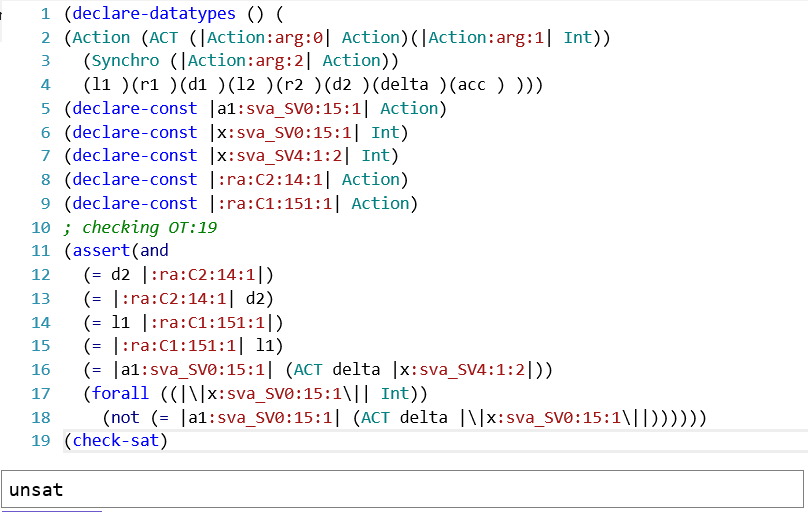
\includegraphics[width=0.8\linewidth]{ActaXFIG/rise4fun1}}
  \caption{Checking one Open Transition in Z3}  \label{schema:smt-lib}
\end{figure}

For simplicity, we have only shown here a use-case with boolean conditions, so we only require the basic SAT capability of the Z3
engine. It should be clear that more involved examples will require
reasoning about predicates of various data types. Z3 provides theories for reasonning
about integers, bitstrings, enumerated types, arrays, etc.
We also need to deal with some universal quantification on free
variables occuring in the guards of synchronisation vectors.
For other data structures  in such models, like records, or
recursive structures, the user will have to develop her own theories.
Decidability of these theories will condition on the completeness of the
satisfiability check, and the decidability of model-checking or
bisimulation checking.




%% \begin{figure}[t]
%%   \centerline{\includegraphics[width=10cm]{XFIG/Interaction}}
%%   \caption{The architecture of the interaction between pNet API and Z3}  \label{schema:interaction}
%% \end{figure}

\paragraph{Production of the SMT-lib code}
  To build the input submitted to Z3 for each OT,
we translate the algebra presentation, the predicates and the
variable assignments into Z3 (Java-API) calls.
% The $presentation$ and the predicates are translated separately. 

\emph{Translation of action algebra presentation.}
In~\cite{AVOCS18}, we  define the translation of an algebra presentation into
SMTlib declarations (\texttt{declare-datatypes} and
\texttt{declare-fun}). We also formalise a condition of well-formedness of pNets to ensure that the generated code is correct
and will not raise runtime errors in the SMT engine. Note that the
\texttt{declare-datatypes} command comprises both the action
constructors from Table~\ref{table:BIPalgebra} and also the constant action
names from our example.
In addition, we will include the axiomatisation of any required functions
and predicates of the presentation data-types.


%% \paragraph{Translating assignments into predicate terms.}
%% State variable assignments that were collected during the open
%% automaton are used when generating the SMTlib asserts (see
%% App.~\ref{appendix:translating-assignments}). \noteSB{I am not an expert of Z3 or SMT-LIB, but the clause '\texttt{(= t (- t 1))}' looks very suspicious to me.}\hl{This appears in
%% line 10 of Figure~\ref{schema:smt-lib}, which encodes possible values of
%% the variable $t$ of the timer.}

%The assignments are also taken into account when checking the
%satisfiability of the open transitions as they represent the value of
%the variables involved in an OT. In order to do that, we employs a
%translation from assignments into term of predicates. The assignments
%required to be translated are only those belong to the variables
%contain in the start states of the open transitions. The assignments
%are represented as equations between the variables and the expressions
%on the right side of assignment. For the assignments of the same
%variable, we do not figure out which state is the precursor of current
%state, we keep all these possible equations instead, and generate the
%disjunction of these equations. The state could always move to the
%target state if there exists one of the values of its variable
%satisfies the guard.
%%\TODO{It won't matter the variable of the next state
%%except that the right hand side expression contain its variables. This
%%is a problem left to be solved in our future work. WHICH PROBLEM ?}
%After that, for the assignments of the different variables, we generate a conjunction of them. This way we obtain a new term of the predicate involving assignments of the variables.

%% State-variable assignments are also treated as a part of the
%% predicates when checking the satisfiability. % Here we need conduct some
%% % translations,
%% For each assignement in a $\Post$ predicate, such as $\{s_0 \leftarrow 1\}$ in section
%% ~\ref{section:op-semantics}, we translate it into an equation
%% $s_0=1$. For several assignments of the same variable in the same state,
%% we generate the disjunction of 
%% these equations. Correspondingly, we generate a conjunction for the
%% assignments from different variables. 


\emph{Translation of open transitions.}
In~\cite{Avocs-RR} we formally define all steps of the translation of each
open transition, including:
%
\begin{itemize}
	\item to collect all variables in the transition, and declare them (using \texttt{declare-const}),
	\item to check the well-formedness and correct typing of expressions,
	\item to translate the predicate into a conjunction of assertions,
	\item to translate the state-variable
	assignments into a disjunctive assertion, if the assignments are present in the source state.
\end{itemize}
%
This translation ensures that no runtime error will occur
in the SMT engine.

Figure~\ref{schema:smt-lib} shows the decomposition of the
predicate into a set of asserts, each encoding an elementary equality,
inequality, or a guard. 
The result (SAT or UNSAT) of the final \texttt{check-sat} command in
the translation is then decoded.

\section{Use-Cases}
\label{section:use-cases}
In this section we present the results of open automata construction
for several examples, starting with three constructions from
Section~\ref{section:running-example} using the Enable operator.
Then we give detailed results for the Failure Controller that was
presented in \cite{AVOCS18}, and show how this sort of BIP architectures
can be composed together.
Finally, we give some figures illustrating the benefits of the smart
algorithm on these examples.

\subsection{Enable operator} 
\label{section:use-case:Enable}

\vspace{-5mm}
\begin{figure}[ht]
\centerline{ 
  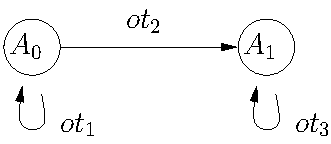
\includegraphics[width=0.25\linewidth]{ActaXFIG/Enable1-aut}
  \hspace{25mm}
  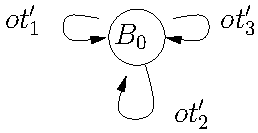
\includegraphics[width=0.20\linewidth]{ActaXFIG/Enable2-aut}}
  \begin{minipage}{5.7cm}
$  \begin{array}{@{}r@{}l@{}}
    ot_1  = &\openrule{\{ \xrightarrow{a1}_P \},\\ [\forall x1. a1\neq\delta(x1)]}
    {A_0 \xrightarrow{a1} A_0}\\
    ot_2  =& \openrule{
                            \{\xrightarrow{\delta(x2)}_P,\,
                            \xrightarrow{acc(x2)}_Q\}  }
    {A_0 \xrightarrow{\underline{\delta(x2)}} A_1}\\
    ot_3  =& \openrule{
                          \{  \xrightarrow{a3}_q \},\\ [\forall x3. a3\neq\delta(x3)] }
    {A_1 \xrightarrow{a3} A_1}
  \end{array}$
  \end{minipage}
  \hspace{2mm}
  \begin{minipage}{6cm}
$  \begin{array}{@{}r@{}l@{}}
    ot'_1  =& \openrule{
    	\{\xrightarrow{b1}_P\}, ~~ [\forall y1. b1\neq\delta(y1) \!\land\! v=0]}
    {B_0 \xrightarrow{b1} B_0}\\
    ot'_2  =& \openrule{
                            \{\xrightarrow{\delta(y2)}_P,\,
                            \xrightarrow{acc(y2)}_Q \}, \\
                                        v=0, \\
                                        \{v\gets 1\}}
    {B_0 \xrightarrow{\underline{\delta(y2)}} B_1}\\
    ot'_3  =& \openrule{
                            \xrightarrow{b2}_q, \\ [\forall y2. b2\neq\delta(y2) \!\land\! v=1] }
    {B_1 \xrightarrow{b2} B_1}
  \end{array}$
  \end{minipage}
  \caption{The two open automata}
  \label{schema:enable-OAs}
\end{figure}

The open automata generated for the two encodings of Enable in
Figure~\ref{schema:enable-pnets} are displayed in
Figure~\ref{schema:enable-OAs}.
Note that although these automata look very similar to the PLTS
controllers from Figure~\ref{schema:enable-pnets}, their nature is very
different: they represent the behavior of the whole system, including
the holes $P$ and $Q$. Their transitions do not rely on a particular
implementation of the controllers, but only encode the 
relations between the actions of the holes.
We have shown in \cite{henrio:Forte2016} how to prove that they are bisimilar.
 
%%\subsection{simple communication protocol} specification and implementation;
%%\TODO{Eric: more results: enable associativity}


\begin{figure}[h]
  \begin{minipage}{2cm}
  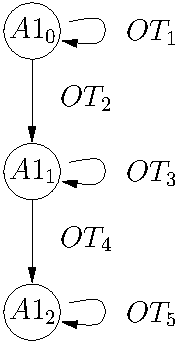
\includegraphics[width=0.9\linewidth]{ActaXFIG/PQR-automaton}
  \end{minipage}
  \hspace{10mm}
  \begin{minipage}{3.5cm}
  \begin{eqnarray*}
    OT_1 & = \openrule{\{\xrightarrow{a1}_P\}\\ a1\neq\delta(x)}
    {\ostate{00} \xrightarrow{a1} \ostate{00}}\\
    OT_2 & = \openrule{
                            \{\xrightarrow{\delta(x1)}_P, ~~
                            \xrightarrow{acc(x1)}_Q\}
                      }
                      {\ostate{00} \xrightarrow{\underline{\delta(x1)}} \ostate{10}}    \\
    OT_3 & = \openrule{
                        \{\xrightarrow{a2}_Q\},\\a2\neq\delta(x)
                        }
    {\ostate{10} \xrightarrow{a2} \ostate{10}}
    \end{eqnarray*}
  \end{minipage}
  \hspace{10mm}
  \begin{minipage}{4cm}
  \begin{eqnarray*}
    OT_4 & = \openrule{
                      \{\xrightarrow{\delta(x2)}_Q, \qquad 
                       \xrightarrow{acc(x2)}_R\} 
                       }
                      {\ostate{10} \xrightarrow{\underline{\delta(x2)}} \ostate{11}}    \\
    OT_5 & = \openrule{\{\xrightarrow{a3}_R\}
    	}
    {\ostate{11} \xrightarrow{a3} \ostate{11}}
    \end{eqnarray*}
  \end{minipage}
  \caption{Open Automaton for the term ``$P>>(Q>>R)$''}
  \label{schema:enable3bis}
\end{figure}

Now let us revisit the Enable composition from
Figure~\ref{schema:enable-composed}. Its open automaton is shown in
Figure~\ref{schema:enable3bis}. Building the symmetric system ``$(P>>Q)>>R$'' in a similar
way will allow us to prove that they are bisimilar (the Enable
operator is associative), as we have shown in \cite{HMZ:RR-2016}.
This approach allows us to study the equational properties of
many operators in classical process algebras or parallel languages, even
when their semantics depends on data properties.

\subsection{BIP Failure Monitor Architecture}
\label{section:FailureTimer}


In this section, we present the Failure Monitor architecture from the
CubETH nanosatellite on-board software
case-study~\cite{CubETH-case-study} realised using BIP.
The architecture-based design process in BIP takes as input a set of
components providing basic functionality of the system and a set of
temporal properties that must be enforced in the final system.  For
each property, a corresponding architecture is identified
and applied to the model, thereby potentially introducing additional
coordinator components and modifying the connectors that define
synchronisation patterns among ports of components.

\begin{figure}[t]
  \centering
  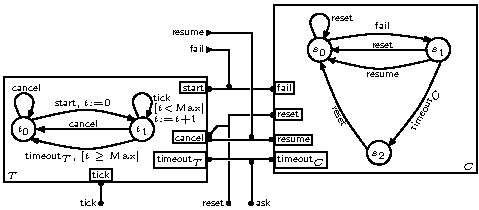
\includegraphics[width=\columnwidth]{ActaXFIG/BIPspec-ArchFailureTimer-v2-2}
  \caption{The BIP specification of the Failure Monitor architecture}
  \label{schema:ArchFailure:BIP}
\end{figure}

Figure~\ref{schema:ArchFailure:BIP} shows a refined version of the
Failure Monitor architecture used in~\cite{CubETH-case-study}.
%
The architecture consists of 2 \emph{coordinator components}
($\NameCtrl$ and $\NameTimer$, for \emph{Control} and \emph{Timer},
respectively), 5 \emph{dangling ports} ($\PortFail$, $\PortResume$,
$\PortTick$, $\PortReset$ and $\PortAsk$) and 5 connectors.
%
%% Contrary to standard BIP models, architectures comprise one or several
%% \emph{operand} components, whereof only the set of \emph{ports} is
%% given.  Here, the operand component is $\NameOprnd$ and its interface
%% consists of the ports $\PortResume$ and $\PortFail$.
%% The two \emph{coordinator} components\mdash $\NameCtrl$ and
%% $\NameTimer$\mdash are standard
The  \emph{behaviour} of BIP components %% insofar as they also
%% have their 
is specified by finite automata extended with
local data variables.  Transitions of these automata are labelled with
the ports of the corresponding components, Boolean guards and update
functions on local variables.  %% For instance, the loop transition
%% $t_1 \goesto{\PortTick, [t < Max], t:=t+1} t_1$
%% in the $\NameTimer$ component is labelled by the port $\PortTick$. It
%% can be fired only when the current value of the local variable $t$ is
%% lower than $Max$.  Upon firing, this transition increments the value
%% of $t$ by $1$.  When omitted, the default guard (\resp update
%% function) is the constant predicate $\true$ (\resp the $\mathit{skip}$
%% operator).  The constant $\mathrm{Max}$ above, is a parameter of the
%% architecture.
Although this is not visible in the figure, below we will assume that
the dangling ports $\PortFail$ and $\PortResume$ belong to the operand
component, whereas the dangling ports $\PortTick$, $\PortAsk$ and
$\PortReset$ represent actions of the environment.  

%% Connectors are hierarchical, tree-like structures with component ports
%% at the leaves.  They define sets of \emph{interactions}, 
Based on the
attributes of the connected ports, which may be
either \emph{triggers} (triangles in Figure~\ref{schema:ArchFailure:BIP})
or \emph{synchrons} (bullets in Figure~\ref{schema:ArchFailure:BIP}),
%
connectors specify the syncrhonisations (also called
\emph{interactions}) between the transitions of the individual
components.  Intuitively, triggers can initiate interactions, whereas
synchrons can only join.  If a connector does not have triggers, all
the involved ports must synchronise~\cite{BliSif08-acp-tc}.
%% %
%% If all the sub-connectors of a connector are synchrons, then an
%% interaction may be executed by the connector only if each subconnector
%% can contribute.
%% %
%% If at least one of the sub-connectors is a trigger, then any
%% interaction consisting of contributions of any set of sub-connectors,
%% \emph{involving at least one of the triggers}, can be executed.
%
For instance, the two ports $\NameTimer.\PortStart$ and
$\NameCtrl.\PortFail$ are always synchronised, since they belong to
the same binary sub-connector, where they are both synchrons.  In
particular, this means that whenever the transition 
$\cstate{0} \goesto{\PortFail} \cstate{1}$ is fired, so is the transition
$\tstate{0} \goesto{\PortStart, t:=0} \tstate{1}$,
initialising the timer.  The binary connector $\NameTimer.\PortStart
\bullet\!\!\!-\!\!\!-\!\!\!\bullet \NameCtrl.\PortFail$ is a
sub-connector of a hierarchical connector, where the dangling port
$\NameOprnd.\PortFail$ is a trigger.  Thus, the above interaction can
only happen together with $\NameOprnd.\PortFail$, forming a
ternary interaction.  On the contrary, being a trigger, the port
$\NameOprnd.\PortFail$ can fire alone, forming a singleton
interaction.  The composition semantics of BIP systems consists in
firing exactly one interaction, enabled through at least one of the
top-level connectors, at each execution round.

%% Finally, \emph{priorities}\mdash defined by a strict partial order on
%% the set of possible interactions\mdash narrow the choice among the
%% enabled interactions at any given round.  The default priority is the
%% so-called \emph{maximal progress}, whereby among any two interactions
%% $a \subset b$ (as sets of ports), $b$ has higher priority than $a$.
%% For example, the port $\NameOprnd.\PortFail$ will never fire alone in
%% a global state, where both $\NameTimer.\PortStart$ and
%% $\NameCtrl.\PortFail$ are enabled.

%
%% Adding priorities $\NameOprnd.\PortFinish < \NameCtrl.\PortReset$ and
%% $\NameOprnd.\PortFinish < \NameOprnd.\PortResume$, ensures that, after
%% a failure, the operation performed by $\NameOprnd$ cannot finish
%% unless it is explicitly resumed or the system is reset.

Notice that the model in Figure~\ref{schema:ArchFailure:BIP} allows
$\PortReset$ to happen in any state.  However, it is implied that,
when the coordinator $\NameCtrl$ is in state $\cstate{2}$, this
$\PortReset$ is ``asked for'' by the architecture (it follows the
firing of $\PortAsk$), whereas in other states the corresponding
transition reflects an ``external'' reset.  Although this can be
formalised in the model using data variables, we have chosen not to do
so for the sake of simplicity.

Intuitively, application of the Failure Monitor architecture ensures
that, whenever a failure is registered in the operand component, the
system will be reset, unless a resumption is registered within
$\mathrm{Max}$ time units.  Formally, this statement is decomposed
into several properties, among which 
%
1)~the safety property \emph{``A reset is never asked for unless a failure occurs''} specified using CTL as
%
\begin{equation}
  \label{eq:FM:safety}
  %% \AG
  %% \bigl(\PortFail \rightarrow
  %% \EX \EU[]{\lnot \PortFail}{\PortReset}\bigr)
  \AW[]{\lnot \PortAsk}{\PortFail}
\end{equation}
%
and 2)~the liveness property \emph{``in the absence of an external
  reset, a reset can always be asked for after a non-transient
  failure''}:
%
\begin{equation}
  \label{eq:FM:liveness}
  %% \mathtt{AG}(\PortAsk \rightarrow \mathtt{AF}\ \PortReset).
  \AG \bigl(
  \PortFail \rightarrow \EU[]{(\lnot \PortReset \land \lnot \PortResume)}{\PortAsk}
  \bigr)
\end{equation}
%
Additional properties are provided in~\cite{Avocs-RR}.


%% \TODO{it would be good to express here maybe 2 properties of the
%%   architecture, maybe one taken from the original study, and another
%%   one involving the timer data (number of ticks ?)}

\begin{figure}[t]
  \centering
  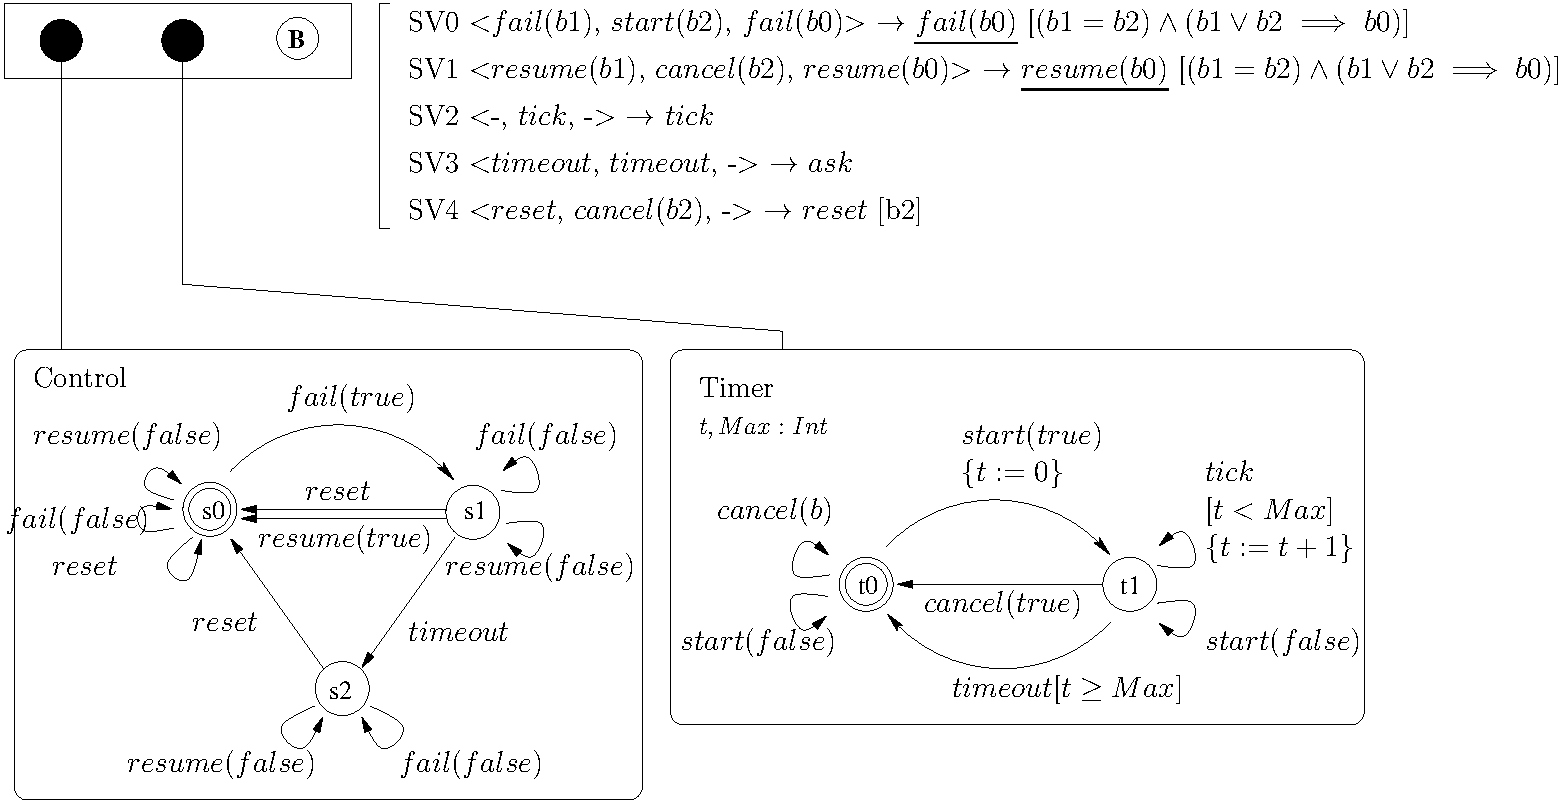
\includegraphics[width=0.9\columnwidth]{ActaXFIG/FailureTimerPNET-v2-2}
  \caption{pNet encoding of the Failure Monitor architecture}
  \label{schema:ArchFailure:pNet}
\end{figure}

Figure~\ref{schema:ArchFailure:pNet} shows a pNet encoding of the
above Failure Monitor architecture.  This encoding is structural: each
coordinator component is encoded as a PLTS; dangling ports belonging
to the operand component are encoded as actions of the hole; 
%%  and the operand component as a hole;
connectors of the BIP model are encoded as synchronisation vectors,
with ports
  representing the actions of the environment used as global actions.
Each connector that does not involve triggers is trivially encoded by
a synchronisation vector comprising the same ports ($SV2$, $SV3$ and
$SV4$).  In order to encode the semantics of the connectors involving
triggers, we use (in $SV0$ and $SV1$) the classical approach where
non-participation of a port in an interaction is simulated by an
additional loop transition~\cite{milner83-calculi}.  To this end, we
consider an action algebra involving additional Boolean variables: the
effective transitions carry the value $\true$ (\eg $\cstate{0}
\goesto{\PortFail(\true)} \cstate{1}$), whereas the added loops carry
the value $\false$ (\eg $\cstate{2} \goesto{\PortFail(\false)}
\cstate{2}$).  In the synchronisation vectors, we use these variables
to encode the connector structure as a Boolean predicate.  For
example, $SV0$ encodes the connector discussed above: the predicate
$(b1=b2) \land (b1\lor b2 \Rightarrow b0)$ means that the ``true''
transitions $\NameCtrl.\PortFail$ and $\NameTimer.\PortStart$ can only
fire together ($b1 = b2$) and whenever one of them fires,
$\NameOprnd.\PortFail$ must fire also ($b1 \lor b2 \Rightarrow b0$).
This encoding can be systematically obtained for any hierarchical BIP
connector~\cite{BliSif10-causal-fmsd}.
%
%% \noteEM{Decide later if this is still useful}Although, for the sake of
%% brevity, we omit priorities from the encoding, this can be easily
%% achieved, by introducing another set of additional Boolean variables
%% for relevant ports~\cite{BarBliu15-offer-scico}.



\paragraph{Computed open automaton.}

For this example, the tool (using Algorithm~\ref{alg1}) builds 408 open transitions, whereof 396
are detected unsatisfiable by Z3.  The resulting open automaton, with
3 reachable global states (out of the possible 6) and 12 open
transitions, is shown in Figure~\ref{schema:resultOA1}.
%% \noteSB{Eric, in the state 20, $b0$ should always be $false$: $\PortFail(true)$ is not possible in Control, and the safety property (\ref{eq:FM:safety}) does not hold otherwise.}

\begin{figure}[t]
  \centerline{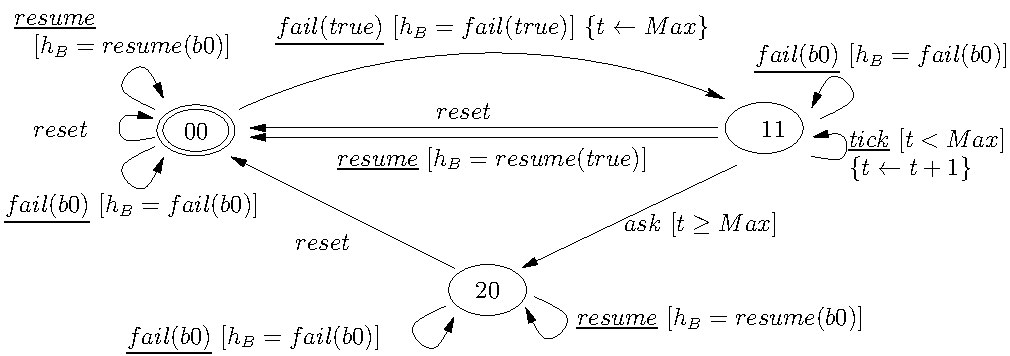
\includegraphics[width=12cm]{ActaXFIG/FailureTimerOA-v2-2}}
  \caption{Open Automaton for the Failure Monitor architecture}
  \label{schema:resultOA1}
\end{figure}

%% To improve the readability of this figure, we used the following conventions:
%% we omit the transitions of the two PLTS, and the set of ``working''
%% holes; and we directly write the resulting action as first element of
%% each OT, rather than including it as an equality inside the
%% predicate.
%
%Notice, however that the loop transitions
%$\underline{\mathit{resume}}$ in states $\ostate{s0,t0}$ and
%$\ostate{s2,t0}$, corresponding, respectively, to open transitions
%$ot_2$ and $ot_9$ in Figure~\ref{schema:ots} of
%App.~\ref{appendix:fullOutput}, involve $\OTvar{resume(false)}$ from
%the two PLTS, \ie only the hole, corresponding to the operand
%component of the Failure Monitor architecture, executes $\PortResume$.

The satisfaction of the safety property (\ref{eq:FM:safety}) could be
established by applying symbolic model checking techniques.  However,
in this example, it is obvious by inspection of the open automaton.
The satisfaction of the liveness property relies on the observation
that in the state $\ostate{s2,t0}$ only the reset transition involves
$\NameCtrl$.  Therefore, under resonable scheduling assumptions,
$\PortReset$ will always be fired.

\subsection{Composing Two Failure Monitor BIP Architectures}
\label{section:use-case:Double}

%% In the design of the nanosatellite software \cite{CubETH-case-study}, the Failure Monitor architecture was used to control several processes
%% communicating through a common bus. Timeout signals (``$ask$''), resets,
%% and the passing of time ($tick$) were synchronised in the global
%% system.
In this section, we use a combination of two Failure Monitor
architectures shown in Figure~\ref{schema:ArchFailure:BIP:Double}
%% to demonstrate how the encoding works, and
as a slightly larger example to show how the approach scales up.  In
this example, each of the two instances of the architecture is applied
to a corresponding operand component.  Hence, the dangling ports
$\PortFail$ and $\PortReset$ are duplicated accordingly.  On the
contrary, the environment actions $\PortTick$, $\PortAsk$ and
$\PortReset$ are shared.  For a detailed presentation of the
architecture composition, we refer the reader to
\cite{AttieBBJS16-architectures-faoc}.

\begin{figure}[ht]
  \centering
  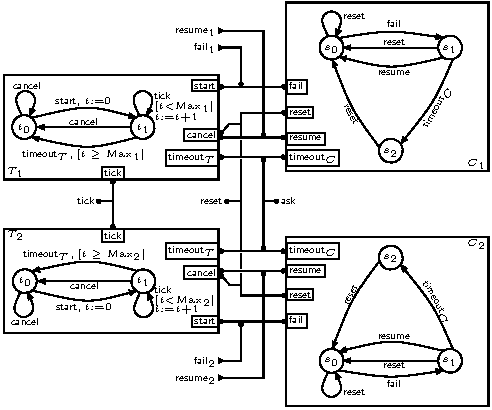
\includegraphics[width=0.9\columnwidth]{ActaXFIG/BIPspec-DoubleArchFailureTimer-v2-2}
  \caption{The BIP specification of two composed Failure Monitor architectures}
  \label{schema:ArchFailure:BIP:Double}
\end{figure}

\begin{figure}[ht]
  \centering
  %% 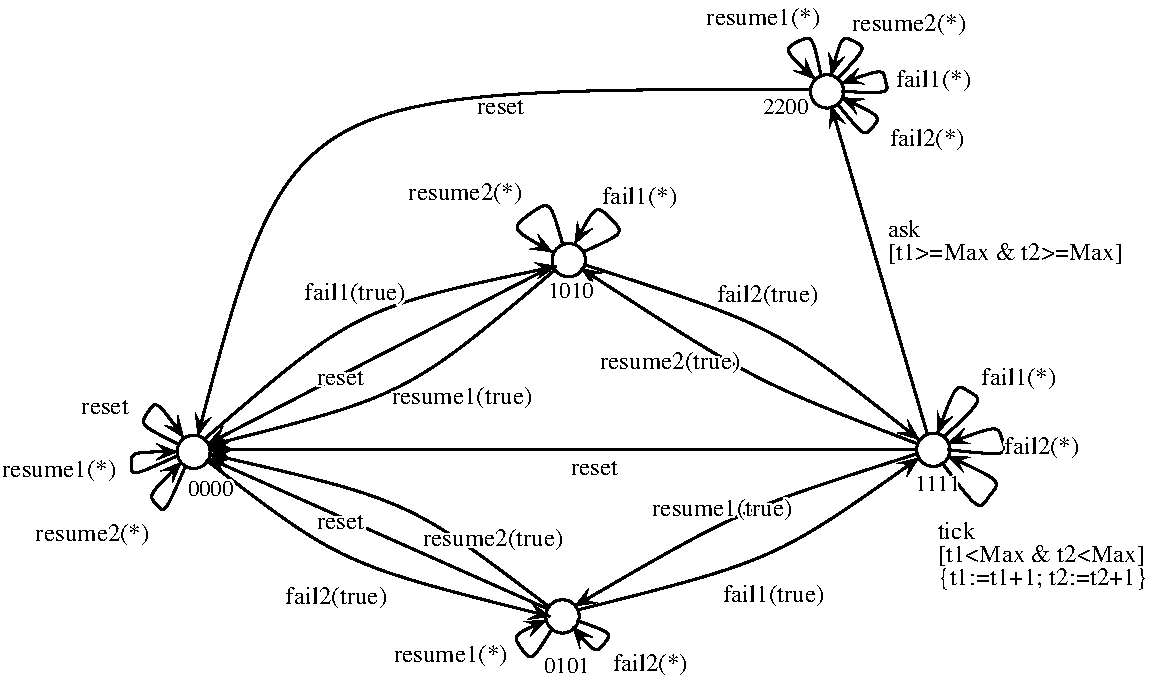
\includegraphics[width=0.9\columnwidth]{ActaXFIG/Double-OA}
  \resizebox{\columnwidth}{!}{
  \begin{tikzlts}
    \node[state] (0000) {0000};
    \node[state, above right= 10mm and 30mm of 0000] (1010) {1010};
    \node[state, below right= 10mm and 30mm of 0000] (0101) {0101};
    \node[state, below right= 10mm and 30mm of 1010] (1111) {1111};
    \node[state, above right= 15mm and 20mm of 1010] (2200) {2200};

    \path[draw,->]
    (0000.135)
    .. controls +(-7mm,3mm) and +(-3mm,7mm) ..
    node {reset}
    (0000.120)
    ;

    \path
    (0000)
    edge[loop left] node[left] {resume1(*)} (0000)
    edge[bend left] node[above] {fail1(true)} (1010)
    edge[bend right] node[below] {fail2(true)} (0101)
    ;

    \path[draw,->]
    (0000.-120)
    .. controls +(-3mm,-7mm) and +(-7mm,-3mm) ..
    node[below left] {resume2(*)}
    (0000.-135)
    ;

    \path[draw,->]
    (1111.60)
    .. controls +(3mm,7mm) and +(7mm,3mm) ..
    node[above right] {fail1(*)}
    (1111.45)
    ;

    \path
    (1111)
    edge node {reset} (0000)
    edge[loop right] node[right] {fail2(*)} (1111)
    edge[out=170,in=-20] node[left] {resume2(true)} (1010)
    edge[out=-170,in=20] node[left] {resume1(true)} (0101)
    ;

    \path[draw,->]
    (1111.-45)
    .. controls +(7mm,-3mm) and +(3mm,-7mm) ..
    node[below right] {\begin{tabular}{@{}l@{}}
        tick\\
        {}[t1 < Max1 \& t2 < Max2]\\
        \{t1:=t1+1; t2:=t2+1\}
    \end{tabular}}
    (1111.-60)
    ;
    
    \path[draw,->]
    (1111) edge
    node[above right] {\begin{tabular}{@{}l@{}}
        ask\\
        {}[t1 $\geq$ Max1 \& t2 $\geq$ Max2]
    \end{tabular}}
    (2200)
    ;

    \path
    (1010)
    edge[out=-170,in=30] node[above] {reset} (0000)
    edge[out=-150,in=20] node[below] {resume1(true)} (0000)
    edge[bend left] node[above] {fail2(true)} (1111)
    ;

    \path[draw,->]
    (1010.45)
    .. controls +(7mm,3mm) and +(3mm,7mm) ..
    node[above right] {fail1(*)}
    (1010.80)
    ;
    
    \path[draw,->]
    (1010.100)
    .. controls +(-3mm,7mm) and +(-7mm,3mm) ..
    node[above left] {resume2(*)}
    (1010.135)
    ;

    \path
    (0101)
    edge[out=170,in=-30] node[below] {reset} (0000)
    edge[out=150,in=-20] node[above] {resume2(true)} (0000)
    edge[bend right] node[below right] {fail1(true)} (1111)
    ;

    \path[draw,->]
    (0101.-45)
    .. controls +(7mm,-3mm) and +(3mm,-7mm) ..
    node[below right] {fail2(*)}
    (0101.-80)
    ;
    
    \path[draw,->]
    (0101.-100)
    .. controls +(-3mm,-7mm) and +(-7mm,-3mm) ..
    node[below left] {resume1(*)}
    (0101.-135)
    ;

    \path[draw,->]
    (2200.west)
    .. controls +(left:5cm) ..
    node[above left] {reset}
    (0000.80)
    ;

    \path[draw,->]
    (2200.0)
    .. controls +(7mm,0) and +(3mm,-7mm) ..
    node[right] {fail2(*)}
    (2200.-20)
    ;
    
    \path[draw,->]
    (2200.40)
    .. controls +(3mm,7mm) and +(7mm,3mm) ..
    node[above right] {fail1(*)}
    (2200.20)
    ;
    
    \path[draw,->]
    (2200.100)
    .. controls +(-3mm,7mm) and +(3mm,7mm) ..
    node[above] {resume2(*)}
    (2200.80)
    ;
    
    \path[draw,->]
    (2200.160)
    .. controls +(-7mm,3mm) and +(-3mm,7mm) ..
    node[left] {resume1(*)}
    (2200.150)
    ;
  \end{tikzlts}}
  \caption{The resulting automaton}
  \label{schema:ArchFailure:Double:OA}
\end{figure}

%% In Figure~\ref{schema:ArchFailure:BIP:Double} we show the combination
%% of two Failure Monitor architectures, with their respective controlled
%% processes.
In Figure~\ref{schema:ArchFailure:Double:OA} we show the open
automaton computed for the combined architecture of
Figure~\ref{schema:ArchFailure:BIP:Double}.
%
Comparing the guards of the transitions $\PortTick$ and $\PortAsk$
leaving state $1111$, we see that $\PortAsk$ can never be taken,
unless $\mathrm{Max1} = \mathrm{Max2}$.  This illustrates the
\emph{interference} phenomenon discussed in
\cite{AttieBBJS16-architectures-faoc}, showing that the liveness
property (\ref{eq:FM:liveness}) is not preserved when two copies of
the Failure Monitor architecture are composed together.\footnote{%
%
  One of the main results of \cite{AttieBBJS16-architectures-faoc}
  states that in a system obtained by an application of several
  architectures, liveness properties are preserved if these
  architectures are \emph{pair-wise non-interfering}.  However, no
  results were provided to check whether two architectures are
  interfering or not.
%
} In this example, the interference is caused by the strong
synchronisation of the $\PortTick$ ports of the two architectures.  It
can be avoided by replacing the \mbox{$\PortTick
  \bullet\!\!\!-\!\!\!-\!\!\!\bullet \NameTimer.\PortTick$} connector
in Figure~\ref{schema:ArchFailure:BIP} by \mbox{$\PortTick
  \blacktriangleright\!\!\!-\!\!\!-\!\!\!\bullet
  \NameTimer.\PortTick$} and applying the so-called \emph{maximal
  progress} whereby, whenever possible, the interaction $\{\PortTick,
\NameTimer.\PortTick\}$ is preferred to the firing of $\PortTick$
alone.  However, this fix goes beyond the scope of the current paper.

%% It indicates that the two
%% timers are forced to be synchronous: each can only tick after the
%% other has also started, and then they will tick, reset, and timeout,
%% synchronously.
%% %
%% \hl{This is a very strong assumption, and we are working on a more
%% flexible specification (at BIP level) to release this hypothesis while
%% keeping the safety properties of the composition.}

%% \noteInSB{The idea was that, by analysing the combination, we observe
%%   that the architecture does not compose well with itself, generating
%%   a deadlock (or an implicit deadlock, where only $false$ transitions
%%   canb be fired.  Based on this observation, we were to improve it
%%   accodingly.  The problem is that I do not see any deadlocks in
%%   Figure~\ref{schema:ArchFailure:Double:OA}.  I presume that some of
%%   the asterisks should be only $false$ or something of a kind.}




\subsection{Benefits from the Smart Algorithm}

In each cell of the following table, we display the number of OTs whose predicates were found SAT/UNSAT by the SMT engine, and the overall time spent for the execution of the whole algorithm.

All tests are run on HP EliteBook 840 laptop under Windows 10 x64, with an Intel quad-Core i7-6600U
processor, and 32Gb of RAM. The software platform is VerCors\footnote{Available at \url{https://team.inria.fr/scale/software/vercors/}.}, running on top of
Eclipse Equinox, with Java 1.8.


	\begin{tabular}{p{4cm}p{3cm}p{3cm}}
		\hline\specialrule{0em}{1pt}{1pt}
		Use-case & Brute force & Smart algorithm
                \\\specialrule{0em}{1pt}{1pt}
		\hline\specialrule{0em}{3pt}{3pt}
		Enable operator   			&
                3/6 OTs           &
                3/6 OTs
                \\\specialrule{0em}{1pt}{1pt} 
                State-based 		&
                125 ms 				&
                110 ms  
		\\\hline\specialrule{0em}{3pt}{3pt}
		Enable operator   			&
                3/6 OTs           &
                3/6 OTs
                \\\specialrule{0em}{1pt}{1pt} 
                Data-based 		&
                141 ms 				&
                205 ms  
		\\\hline\specialrule{0em}{3pt}{3pt}
		Enable Composition   			&
                5/55 OTs           &
                5/42 OTs
                \\\specialrule{0em}{1pt}{1pt} 
              %  ``$P<<(Q<<R)$'' 
                State-based		&
                359 ms 				&
                297 ms  
		\\\hline\specialrule{0em}{1pt}{1pt}
		FailureTimer    			&
                12/396 OTs           &
                12/192 OTs
                \\\specialrule{0em}{1pt}{1pt} 
  		&
                1220 ms 				&
                687 ms  
		\\\hline\specialrule{0em}{1pt}{1pt}
		FailureTimer X 2    			&
                25/8964 OTs           &
                25/1255 OTs
                \\\specialrule{0em}{1pt}{1pt} 
		&
                18088 ms 				&
                3266 ms  
		\\\hline
	\end{tabular}

        \medskip
        In the basic cases ($EnableState$, $EnableData$) there is no
        benefit, and even an overhead in the case of $EnableData$,
        because of the extra step of checking SAT at the end of the
        algorithm.
But as soon as there are more OTs in the system and not all
states are reachable, these tests show a significant benefit of the ``smart'' strategy, in
the considered use-cases, with 50\% of time saving for the $FailureTimer$,
over to 80\% for the composition, depending
        on the nature of the examples, but increasing significantly
        with their complexity.

\section{Conclusion and Discussion}
\label{section:conclusion}

The formal definitions and properties of the open pNets model were
given in \cite{henrio:Forte2016}. In the current work we describe an implementation of
the model and its semantics construction, including its interaction
with the Z3 SMT engine.
The implementation has two parts: the first is an algorithm
that builds all possible combinations of synchronisations through the
pNet hierarchical structure. The result is a so-called
open automaton, whose transitions contain predicates relating
the actions of the pNet holes and controllers. Some of the open
transitions obtained at this step  may
contain predicates which do not represent any possible concrete
instantiations. 
In the second part of the tool we use the SMT solver Z3 to check the
satisfiability of the predicate in each open transition. 
To this end, we encode into Z3 the representations of the action algebra and
the predicates before submitting them to the
Z3 solver. 
%
%\hl{%
%
We have used a running example based on two possible
encodings of the Enable operator of LOTOS. The automata computed with
the algorithm can be used to prove equational properties of the
operator.

Then we define a ``smart'' version of the algorithm that explores, as
much as possible, only the reachable part of the open automaton. The
handling of assignments makes the reachable computation more
challenging. We show that the result is equivalent to the original
algorithm. 

We validate the approach on two larger examples, 
based on a BIP architecture taken from an earlier nanosatellite case
study~\cite{CubETH-case-study}. We also show how such architectures
can be composed, and how our approach scales.
This example shows that
open-automata-based semantics can be instrumental in verifying the
properties enforced by the architectures through an encoding into open
pNets.
We also compare the practical performances of the two algorithms and
show the benefit gained using the smart approach.

Naturally, our next goals after the generation of the open automata
will be to model-check logical properties, and to check equivalences
of pNets. While model-checking open automata seems easy to define,
equivalence checking is more challenging. 
In~\cite{henrio:Forte2016}, we
have already found the FH-bisimulation 
to be a suitable definition. But weak equivalences, or refinements, will
definitely be useful when comparing different pNets with
different structures. For both model-checking and bisimulation, SMT methods
will be the basis for comparing open transitions. 


%% \emph{Scaling up.} One important motivation of this work is to
%% attack the complexity of verification of realistic systems by a
%% compositional and parametric approach. Still one may wonder if the price
%% for analysing our symbolic transitions will not make the approach too expensive
%% in terms of computing time. We tried a
%% slightly bigger example, assembling two Failure
%% controllers. In~\cite{Avocs-RR}, we show that Z3 can check the 
%% satisfiablility of  90K open transitions in a couple of minutes.


\bibliographystyle{spmpsci}
\bibliography{biblio}


\appendix

\section{Semantic Rules of pNets }
\label{appendix:semRules}

To facilitate the understanding of the two algorithms, we briefly recall the semantic rules of pNets, more details can be found in \cite{henrio:Forte2016}.

We build the semantics of an open pNet as an open automaton where
LTSs are the PLTSs at 
the pNet leaves, and the states of the automaton are structured. 
To build an open transition we first
 projects the global state into states of the leaves, then apply
PLTS transitions on these states, and compose them with actions of
holes using synchronisation vectors. 

The semantics   regularly instantiates \emph{fresh} variables, and uses a
\emph{clone} operator that clones a term replacing each variable with a
fresh one.
The variables in each synchronisation vector are considered local:
for a given pNet expression, we must have fresh local variables for
each occurrence of a vector. %(= each time we instantiate rule Tr2). 
Similarly, the state variables of each copy of a
given PLTS in the system must be distinct, and those created for each
application of Tr2 have to be fresh and all distinct. 


\begin{definition}[Operational semantics of open pNets]
  \label{def:operationalSemantics}
  The semantics of a pNet $p$ is an open automaton $A = \langle Leaves(p),J,\mathcal{S}, s_0,
  \mathcal{T}\rangle $ where:
  \begin{itemize}
    \item $J$ is the indices of the holes: $Holes(p)= H_j^{j\in J}$.
    %  \item $\overline{L}^L = Leaves(p), \overline{H}^J = Holes(p)$
    \item $\overline{\mathcal{S}} = States(p)$ and $s_0 = InitState(p)$
    \item $\mathcal{T}$ is the smallest set of open transitions
    satisfying the rules below:
  \end{itemize}
  
  The first rule ({\bf Tr1}) for a PLTS $p$  checks that the guard 
  is verified and transforms assignments into post-conditions:
  
  \begin{description}
    \item[{\bf Tr1:}]
    $\inferrule
    { s \xrightarrow{\langle \alpha,~e_b,~(x_j\!:= {e}_j)^{j\in
          J}\rangle} s'\in \to  \\
      {\tt fresh}(v) \\
      Pred = ~e_b \land (v = \alpha)
    }
    { p = \langle  S,s_0, \to \rangle
      \models
      \inferrule*[myfraction=\reddottedrule]
      {\{s \xrightarrow{\alpha}_p s'\} ,\emptyset ,
      Pred,\left\{x_j\gets e_j\right\}^{j\in J}}
      {\ostate{s} \xrightarrow{v} \ostate{s'}}
    }
    $
  \end{description}
  
  The second rule ({\bf Tr2}) deals with pNet nodes: for each possible
  synchronisation vector applicable to the rule subject, the premisses
  include one {\em open transition} for each sub-pNet involved, one possible
  {\em action} for each hole involved, and the predicate relating these
  with the resulting action of the vector.
  A key to understand this rule is that the open transitions are
  expressed in terms of the leaves and holes of the pNet structure,
  i.e. a flatten view of the pNet. For example, in the rule, $L$ is the index set of the leaves of the open pNet, $L_k$ is the index set of the leaves of one subnet, thus all $L_k$
  are disjoint subsets of $L$.
  
  \begin{description}
    \item[{\bf Tr2:}]
  \end{description}
  
  \noindent
    $\inferrule
    {k\!\in\! K \\ SV\!\!= \!clone(SV_k) \!=\! \alpha_m^{m \in I_k\uplus J_k} \!\to\! 
    \alpha'_k, G_k \\
      Leaves(p) \!=\! \pLTS_l^{l\in L} \\     
      \forall m\in I_k.
      \pNet_m \models
      \inferrule*[myfraction=\reddottedrule]
      {\{s_{i}\xrightarrow{a_{i}}_i s_{i}'\}^{i\in I_m^\prime},
      \{\xrightarrow{b_{j}}_j\}^{j\in J'_m}, \Pred_m, \Post_m}
      {\ostate{s_{i}^{i \in L_m}} \xrightarrow {v_m}
        \ostate{s_{i}^{\prime\ i \in L_m}}}
      %\land
      %Leaves(\pNet_m) = \overline{PLTS}^{L_k})
      \\
      I' = \biguplus_{m\in I_k}\!\! I_m'
      \\ J' = \biguplus_{m\in I_k}\!\! J'_m \uplus J_k  \\
      \Pred = \bigwedge_{m\in I_k}\!\! \Pred_m \land
      \MkPred(SV,v_m^{m\in I_k},b_j^{j\in J_k},v)\\
      \forall j\!\!\in\!\! J_k. {\tt 
        fresh}(b_j) \\ {\tt fresh}(v) \\ 
      \forall i\in
      L\backslash I'.\,s'_i=s_i 
    }
    {p = \langle \pNet_i^{i\in I}, S_j^{j\in J}, \symb{SV}_k^{k\in K}\rangle
      \models
      {\inferrule*[myfraction=\reddottedrule]
        {\{s_i\xrightarrow{a_i}_i s_i^{\prime}\}^{i\in I^\prime},
        \{\xrightarrow{b_j}_j\}^{j\in J^\prime}, \Pred, \uplus_{m\in I_k} 
        \Post_m}
        {\ostate{s_i^{i\in L}} \xrightarrow {v}
          \ostate{s_i^{\prime i\in L}}}
      }
    }
    $

  \medskip  
\end{definition}

In rule TR2, the generated predicate is composed of the conjunction of
the predicates of the subnets' OTs, with the additional part encoding
the application of the chosen synchronisation vector.
In \cite{henrio:Forte2016} this last part is defined as:
\[\MkPred(SV_k, a_i^{i\in I}, b_j^{j\in J}, v)\Leftrightarrow
\begin{array}{l}
\exists {(a'_i)}^{i\in I},
{(b'_j)}^{j\in J},v'.\, SV_k={(a'_i)}^{i\in I}, {(b'_j)}^{j\in J}\rightarrow v'
\\~~\land
\forall i\in I.\, a_i=a'_i\land \forall j \in J.\, b_j=b'_j \land v=v'
\end{array}\]

%% This definition is not constructive, but the existentialy quantified
%% variable sets here correspond the subsets of subnets and holes that
%% are effectively involved in vector $SV_k$.
%% Within our algorithm, these subsets have been computed by $Combining$ and
%% passed as arguments to the $Matching$ method, so
%% we can construct this predicate fragment as:

%% \[\Pred(SV, \overline{\pNet},\overline{S}, v) = 
%% \begin{array}{l}
%% \forall {(a'_i)}^{i\in I},
%% {(b'_j)}^{j\in J},v'.
%% \\
%% v_m=a'_i\land \, b_j=b'_j \land v=v' \land G_k
%% \end{array}\]
%% \TODO{Eric: to be checked}

Within Algorithm~\ref{alg1}, these subsets have been computed by the
$Combining$ method and passed as arguments to the $Matching$ method
(cf. Section~\ref{section:implementation}) 

To have some practical interest, it is important to know when Algorithm~\ref{alg1} terminates. The following theorem shows that if an open pNet
has finite synchronisation sets, finitely many leaves and
holes, and each PLTS at its leaves has a finite number of states and
(symbolic) transitions, then Algorithm~\ref{alg1} terminates and the operational semantics of the open pNet is a finite automaton. 

\medskip
\begin{theorem}[Finiteness]\cite{henrio:Forte2016}
%\noindent\textbf{Theorem 1} 
	Let $pnet=\langle \overline{\pNet},\overline{S}, \symb{SV}_k^{k\in K}\rangle$ be an open pNet  with leaves $l_i^{i\in I}$ and holes $h_j^{j\in
		J}$, where the sets $I$ and $J$ are finite. Suppose the synchronisation vectors of all pNets 
	included in  $pnet$   are finite, and 
	% $\forall i \in L.\, finite{(states(l_i))} \text{ and } l_i$ 
	$l_i $ has a finite number of state variables for each $i\in I$. Then the semantics of $pnet$ is an open automaton 
	%$\mathcal{T}$ 
	with finitely many states and transitions.
\end{theorem}
\begin{proof}
  The possible set of states of the open automaton is the cartesian
  product of the states of the pNet $PLTS_i^{i\in I}$, which is finite by
  hypothesis. So the top-level residual loop of Algorithm 1 terminates provided each 
  iteration terminates. The enumeration of open-transitions in line 5 of Algorithm~\ref{alg1} is bounded by the
  number of applications of rule Tr2 on the structure of the
  pNet tree. Since a finite number of synchronisation vectors are applied
  at each node, the number of global open transitions is finite. Similarily, if the number
  of transitions of each PLTS is finite, rule Tr1 is 
  applied a finite number of times. Therefore, each internal loop of Algorithm~1 terminates, and we obtain finitely many deduction trees and
  open transitions.
  \hfill \qed
  \end{proof}

\end{document}

%\newpage
\appendix
\section{Changes from pre-proceedings version}
All minor requests from reviewers (typo, grammar) were already corrected in the preproceedings version.

Request from Reviewer 3, that we had not done in the preproceedings, for matter of space, have now been shortly answered.
More precisely,
\begin{itemize}
\item{} in section \ref{section:op-semantics}, we have added a precise statement of our finiteness theorem, that answers the question about termination of the algorithm.
\item{-} in section \ref{section:pruning} we have added more explanations about the way that various data types theories will be handled by the SMT engine
\end{itemize}


The following appendices are included for the convenience of reviewers.
Our intention is to publish as a research report, before final publication, an
extended version containing all technical details, proofs, and more examples.

The appendices are organized in the following way:

\begin{enumerate}
\item[A] pNet semantic rules
\item[B] Variable management
  \subitem B.1 fresh variables
  \subitem B.2 managment of state variables
\item[C] Algebra presentations
\item[D] Well-formness and typing of expressions
\item[E] Translation to SMTlib input language
\item[F] Full output for the FailureTimer open automaton
\item[G] Scaling up
  
\end{enumerate}


\section{pNet semantic rules}
\label{appendix:semRules}

\paragraph{Note:} For convenience, we have included here the semantic rules for pNets,
that were already published in \cite{henrio:Forte2016}.

We build the semantics of an open pNet as an open automaton where
LTSs are the PLTSs at 
the pNet leaves, and the states are structured as in
the previous section. 
%given by Definition~\ref{def-states}.
To build an open transition one first
 projects the global state into states of the leaves, then applies
PLTS transitions on these states, and compose them with actions of
holes using synchronisation vectors. %The pNet
%structure does not appear in the open-automaton, only the
%set of Holes and the set of Leaves.

The semantics   regularly instantiates \emph{fresh} variables, and uses a
\emph{clone} operator that clones a term replacing each variable with a
fresh one.
The variables in each synchronization vector are considered local:
for a given pNet expression, we must have fresh local variables for
each occurrence of a vector (= each time we instantiate rule
Tr2). Similarly the state variables of each copy of a
given PLTS in the system, must be distinct, and those created for each
application of Tr2 have to be fresh and all distinct. 

% The semantic of the open pNets is already defined as an open automaton
% in \cite{henrio:Forte2016} using open transitions to present the
% transitions of its global states.

\begin{definition}[Operational semantics of open pNets]
  \label{def:operationalSemantics}
  The semantics of a pNet $p$ is an open automaton $A = <Leaves(p),J,\mathcal{S}, s_0,
  \mathcal{T}>$ where:
  \begin{itemize}
    \item $J$ is the indices of the holes: $Holes(p)= H_j^{j\in J}$.
    %  \item $\overline{L}^L = Leaves(p), \overline{H}^J = Holes(p)$
    \item $\overline{\mathcal{S}} = States(p)$ and $s_0 = InitState(p)$
    \item $\mathcal{T}$ is the smallest set of open transitions
    satisfying the rules below:
  \end{itemize}
  
  The rule ({\bf Tr1}) for a PLTS $p$  checks that the guard 
  is verified and transforms assignments into post-conditions:
  
  \begin{description}
    \item[{\bf Tr1:}]
    $\inferrule
    { s \xrightarrow{\langle \alpha,~e_b,~(x_j\!:= {e}_j)^{j\in
          J}\rangle} s'\in \to  \\
      {\tt fresh}(v) \\
      Pred = ~e_b \land (v = \alpha)
    }
    { p = \langle  S,s_0, \to \rangle
      \models
      \inferrule*[myfraction=\reddottedrule]
      {\{s \xrightarrow{\alpha}_p s'\} ,\emptyset ,
      Pred,\left\{x_j\gets e_j\right\}^{j\in J}}
      {\ostate{s} \xrightarrow{v} \ostate{s'}}
    }
    $
  \end{description}
% Note that this note is greatly simplified by the fact that variables are local to 
% thread; introducing global state variables or accepting loops to the same 
% state would 
% require to reason 
% on the scope of 
% each variables, and to introduce additional variables to handle the several occurence 
% of the same PLTS variable in the predicates. Indeed the constraints on PLTS 
% transitions 
% ensure that the same variable never appears both on the left and on the right of the 
% equations of a predicate.
  
  The second rule ({\bf Tr2}) deals with pNet nodes: for each possible
  synchronization vector applicable to the rule subject, the premisses
  include one {\em open transition} for each sub-pNet involved, one possible
  {\em action} for each Hole involved, and the predicate relating these
  with the resulting action of the vector.
  A key to understand this rule is that the open transitions are
  expressed in terms of the leaves and holes of the pNet structure,
  i.e. a flatten view of the pNet: e.g. $L$ is the index set of the
  Leaves, $L_k$ the index set of the leaves of one subnet, so all $L_k$
  are disjoint subsets of $L$. % Thus the states in the open transitions,
%   at each level, are tuples including states of all the
%   leaves of the pNet, not only those involved in the chosen
%  synchronization vector.
  
  \begin{description}
    \item[{\bf Tr2:}]
  \end{description}
  
  \noindent
    $\inferrule
    {k\!\in\! K \\ SV\!\!= \!clone(SV_k) \!=\! \alpha_m^{m \in I_k\uplus J_k} \!\to\! 
    \alpha'_k, G_k \\
      Leaves(p) \!=\! \pLTS_l^{l\in L} \\     
      \forall m\in I_k.
      \pNet_m \models
      \inferrule*[myfraction=\reddottedrule]
      {\{s_{i}\xrightarrow{a_{i}}_i s_{i}'\}^{i\in I_m^\prime},
      \{\xrightarrow{b_{j}}_j\}^{j\in J'_m}, \Pred_m, \Post_m}
      {\ostate{s_{i}^{i \in L_m}} \xrightarrow {v_m}
        \ostate{s_{i}^{\prime\ i \in L_m}}}
      %\land
      %Leaves(\pNet_m) = \overline{PLTS}^{L_k})
      \\
      I' = \biguplus_{m\in I_k}\!\! I_m'
      \\ J' = \biguplus_{m\in I_k}\!\! J'_m \uplus J_k  \\
      \Pred = \bigwedge_{m\in I_k}\!\! \Pred_m \land
      \MkPred(SV,v_m^{m\in I_k},b_j^{j\in J_k},v)\\
      \forall j\!\!\in\!\! J_k. {\tt 
        fresh}(b_j) \\ {\tt fresh}(v) \\ 
      \forall i\in
      L\backslash I'.\,s'_i=s_i 
    }
    {p = \langle \pNet_i^{i\in I}, S_j^{j\in J}, \symb{SV}_k^{k\in K}\rangle
      \models
      {\inferrule*[myfraction=\reddottedrule]
        {\{s_i\xrightarrow{a_i}_i s_i^{\prime}\}^{i\in I^\prime},
        \{\xrightarrow{b_j}_j\}^{j\in J^\prime}, \Pred, \uplus_{m\in I_k} 
        \Post_m}
        {\ostate{s_i^{i\in L}} \xrightarrow {v}
          \ostate{s_i^{\prime i\in L}}}
      }
    }
    $

  \medskip  
\end{definition}

In rule TR2, the generated predicate is composed of the conjunction of
the predicates of the subnets' OTs, with the additional part encoding
the application of the chosen synchronisation vector.
In \cite{henrio:Forte2016} this last part is defined as:
\[\MkPred(SV_k, a_i^{i\in I}, b_j^{j\in J}, v)\Leftrightarrow
\begin{array}{l}
\exists {(a'_i)}^{i\in I},
{(b'_j)}^{j\in J},v'.\, SV_k={(a'_i)}^{i\in I}, {(b'_j)}^{j\in J}\rightarrow v'
\\~~\land
\forall i\in I.\, a_i=a'_i\land \forall j \in J.\, b_j=b'_j \land v=v'
\end{array}\]

%% This definition is not constructive, but the existentialy quantified
%% variable sets here correspond the subsets of subnets and holes that
%% are effectively involved in vector $SV_k$.
%% Within our algorithm, these subsets have been computed by $Combining$ and
%% passed as arguments to the $Matching$ method, so
%% we can construct this predicate fragment as:

%% \[\Pred(SV, \overline{\pNet},\overline{S}, v) = 
%% \begin{array}{l}
%% \forall {(a'_i)}^{i\in I},
%% {(b'_j)}^{j\in J},v'.
%% \\
%% v_m=a'_i\land \, b_j=b'_j \land v=v' \land G_k
%% \end{array}\]
%% \TODO{Eric: to be checked}

Within our algorithm, these subsets have been computed by the
$Combining$ method and passed as arguments to the $Matching$ method
(see section~\ref{section:implementation}) 

\paragraph{Termination.} To have some practical interest, it is important to know when this
algorithm terminates. The following theorem shows that an open-pNet
with finite synchronization sets, finitely many leaves and
holes, and each PLTS at leaves having a finite number of states and
(symbolic) transitions, has a finite automaton. The proof can be found
in \cite{henrio:Forte2016}. 


\begin{theorem}[Finiteness of open-automata.]\\
Given an open pNet $pnet=\langle \overline{\pNet},\overline{S}, \symb{SV}_k^{k\in K}\rangle$ with leaves $l_i^{i\in L}$ and holes $h_j^{j\in
  J}$, if the sets $L$ and $J$ are finite, if the synchronization vectors of all pNets 
  included in  $pnet$ 
  are finite, and if
$\forall i \in L.\, finite{(states(l_i))} \text{ and } l_i$
has a finite number of state variables, then Algorithm 1 terminates
and produces an open automaton 
$\mathcal{T}$ with finitely many states and transitions.


Given an open pNet $\langle \overline{\pNet},\overline{S}, \symb{SV}_k^{k\in
    K}\rangle$ with leaves $pLTS_i^{i\in L}$ and holes $Hole_j^{j\in
  J}$,
build its semantics as in algorithm 1.

We have:

$$ finite{(L)} \land finite{(J)} \land \forall i \in L finite{(\{s_i\})}
  \to finite{(\mathcal{T})}$$
\end{theorem}


\section{Variable management}
In this section we give more details on two facets of variable
management in the tool: the generation of variables names, and the
management of state variable assignments.

\subsection{Fresh variables}
\label{appendix:variables}
The variables in each synchronisation vector are considered local: for
a given pNet expression, we must have fresh local variables for each
occurrence of a vector (= each time we instantiate rule
Tr2). Similarly the state variables of each copy of a given PLTS in
the system, must be distinct, and those created for each application
of Tr2 have to be fresh and all distinct. This will be implemented
within the open-automaton generation algorithm, e.g. using name
generation using a global counter as a suffix.

Application of the semantic rules require generating a lot of fresh
names, for different kind of variables. We could use a global name
generator to guarantee unicity, but 
at the same time, we also hope them still
readable. Here we rename the variables with a regular format using the fresh function.
More precisely, the fresh function generates a new name adding a
suffix after the original name. The suffix contains three parts
combined by a colon.  


\begin{definition}[Fresh variable]\label{fresh-variable}
The format of \emph{fresh variable} (renaming) is defined as:
``$\emph{prefix : tree\ index\ :\ counter}$''.
\begin{itemize}
   \item[$\bullet$] $prefix$ identifies the kind of the
     variable. Current kinds are: sva\_<SV> (action variable in vector
     $SV$), ra (result action), hb\_<B> (behaviour of hole $B$).
   \item[$\bullet$] $tree\ index$ is the index of the node containing
     the variable in the tree-like structure of the pNet. 
   \item[$\bullet$] $counter$ is the current value of the corresponding counter.
\end{itemize}
\end{definition}

%\TODO{Option: Add the process and the vector ids ?}

%$Prefix$ avoids the confusion between variables from different structures with the same name by attaching the type of the structure. $Tree\ index$ is given to every node of the pNets to mention which node the variable belongs to as pNets has a tree-like structure. To each node, the tree index is always a number sequence of the tree index of its higher level and the index of the node in this level at the last. $A\ set\ of\ counters$ is used to count the current times the SV, Hole, subnet invoked, or the number of possible OT generated to provide an identity. 

For example, in the running example, in the raw output listing in
Appendix~\ref{appendix:fullOutput}, in the first OT, you find variables: 
\begin{itemize}
   \item $\OTvar{:hb\_B:13:1}$ that is the behaviour of hole ``B''
   \item $\OTvar{b1:sva\_SV0:1:1}$ variable ``b1'' from vector ``SV0''
   \item $\OTvar{:ra:1:1}$ result action of the current OT
\end{itemize}

\subsection{Management of state variables}
\label{appendix:translating-assignments}
In a PLTS, there may be several incoming transitions 
that assign potentially different values to a state variable.
To handle such cases, the algorithm manages for each PLTS state, as a
list of expressions collected from the assignments of each state
variable $v$ (as registered in the incoming OTs).
%% The list we used contains triples <$v$, $S$, $AssignRH$> 
%% where $v$ is the variable in PLTS, $S$ is its owner state and
%% $AssignRH$ is a list of expressions over other variables in the right
%% hand side of assignments of $v$.
% As a pragmatic extension to the formal definition, we also manage
% ``global variables'', defined in all states of the PLTS.
For a global state in the open automaton, getting the set of state
variables (which may be used in a transition) will simply be the union
of state variables of the individual PLTS states constituting this
global state, as variables of different PLTS are distinct.

 We define:
\begin{itemize}
  \item $SVars(gs)$ the state variables of all states in the global
    state $gs$
  \item $Assigns(svar)$ the set of possible assignments of variable
      $svar$.
\end{itemize}
These will be used when translating the predicates into SMTlib
language.


\section{Algebra presentations}
\label{appendix:algpresentations}
In order to submit satisfiability problems to Z3 (for the predicates
in open transitions), we need to generate SMTlib programs, from the
pNet Algebra presentation and predicates.
More precisely, we need to translate to SMTlib:
\begin{itemize}
  \item the presentation of the action algebra
    (sorts and operators) that is defined for a given language (process calculus, or high level programming language),
    \item for a given pNet, the set of local constants (actions or auxiliary data) that are used in the PLTSs,
    \item for each open transition: the declaration of variables, and
      the predicate (including action expressions).
\end{itemize}

During this translation, in order to guarantee that the generated code
will cause no runtime errors during parsing and execution, we need
to ensure that all objects used in the SMTlib code are properly
declared, and that they are correctly typed.

Note that in principle, an action algebra corresponds to a given
high-level language (e.g. a process algebra), and that the algebra
presentation will be defined once and for all in the framework of the
pNet semantics of each specific language.

\subsection{Definition of an algebra presentation}
We have a minimal, predefined algebra presentation for all pNets, including
three basic sorts $Bool$, $Action$ and $Int$ and their
operators. Table \ref{Table:predefinedSorts} defines these elements.

In addition, and for convenience, we provide one generic construct for
parameterized actions named FUN, which can accept any number of
arguments of any sort. The result type, though, can only be $Action$,
in order to keep the type-checking simple (see next section).

\begin{table}\caption{\label{Table:predefinedSorts}\leftline{Algebra Presentation: predefined Sorts
  and Operators}}
	\begin{tabular}{p{3cm}p{3cm}p{6cm}}
		\hline\specialrule{0em}{1pt}{1pt}
		Sort & Constructors & Auxiliary Operators
                \\\specialrule{0em}{1pt}{1pt}
		\hline\specialrule{0em}{3pt}{3pt}
		Bool    			&
                $\texttt{true},\ \texttt{false}$&
                $\land,\ \lor,\ \neg,\ \implies$
                \\\specialrule{0em}{1pt}{1pt} 
		Action 			&  $\texttt{FUN}$ &
                \\\specialrule{0em}{1pt}{1pt}
		Int 				&
                ${0, \{i, -i\}_{i \in \texttt{Nat}}}$  &
                $- \texttt{(unary)},\ +,\ -
                \texttt{(binary)},\ \times,\ \div, \texttt{etc.}$
                \\\specialrule{0em}{1pt}{1pt}
                \textsl{for any sort} & & $=,\ \ne$
		\\\hline
	\end{tabular}
\end{table}

\begin{table}\caption{\label{table:BIPoperators}\leftline{Additional
      operator for the BIP algebra}}
	\begin{tabular}{p{3cm}p{3cm}p{6cm}}
		\hline\specialrule{0em}{1pt}{1pt}
		Sort & Constructors & Auxiliary Operators
                \\\hline\specialrule{0em}{1pt}{1pt} 
		Action 			&  $\texttt{FUN\_Action\_Bool}$ &
		\\\hline
	\end{tabular}
\end{table}

For a given language, or for a given use-case, the designer can
declare more sorts and operators, using our pNet API.
As an example, a (value-passing) CCS action algebra, where we assume a
single auxiliary value domain ``Data'', can be defined as:

\begin{example}
  \label{example:CCSpresentation}
  \begin{itemize}
    \item[]
    \item $Sorts_{CCS} = \{Action, Channel, Data, Int, Bool\}$
    \item $Constrs_{CCS} =\\
    \texttt{Emit}: 2, \{(Chan\_E:Channel),(Value\_E:Data)\}->Action\\
    \texttt{Receive}: 2, \{(Chan\_R:Channel),(Value\_R:Data)\}->Action\\
    \texttt{Tau}: 0, \{\}-> Action\\
    \texttt{... and all predefined operators}$
  \end{itemize}
\end{example}

\begin{table}\caption{\label{table:CCSalgebra}\leftline{Additional
      sorts and operators for the CCS algebra}}
	\begin{tabular}{p{3cm}p{3cm}p{6cm}}
		\hline\specialrule{0em}{1pt}{1pt}
		Sort & Constructors & Auxiliary Operators
                \\\specialrule{0em}{1pt}{1pt}
		\hline\specialrule{0em}{3pt}{3pt}
		Channel, Data    			&
                $\emptyset$&
                $\emptyset$
                \\\specialrule{0em}{1pt}{1pt} 
		Action 			&  $\texttt{Emit(c,v)},\texttt{Receive(c,v)},\texttt{Tau}$ &
		\\\hline
	\end{tabular}
\end{table}


Then in pNet API these operators or constants can be declared as:
\begin{lstlisting}[basicstyle=\scriptsize\ttfamily, language=java, frame=single]
AlgebraSort Action = new AlgebraSortImpl("Action");
AlgebraSort Channel = new AlgebraSortImpl("Channel");
AlgebraSort Data = new AlgebraSortImpl("Data");
Action.addConstructor("Emit", {"Chan_E", "Value_E"}, {Channel, Data});
Action.addConstructor("Receive", {"Chan_E", "Value_E"}, {Channel, Data});
Action.addConstructor("Tau");
\end{lstlisting}

%\subsection{Constants and variables in pNets and in open transitions}
\subsection{Extended presentation, and Environment}

In addition to the objects defined in the Algebra Presentation, there are
specific objects that are introduced by the pNet construction, and by
the semantic rules used to build the open transitions and their
predicates. This includes, for a pNet $pnet$
\begin{itemize}
\item $Const(pnet)$: Constants from the PLTSs (controllers) transitions: these are
  new constant constructors, usually of sort Action, local to an
  instance of a controller. The pNet definition requires that all
  these constants are distinct from each other.
\item $SVars(pnet)$: State variables of the controllers. Here also they are required
  to be distinct from those of other controllers.
\item $IVars(pnet)$: Input variables of the controllers.
\item $FVars(pnet,ot)$: Several kinds of ``fresh'' variables, created by application of
  rule Tr2, during the construction of each open transition $ot$:
  Action variables for the behaviour of holes and the 
  resulting actions of transitions, variables created during the cloning
  of synchronisation vectors.
\end{itemize}

\def\EPres{\mathcal{P}}
\def\EEnv{\Gamma}

All variable sets above include their sort.
To define the typing rules for expressions and the translation
functions, for any pNet $pnet$ and open transition $ot$, we define an
extended presentation $\EPres_{pnet}$ and environment $\EEnv_{pnet,ot}$ that includes all of the
objects above:

\begin{definition}
  Given an algebra presentation $\APres_{pnet}=<Sorts,Constrs,Ops>$ and a pNet $pnet$, we
  construct:
  \begin{itemize}
  \item An extended presentation $\EPres_{pnet}<Sorts,Constrs \cup Const(pnet),Ops>$.
  \item For a given open transition $ot$, an environment
    $\EEnv_{pnet,ot}=SVars(pnet) \cup IVars(pnet) \cup FVars(pnet,ot)$. 
  \end{itemize} 
\end{definition}



\section{Well-formness and typing of expressions}

The purpose of this section is to define static semantic notions that
will guarantee that the translation to the SMT language will be
correct, i.e. will not yield errors at runtime. This includes
well-formness (all sorts, operators, variables are defined, and
expressions respect the arity of operators), and typing rules.
%\TODO{Eric: refer in the appendix header}

\begin{definition}
  Given a presentation $\EPres$ (possibly extended) and an environment $\EEnv$:
  \begin{itemize}
  \item $\EEnv$ is well-formed if all sorts in $\EEnv$ are
    defined in $\EPres$
  \item an expression is well-formed if all its operators are defined
    in $\EPres$, and used with the proper arity, and all its
    variables are defined in $\EEnv$
  \item an expression is well-typed if it can be typed by the typing
    rules in table \ref{table:typing-rules}
  \end{itemize}
\end{definition}

The following judgment, and the typing rules in table
\ref{table:typing-rules} can be used to check both the wellformedness
and well-typing of expressions in a pNet or in an open transition,
given the corresponding $\EPres$ and $\EEnv$.

%\begin{table}\caption{\leftline{Typing judgment for Expressions in Open pNets}}
\vspace{1ex}
\noindent
\begin{tabular}{p{5cm}p{7cm}}
		\hline\specialrule{0em}{3pt}{3pt}
%%		$\EEnv \vdash \diamond$ 					& $\EEnv$ is a well-formed environment 					\\\specialrule{0em}{1pt}{1pt}
%%		$\EEnv \vdash A$ 							& A is a well-formed type in $\EEnv$	 					\\\specialrule{0em}{1pt}{1pt}
		$\EPres,\EEnv \vdash M: A$
                & M is a well-formed term of type A in $\EPres,\EEnv$			\\\specialrule{0em}{1pt}{1pt}
		\specialrule{0em}{3pt}{3pt}\hline
	\end{tabular}
%\end{table}	

\begin{table}\caption{\leftline{Type Rules for Open pNets}}
  \label{table:typing-rules}
	\begin{tabular}{p{5cm}p{5cm}p{2.5cm}}
		\hline\specialrule{0em}{3pt}{3pt}
		%% (Env $\varnothing$) 								
		%% & 										
		%% &					\\\specialrule{0em}{1pt}{1pt}
            %% $\dfrac{ }{\varnothing \vdash \diamond}$			
            %% & %$\dfrac{\EEnv \vdash A ~~ x\ }{\varnothing \vdash \diamond}$
            %% &					\\\specialrule{0em}{3pt}{3pt}
		%% (Type Bool) 										
		%% &(Type Action) 						
		%% &(Type Int)			\\\specialrule{0em}{1pt}{1pt}
		%% $\dfrac{\EPres \vdash Bool~~\EEnv \vdash \diamond}{\EPres,\EEnv \vdash Bool}$ 
		%% & $\dfrac{\EPres \vdash Action~~\EEnv \vdash \diamond}{\EPres,\EEnv \vdash Action}$ 
		%% & $\dfrac{\EPres \vdash Int~~\EEnv \vdash \diamond}{\EPres,\EEnv \vdash Int}$        \\\specialrule{0em}{3pt}{3pt}
		(Var x) 										
		& 						
		&			\\\specialrule{0em}{1pt}{1pt}
		$\dfrac{\EEnv \vdash x:A}{\EPres,\EEnv \vdash x:A}$ 
		&  
		&       		\\\specialrule{0em}{5pt}{5pt}
		\multispan{2} (Binary operators, e.g.: $\land, \lor$ for Booleans, $+, -, \times, \div, \le, \ge$ for integers, etc.)								
							
		& 			\\\specialrule{0em}{3pt}{3pt}
		$\dfrac{\EPres \vdash BinOp :: ty1, ty1 \rightarrow ty2 ~~\EEnv \vdash x_1:ty1 ~~\EEnv \vdash x_2:ty1}{\EPres,\EEnv \vdash x_1 ~BinOp~ x_2:ty2}$ 
		& 
		&       		\\\specialrule{0em}{3pt}{3pt}
		\multicolumn{2}{l}{(Unary operators, e.g. $\lnot$ for Booleans, - for integers)}	
                
		& 			\\\specialrule{0em}{3pt}{3pt}
		$\dfrac{\EPres \vdash UnOp :: ty1 \rightarrow ty2 ~~\EEnv \vdash x:ty1}{\EPres,\EEnv \vdash Unop~x:ty2}$   
		&&       		\\\specialrule{0em}{5pt}{5pt}
		(Polymorphic EQ and NEQ)							
		&					
		&
                                         \\\specialrule{0em}{3pt}{3pt}
		$\dfrac{\EPres \vdash A  ~~\EEnv \vdash x_1:A ~~\EEnv \vdash x_2:A}{\EPres,\EEnv \vdash x_1 = x_2:Bool}$ 
		& 
		$\dfrac{\EPres \vdash A  ~~\EEnv \vdash x_1:A ~~\EEnv \vdash x_2:A}{\EPres,\EEnv \vdash x_1 \ne x_2:Bool}$ 
		
		&       		\\\specialrule{0em}{5pt}{5pt}
		(Overloaded FUN operator)							
		&					
		& 			\\\specialrule{0em}{3pt}{3pt}
		$\dfrac{\EPres \vdash \texttt{FUN} :: A_1,...,A_n \rightarrow Action ~~\EPres \vdash A_1~~...~~\EPres \vdash A_n ~~\EEnv \vdash x_1:A_1~~...~~\EEnv \vdash x_n:A_n}{\EPres,\EEnv \vdash \texttt{FUN}(x_1,...,x_n):Action}$ 
		& 
		&			\\
		\specialrule{0em}{5pt}{5pt}\hline
	\end{tabular}
\end{table}	

\begin{remark}
  These rules provide a simple type-checking algorithm: if all
  variables in an expression are known in $\EEnv$, then a bottom-up
  application of the rules will decide whether the expression is
  well-typed, and compute the type of each sub-expression.
\end{remark}


\section{Translation to SMTlib input language}
\label{appendix:mapsmt}
The pNet elements, as defined above, can be full translated into
SMT-LIB language (\cite{BarFT-RR-17}), but there are a number of differences in the
structure of the models/languages, so the translation is not trivial.

In this section we define separately
\begin{itemize}
\item The translation of the
extended algebra presentation for one pNet (so it will be common for
the study of all OTs of one use-case);
\item and the translation of each open transition of the pNet,
  including its environment (list of variables), its predicate, and
  the encoding of the possible values of the state-variables of its
  source global state.
\end{itemize}
The following table summarizes the main elements of the translation.

\def\translate{~\lhook\joinrel\longrightarrow}

\vspace{1ex}\noindent
%\begin{table}\caption{\leftline{Mapping}}
	\begin{tabular}{p{3cm}p{9cm}}
		\hline\specialrule{0em}{1pt}{1pt}			
		(Presentation)							
		&								\\\specialrule{0em}{1pt}{1pt}		
		&$Sorts \& Constructors \translate$	declare-datatypes				\\\specialrule{0em}{1pt}{1pt}
		&$Other operators \lhook\joinrel\longrightarrow$	declare-function		\\\specialrule{0em}{1pt}{1pt}
		(Open Transition)							
		&								\\\specialrule{0em}{1pt}{1pt}
		&$\EEnv ~~\lhook\joinrel\longrightarrow$	declare-const		\\\specialrule{0em}{1pt}{1pt}
		&$Pred ~~\lhook\joinrel\longrightarrow$	 assert		\\\specialrule{0em}{1pt}{1pt}
%		&$\texttt{FUN}(x_1,...,x_n)$	\TODO {Xudong, why ?}	\\\specialrule{0em}{1pt}{1pt}
		&$\texttt{pNet expression} ~~\lhook\joinrel\longrightarrow$ SMTLib expression	\\\specialrule{0em}{1pt}{1pt}
		&$assignments$  assert	\\\specialrule{0em}{1pt}{1pt}
		\specialrule{0em}{1pt}{1pt}\hline
	\end{tabular}
%\end{table}

\smallskip
%% \ERIC{My plan here is to provide the translation principles as some
%%   high-level pseudo code, together with precise definition of the
%%   translation functions of a presentation+environment, and of a
%%   predicate (including expressions)}

In the following definitions, we use abstract functions corresponding to
SMTlib constructs. In practice they can be implemented either as
SMTlib scripting programs, or as calls to the Z3 java API.

\subsubsection{Presentation Translation} %\TODO{Duplicate ? no,
                                %slightly more precise that in the
                                %paper body.}
We define here the translation of the algebra presentation, extended
with the constant operators collected from the pNet. It produces the
declaration of sorts (excepted Bool and Int) with their constructors
and selectors as \texttt{declare-datatypes}, and the declaration of
auxiliary operators as \texttt{declare-function} constructs.

For sorts, we must distinguish the case of mutually defined sorts
(e.g. edges and vertices in a graph), that must be declared within a
single \texttt{declare-datatypes} construct. For this we define a
dependency order on sort, and build the strongly connected components
of the graph of sorts:

\begin{definition}
Define the (strict) order "is-using" between sorts $S1~ is-using~ S2$ iff $S2$
occurs as the sort of one argument in the constructors of $S1$.
\end{definition}


\begin{lstlisting}
Let Pres = <Sorts, Constrs, Ops> an extended presentation
(i.e. including the constants from the pnet),
- define MySorts = Sorts \ {Bool, Int}
- compute the strongly connected components in the graph
  of MySorts with respect to the relation is-using
- for each SCC in this graph, construct the definitions, using
\texttt{declare-datatypes} for sorts, their constants and
constructors, and \texttt{declare-function} for the other operators,
using the following translation function:
 
\end{lstlisting}

%\begin{table}\caption{\leftline{Rules for TrPresentation}}
%  \label{table:TrPresentation}
\noindent
\begin{tabular}{p{5cm}p{5cm}p{2.5cm}}
		\hline\specialrule{0em}{3pt}{3pt}
		\multicolumn{2}{l}{One datatype declaration for each SCC}
                
		& 			\\\specialrule{0em}{1pt}{1pt}
		$\dfrac{name=name(Sort) \qquad constrs=Constrs(name) %\qquad sels=Sels(name)
                  \translate constrs}
                       {SCC \translate
                  \texttt{(declare-datatypes () $name$ (map $\translate constrs$))}}$ 

		&&       		\\\specialrule{0em}{1pt}{1pt}
		\multicolumn{2}{l}{Constants: }	
                
		& 			\\\specialrule{0em}{1pt}{1pt}
		$\dfrac{arity(constr)=0}
                       {constr \translate \texttt{name($constr$)}}$
                
		&&       		\\\specialrule{0em}{1pt}{1pt}
		\multicolumn{2}{l}{Other constructors: }	
                
		& 			\\\specialrule{0em}{1pt}{1pt}
		$\dfrac{n = arity(constr) \neq 0 \qquad |selectors|=n
                  \qquad selectors =  BuildSels(constr)}
                       {constr \translate \texttt{(name($constr$) . $selectors$)}}$
                       
		&&       		\\\specialrule{0em}{1pt}{1pt}
		\multicolumn{2}{l}{Auxiliary operators: }	
                
		& 			\\\specialrule{0em}{1pt}{1pt}
		$\dfrac{\EPres \vdash op : sort_1, ..., sort_n : sort_0
                \quad sortname_i = name(sort_i)}
                {op \translate \texttt{(declare-fun name($op$)
                    ($sortname_1 ... sortname_n$) $sortname_0$)}}$
                       
		&&       		\\\specialrule{0em}{1pt}{1pt}
		\multicolumn{2}{l}{Special case of FUN: }	
                
		& 			\\\specialrule{0em}{1pt}{1pt}
		$\dfrac{}
                       {FUN \translate \texttt{(map $\translate BuildFunInstance(CollectFunTypes(pNet))$) }}$
                       
		%% &&       		\\\specialrule{0em}{1pt}{1pt}
		%% $\dfrac{}
                %%        {argstypes \translate
                %%          \texttt{(declare-fun $BuildFunInstance(argstypes)$}
                %%          \texttt{(map name $argstypes$) Action) }}$
                       
		&&       		\\\specialrule{0em}{1pt}{1pt}
		\hline
\end{tabular}
%\end{table}

\smallskip
Where:
\begin{itemize}
  \item the $BuildSels$ function, for a constructor with $n$ arguments,
argument sorts $sort_i$, and selector names $sel_i$, builds the list
$\{(sel_i, sort_i)\}_{i\in[1..n]}$.
\item the $CollectFunTypes$ function collects all possible instances
  of the overloaded FUN argument types found in the pNet, as computed by the typing
  rules; and $BuildFunInstance$ use these argument types as suffixes
  to disambiguate the FUN operator name and build the corresponding
  \texttt{declare-fun} command.
\end{itemize}


\begin{example}
  For the CCS presentation in example~\ref{example:CCSpresentation}, we would get:
\begin{lstlisting}
  (declare-datatypes Data ())
  (declare-datatypes Channel ())
  (declare-datatypes ()
      ((Action (Emit (Chan_E Channel) (Value_E Data))
               (Receive (Chan_R Channel) (Value_R Data))
               Tau )))
  \end{lstlisting}
\end{example}

\begin{example}
  For our BIP use-case, we have built (see Figure\ref{schema:smt-lib}):
  \begin{lstlisting}
  (declare-datatypes ()
      ((Action (fail) (resume) (timeout) (reset) (start) (tick) (ask)
    (FUN_Action_Bool (fst Action) (snd Bool))
    (Synchro (action Action)))))
  \end{lstlisting}
\end{example}

 
\subsubsection{Predicate translation}

%% Each time we submit each open transition to Z3 module, we translate
%%   its predicate into the SMTlib language  and send it for satisfiability
%%   checking. Every term of the predicate is declared as an
%%   \texttt{assert} in Z3. A constant action or a parameterized
%%   expression is easy to get from the internal list storing the objects
%%   while all the variables are not declared at the beginning. So we
%%   declare them before the submission of a predicate term with the API
%%   method conducting \texttt{declare-const}.

The second part of the translation function is called for each open
transition. More precisely we need here:

Let Pres = <Sorts, Constrs, Ops> be the extended presentation
and OT = <Leaves, Holes, Pred, Assign> an open transition.
\begin{itemize}
\item[$\bullet$] Environnement and correctness
  \subitem compute the environment $\EEnv=\EEnv_{pnet,OT}$ collecting
all variables used in OT.
\subitem check that all PLTS labels (action, guard, assignment) in
the transition, the OT predicate, and the OT assignments are
well-formed and well-typed.
\subitem for each variable $v$ in $\EEnv$, construct:
  define-const = TrPredicate ($\EEnv ,v$).
\item[$\bullet$] Assignments: for each start global state $gs$ of the open transition, using $SVar(gs)$
  get the state variables and their possible evaluations from all the state in $gs$.
  Then use Assigns(x) as the set of evaluations of state variable x.
%- turn the predicate into conjunctive normal form
\item[$\bullet$] Predicate: Decompose the toplevel conjuncts of the predicate. For each conjunct $P_i$, construct:
  assert = TrPredicate $(P_i)$.
\end{itemize}

% \TODO{This is incomplete... Xudong: Conjunctive normal form, translation function for Boolean expressions, + assignments}
\smallskip
In the following table, we denote $\translate$ the main translation
function, and $\longrightarrow$ the TrPredicate auxiliary function.

\medskip\noindent
\begin{tabular}{p{5cm}p{7cm}}
		\hline\specialrule{0em}{3pt}{3pt}
		Variables:
		\\
		$\dfrac{\EEnv \vdash x:A }
                       {x \translate \texttt{(declare-const x A)}}$&
		\\\specialrule{0em}{3pt}{3pt}\hline\specialrule{0em}{3pt}{5pt}
		Open transition: 
		\\
		$\dfrac{Pred \translate lst_1~~Ass \translate lst_2}{ot(Pred, Ass) \translate lst_1 lst_2}$
		\\\specialrule{0em}{3pt}{3pt}\hline\specialrule{0em}{3pt}{5pt}
		Assignment: 
		\\
		$\dfrac{Ass = \bigwedge\limits_{k\in K}(x_k, a_k)~~x_k\in SVar(gs)~~a_k = Assigns(x_k)}{Ass \translate \texttt{map} \translate (x_k, a_k)}$
		\\\specialrule{0em}{3pt}{3pt}		
		$\dfrac{a_k = e_1,...,e_n}{(x_k, a_k) \translate \texttt{(assert (or (= }x_k\texttt{ map} \longrightarrow e_1\texttt{)}\texttt{...(= }x_k\texttt{ map} \longrightarrow e_n\texttt{)}  \texttt{))}}$
		\\\specialrule{0em}{3pt}{3pt}\hline\specialrule{0em}{3pt}{5pt}
		Predicate: & Predicate conjunct:
		\\
		$\dfrac{Pred = \bigwedge\limits_{k\in K}P_k}{Pred \translate \texttt{map} \translate P_k}$&	$\dfrac{P_k = op(args)}{P_k \translate \texttt{(assert (op map}\longrightarrow \texttt{args))}}$
		\\\specialrule{0em}{3pt}{3pt}
		$\dfrac{\EEnv \vdash x:A }{Var(x) \longrightarrow \texttt{x}}$
		\\\specialrule{0em}{3pt}{3pt}
		$\dfrac{arg = op'(args)~~op'\in Constr~~arity(op') = 0}{op' \longrightarrow name(op')}$
		\\\specialrule{0em}{3pt}{3pt}
		$\dfrac{arg = op'(args)~~op'\in Constr~~arity(op')\neq 0}{op' \longrightarrow \texttt{(}name(op')~~map\longrightarrow args\texttt{)}}$
		\\\specialrule{0em}{3pt}{3pt}
		$\dfrac{arg = op'(args)~~op'\in Ops}{op' \longrightarrow \texttt{(}name(op')~~map\longrightarrow args\texttt{)}}$
		\\\\\specialrule{0em}{1pt}{1pt}
	        \hline
\end{tabular}




\paragraph{properties}
The rules in the sections above are meant to guarantee that no runtime
errors would occur when running Z3 from our algorithm. More precisely,
we ensure that:
\begin{itemize}
\item all datatypes, functions, variable used are declared,
\item datatypes declared are well-founded,
\item all expressions in declarations and assertions are well-typed.
\end{itemize}

  

\section{Full output for the FailureTimer open automaton}
\label{appendix:fullOutput}
The following listing contains the final list of OTs generated for our
use-case. It is displayed in full and raw format, each OT containing
in its premisses: the list of transitions of PLTSs and actions of
holes, the predicate, the Post assignements. In the conclusion the
transition labelled by a fresh ``result'' variable.

In Figure~\ref{schema:ots} we display the same OTs in a more human friendly format (but manualy translated into latex).

\begin{figure}[h]
$\begin{array}{r@{}l}
    ot_1  = &\openrule{\{s0 \xrightarrow{\OTvar{fail(true)}} s1, t0 \xrightarrow{\OTvar{start(true)}} t1\}, ~~\{\xrightarrow{hb_1}\},~~\OTvar{fail(false)}=\OTvar{fail(}\OTvar{b}_1\OTvar{)}\\
    \OTland \OTvar{start(true)}=\OTvar{start(}\OTvar{b}_2\OTvar{)}\OTland hb_1=\OTvar{fail(}\OTvar{b}_0\OTvar{)}\\
    \OTland v_1=\OTvar{\underline{fail}}\OTland \OTvar{b}_1 = \OTvar{b}_2
    \OTland \OTvar{(}\OTvar{b}_1 \lor \OTvar{b}_2\OTvar{)} \Rightarrow \OTvar{b}_0, ~~\{t := Max\}}
           {\ostate{s0,t0} \xrightarrow{v_1} \ostate{s1,t1}}\\
\end{array}$
  \smallskip
  
$\begin{array}{r@{}l}
    ot_2  = &\openrule{\{s0 \xrightarrow{\OTvar{resume(false)}} s0, t0 \xrightarrow{\OTvar{resume(false)}} t0\}, ~~\{\xrightarrow{hb_2}\},~~\OTvar{resume(false)}=\OTvar{resume(}\OTvar{b}_1\OTvar{)}\\
    \OTland \OTvar{resume(false)}=\OTvar{resume(}\OTvar{b}_2\OTvar{)}\OTland hb_2=\OTvar{resume(}\OTvar{b}_0\OTvar{)}\\
    \OTland v_2=\OTvar{\underline{resume}}\OTland \OTvar{b}_1 = \OTvar{b}_2
    \OTland \OTvar{(}\OTvar{b}_1 \lor \OTvar{b}_2\OTvar{)} \Rightarrow \OTvar{b}_0, ~~\{\}}
            {\ostate{s0,t0} \xrightarrow{v_2} \ostate{s0,t0}}\\
  \end{array}$
\smallskip
  
$\begin{array}{r@{}l}
    ot_3  = &\openrule{\{\}, ~~\{\xrightarrow{hb_3}\},~~hb_3=\OTvar{finish}\OTland v_3=\OTvar{finish}, ~~\{\}}
            {\ostate{s0,t0} \xrightarrow{v_3} \ostate{s0,t0}}\\
\end{array}$
\smallskip

$\begin{array}{r@{}l}
    ot_4  = &\openrule{\{s1 \xrightarrow{\OTvar{fail(false)}} s1, t1 \xrightarrow{\OTvar{start(false)}} t1\}, ~~\{\xrightarrow{hb_4}\},~~\OTvar{fail(false)}=\OTvar{fail(}\OTvar{b}_1\OTvar{)}\\
    \OTland \OTvar{start(false)}=\OTvar{start(}\OTvar{b}_2\OTvar{)}\OTland hb_4=\OTvar{fail(}\OTvar{b}_0\OTvar{)}\\
    \OTland v_4=\OTvar{\underline{fail}}\OTland \OTvar{b}_1 = \OTvar{b}_2
    \OTland \OTvar{(}\OTvar{b}_1 \lor \OTvar{b}_2\OTvar{)} \Rightarrow \OTvar{b}_0, ~~\{\}}
           {\ostate{s1,t1} \xrightarrow{v_4} \ostate{s1,t1}}\\
\end{array}$
\smallskip

$\begin{array}{r@{}l}
    ot_5  = &\openrule{\{s1 \xrightarrow{\OTvar{resume(true)}} s0, t1 \xrightarrow{\OTvar{resume(true)}} t0\}, ~~\{\xrightarrow{hb_5}\},~~\OTvar{resume(true)}=\OTvar{resume(}\OTvar{b}_1\OTvar{)}\\
    \OTland \OTvar{resume(true)}=\OTvar{resume(}\OTvar{b}_2\OTvar{)}\OTland hb_2=\OTvar{resume(}\OTvar{b}_0\OTvar{)}\\
    \OTland v_5=\OTvar{\underline{resume}}\OTland \OTvar{b}_1 = \OTvar{b}_2
    \OTland \OTvar{(}\OTvar{b}_1 \lor \OTvar{b}_2\OTvar{)} \Rightarrow \OTvar{b}_0, ~~\{\}}
            {\ostate{s1,t1} \xrightarrow{v_5} \ostate{s0,t0}}\\
\end{array}$
\smallskip

$\begin{array}{r@{}l}
    ot_6  = &\openrule{\{t1 \xrightarrow{\OTvar{tick}} t1\}, ~~\{\},~~t\neq 0\OTland v_6=\OTvar{tick}, ~~\{t := t-1 \}}
           {\ostate{s1,t1} \xrightarrow{v_6} \ostate{s1,t0}}\\
\end{array}$
\smallskip

$\begin{array}{r@{}l}
    ot_7  = &\openrule{\{\}, ~~\{\xrightarrow{hb_7}\},~~hb_7=\OTvar{finish}\OTland v_7=\OTvar{finish}, ~~\{\}}
            {\ostate{s1,t1} \xrightarrow{v_7} \ostate{s1,t1}}\\
\end{array}$
\smallskip

$\begin{array}{r@{}l}
    ot_8  = &\openrule{\{s1 \xrightarrow{\OTvar{timeout}} s2, t1 \xrightarrow{\OTvar{timeout}} t0\}, ~~\{\},~~t=0\OTland v_8=ask, ~~\{\}}
           {\ostate{s1,t1} \xrightarrow{v_8} \ostate{s2,t0}}\\
\end{array}$
\smallskip

$\begin{array}{r@{}l}
    ot_9  = &\openrule{\{s2 \xrightarrow{\OTvar{resume(false)}} s2, t0 \xrightarrow{\OTvar{resume(false)}} t0\}, ~~\{\xrightarrow{hb_9}\},~~\OTvar{resume(false)}=\OTvar{resume(}\OTvar{b}_1\OTvar{)}\\
    \OTland \OTvar{resume(false)}=\OTvar{resume(}\OTvar{b}_2\OTvar{)}\OTland hb_9=\OTvar{resume(}\OTvar{b}_0\OTvar{)}\\
    \OTland v_9=\OTvar{\underline{resume}}\OTland \OTvar{b}_1 = \OTvar{b}_2
    \OTland \OTvar{(}\OTvar{b}_1 \lor \OTvar{b}_2\OTvar{)} \Rightarrow \OTvar{b}_0, ~~\{\}}
            {\ostate{s2,t0} \xrightarrow{v_9} \ostate{s2,t0}}\\
\end{array}$
\smallskip

$\begin{array}{r@{}l}
    ot_{10}  = &\openrule{\{s2 \xrightarrow{\OTvar{reset}} s0\}, ~~\{\},~~v_{10}=\OTvar{reset}, ~~\{\}}
           {\ostate{s2,t0} \xrightarrow{v_{10}} \ostate{s0,t0}}\\
\end{array}$
\smallskip

$\begin{array}{r@{}l}
    ot_{11}  = &\openrule{\{\}, ~~\{hb_{11}\},~~hb_{11}=\OTvar{finish}\OTland v_{11}=\OTvar{finish}, ~~\{\}}
           {\ostate{s2,t0} \xrightarrow{v_{11}} \ostate{s2,t0}}\\
\end{array}$
\caption{The open transitions of the open automaton}  \label{schema:ots}
\end{figure}


\newpage
\begin{lstlisting}[basicstyle=\scriptsize\ttfamily, frame=single]
   {s0---failure(true)-->s1, t0---start(true)-->t1},{---:hb_B:13:1-->},   
   (failure(true)=failure(b1:sva_SV0:1:1))/\(start(true)=start(b2:sva_SV0:1:1))
   /\(:hb_B:13:1=fail(b0:sva_SV0:1:1))/\((b1:sva_SV0:1:1=b2:sva_SV0:1:1)
   /\(~(b1:sva_SV0:1:1\/b2:sva_SV0:1:1)\/b0:sva_SV0:1:1))
   /\(_fail_=:ra:1:1),{t := Max}
OT ---------------------------------------------------------------------------
        <s0_t0>-----:ra:1:1----><s1_t1>

   {s0---resume(false)-->s0, t0---resume(false)-->t0},{---:hb_B:16:2-->},   
   (resume(false)=resume(b1:sva_SV1:1:2))
   /\(resume(false)=resume(b2:sva_SV1:1:2))
   /\(:hb_B:16:2=resume(b0:sva_SV1:1:2))/\((b1:sva_SV1:1:2=b2:sva_SV1:1:2)
   /\(~(b1:sva_SV1:1:2\/b2:sva_SV1:1:2)\/b0:sva_SV1:1:2)
   /\(_resume_=:ra:1:2),{}
OT ---------------------------------------------------------------------------
        <s0_t0>-----:ra:1:2----><s0_t0>

   {},{---:hb_B:118:6-->},(:hb_B:118:6=finish)/\(finish=:ra:1:6),{}
OT ---------------------------------------------------------------------------
        <s0_t0>-----:ra:1:6----><s0_t0>
 
   {s1---failure(false)-->s1, t1---start(false)-->t1},{---:hb_B:13:1-->},   
   (failure(false)=failure(b1:sva_SV0:1:1))
   /\(start(false)=start(b2:sva_SV0:1:1))
   /\(:hb_B:13:1=fail(b0:sva_SV0:1:1))/\((b1:sva_SV0:1:1=b2:sva_SV0:1:1)
   /\(~(b1:sva_SV0:1:1\/b2:sva_SV0:1:1)\/b0:sva_SV0:1:1))
   /\(_fail_=:ra:1:1),{}
OT ---------------------------------------------------------------------------
        <s1_t1>-----:ra:1:1----><s1_t1>

   {s1---resume(true)-->s0, t1---resume(true)-->t0},{---:hb_B:16:2-->},   
   (resume(true)=resume(b1:sva_SV1:1:2))/\(resume(true)=resume(b2:sva_SV1:1:2))
   /\(:hb_B:16:2=resume(b0:sva_SV1:1:2))/\((b1:sva_SV1:1:2=b2:sva_SV1:1:2)
   /\(~(b1:sva_SV1:1:2\/b2:sva_SV1:1:2)\/b0:sva_SV1:1:2))
   /\(_resume_=:ra:1:2),{}
OT ---------------------------------------------------------------------------
        <s1_t1>-----:ra:1:2----><s0_t0>

   {t1---tick-->t1},{},(t>0)/\(tick=:ra:1:3),{t := (t-1)}
OT ---------------------------------------------------------------------------
        <s1_t1>-----:ra:1:3----><s1_t1>

   {},{---:hb_B:118:6-->},(:hb_B:118:6=finish)/\(finish=:ra:1:6),{}
OT ---------------------------------------------------------------------------
        <s1_t1>-----:ra:1:6----><s1_t1>

   {s1---timeout-->s2, t1---timeout-->t0}, {},(t=0)/\(ask=:ra:1:4),{}
OT ---------------------------------------------------------------------------
        <s1_t1>-----:ra:1:4----><s2_t0>

   {s2---resume(false)-->s2, t0---resume(false)-->t0},{---:hb_B:16:2-->},   
   (resume(false)=resume(b1:sva_SV1:1:2))
   /\(resume(false)=resume(b2:sva_SV1:1:2))
   /\(:hb_B:16:2=resume(b0:sva_SV1:1:2))/\((b1:sva_SV1:1:2=b2:sva_SV1:1:2)
   /\(~(b1:sva_SV1:1:2\/b2:sva_SV1:1:2)\/b0:sva_SV1:1:2))
   /\(_resume_=:ra:1:2),{}
OT ---------------------------------------------------------------------------
        <s2_t0>-----:ra:1:2----><s2_t0>

   {s2---reset-->s0},{},(reset=:ra:1:5),{}
OT ---------------------------------------------------------------------------
        <s2_t0>-----:ra:1:5----><s0_t0>

   {},{---:hb_B:118:6-->},(:hb_B:118:6=finish)/\(finish=:ra:1:6),{}
OT ---------------------------------------------------------------------------
        <s2_t0>-----:ra:1:6----><s2_t0>
\end{lstlisting}

\newpage
\subsection{Scaling up: several subsystems on the same bus}
\label{appendix:scalingup}

\begin{figure}
    \centerline{\includegraphics[width=\linewidth]{XFIG/ScaleUp}}
    \caption{pNet encoding of the composition of two Failure
      Monitoring modules}  \label{schema:scaleup} 
\end{figure}

We build a larger system by composing several subsystems. In the
example here (Figure~\ref{schema:scaleup}), we use two Failure
Monitoring modules. 
To compose them, a new controller is added for managing the reset
function of the whole system.  
No matter which module emits an ``ask'' to call for a reset, the
controller takes the request. Then all of the modules are synchronised
on the ``reset''. 
So two new transitions are added to the Timer to ensure the
module can reset at any state. 

In this example, there are 327 satisfiable predicates for the total of 97920 candidate open transitions, computed in 105384 milliseconds (\textasciitilde{}1.45 minutes). 
The computation was carried out on an Intel Core i7 at 2.5GHz with 16GB of RAM.

Analysing this result, we found some extra states that did not exist
when running only the subnets.
Comparing this with the previous result on on a single subnet, we
found that this was caused by an input mistake in a synchronisation vector.

After correction the algorithm produced 233280 OTs, whereof 281 are
satisfiable. The resulting automaton has 17 reachable states. Of
course we cannot display them here, and a model-checking tool would be
required for their formal analysis.




\subsection{Simplification of Predicates}
\TODO{I keep it here for now, but I think we shall not include it in
  the FM submission, this section is not mature enough}

\ERIC{: motivated, add refs, and an abstract presentation of stuff
  from pages 19-20. The following is NOT a good example, we should
  rather use a pNet with at least 2 levels, to have real intermediate
variables; here b0, b1, b2 are NOT intermediate variables... and the
predicate simplification is using `some form of ``tautology checking''
rather than rewriting.}

Before:
      \begin{mathpar}
    \inferrule*[myfraction=\reddottedrule]
    {\{s0~{\xrightarrow{fail(true)}} ~s1, t0~{\xrightarrow{start(true)}} ~t1\}
      \{\xrightarrow{hb}\},\\
\qquad b1=true \land b2=true \land hb=fail(b0) \land b1=b2 \land (b1\cup b2
\implies b0) \land v=\underline{fail}, \{t := 4\}
        }
    {<s0,t0> \xrightarrow {v} <s1,t1>}
    \end{mathpar}

After:
              \begin{mathpar}
    \inferrule*[myfraction=\reddottedrule]
    {\{s0~{\xrightarrow{fail(true)}} ~s1, t0~{\xrightarrow{start(true)}} ~t1\}
      \{\xrightarrow{hb}\}, hb=fail(true) \land v=\underline{fail}, \{t := 4\}
        }
    {<s0,t0> \xrightarrow {v} <s1,t1>}
    \end{mathpar}


\subsection{Elimination of intermediate variables}

\QIN{
We apply several structural rules to generate the predicates restricting the composition of the subnets by synchronization vectors.
The predicates may contain some redundancy if there are variables in middle level are matching other variables both in lower and higher level at the same time. 
}

We already have the operational semantics of open pNets restricting the open transitions using two rules.
The generated equations in the $predicates$ contain either intermediate variables or ground ones, but what we want is the equation between ground terms. 

\QIN{
We want to reason about the equations to eliminate the redundancy. 
Considering pNet has a special tree-structure, the replacement between equations should be one-way, the direction is from leaves to the top level, until the root pNet node. 
And it is easy to figure out the intermediate variables by the constraint rules.
While it is not needed figure out if an equation is "true" , it can be left to Z3.
}

\begin{definition}[Intermediate Variable]
\paragraph{}
When applying Tr1, we do not collect intermediate variables. Though the result action might be the intermediate one between two result action from the SV if it is not the root of the pNet, it will be determined at the higher level instead of at the leaves.

\begin{description}
    \item[{\bf Using the parameters from Tr1:}]
\end{description}

\[ InterVar(OT) = \emptyset \]

\paragraph{}
When it comes to a pNet node, all the variables from the sources mentioned above should be contained in the $InterVar$ together with the intermediate variables from the subnets. Whatever its subnet is a PLTS or pNets. At the same time, the subnet's result action should be add into the $InterVar$.

If the result of the SV also occurs in its parameters, it means the action from the subnet will be propagated as the result action of the open transition on this level through this SV result action. So it is also the intermediate variable in such situation.

\begin{description}
    \item[{\bf Using the parameters from Tr2:}]
\end{description}
\[ InterVar(OT) = \bigcup_{m\in I_k}{InterVar(OT_m)}  \bigcup_{m\in I_k}{\{v_m\}} \cup{InterVar(SV_k)} \]
$$ InterVar(SV_k)=\left\{
\begin{aligned}
\emptyset & , & \alpha_{k}^{'} \not\in \bigcup_{m\in I_k \uplus J_k}{\{\alpha_{m}\}}\\
{\alpha_{k}^{'}} & , & \alpha_{k}^{'} \in \bigcup_{m\in I_k \uplus J_k}{\{\alpha_{m}\}}
\end{aligned}
\right.
$$

\begin{itemize}
    \item $OT$ is an open transition.
    \item $I, J$ is the set of indices.
    \item $k$ is the indices of the synchronization vectors.
    \item $SV$ is the set of the synchronization vectors.
    \item $Vars()$ is the function that gets all the variables in the object.
    \item $\alpha$ and $\alpha^{'}$ is the element of the  the synchronization vector.
\end{itemize}
\end{definition}

Definition of the intermediate variable shows that elimination should be done every time Tr2 is applied.

%\texttt{\\
%1. Classify the ground and intermediate variables.
%\begin{itemize}
%    \item (1) The predicates of the subnets: The result actions of the sub-OTs. Others are ground.
%    \item (2) The chosen synchronization vector: If the result is also one of the elements, it is also the intermediate variable. Otherwise, all of the parameters are ground.
%    \item (3) Hole behaviours: Ground.
%    \item (4) The result action: Not sure. But it must be ground if it is on the root node.
%\end{itemize}
%2. Using a list {\em equations} to store the equations containing the intermediate variable. {\em equations} is a hasp map storing the corresponding ground terms of the variable by its name. Its structure likes <String, List<Expression> >. It will be updated during the later deduction .\\
%3. The guards from the subnets are kept, waiting for further substitution.\\
%4. Deduct out the new equations using the redundant Pred got in matching().\\
%    Checking two sides of the equations.
%\begin{itemize}
%   \item If both are ground, then generate a new equation with them, add it to Pred.
%   \item If the right-hand-side or left-hand-side is intermediate, then find the ground term of it from the list then generate a new equation and add it to Pred.
%   \item If both are intermediate, then check the list {\em equations}
%       \begin{itemize}
%          \item If list contain both lhs and rhs, then get the corresponding ground terms of them, generate the new equation with the ground terms. Add it to Pred.
%           \item If list only contain lhs, store the rhs in {\em equations} with lhs's corresponding ground terms.
%           \item If list only contain rhs, store the lhs in {\em equations} with rhs's corresponding ground terms.
%           \item Otherwise, skip this turn.
%         \end{itemize}
%\end{itemize}
%5. Search the inter in the guards if it is found, subsititute it with the ground. Then conduct step 2 again.\\
%}

\paragraph{Term Rewriting Rules}
Predicates already have a format declaring what it verifies. According to that previous work, we define the predicates.
Let $\langle\overline{\pNet},\overline{S},\symb{SV}_k^{k\in K} \rangle$
be a pNet. Choose a synchronisation vector $SV=clone(SV_k) ={(a'_i)}^{i\in I}, {(b'_j)}^{j\in J}\rightarrow v' \, ,G_k $, for $k\in K$. The
predicate $\Pred$ relating
the actions of the involved sub-pNets and the resulting actions.
\begin{definition}[Predicate]
\[\Pred(SV, \overline{\pNet},\overline{S}, v) = 
\begin{array}{l}
\forall {(a'_i)}^{i\in I},
{(b'_j)}^{j\in J},v'.
\\
v_m=a'_i\land \, b_j=b'_j \land v=v' \land G_k
\end{array}\]
\end{definition}
\QIN{
The new predicates introduce more hypotheses for term rewriting. However, not every variable can be substituted. 
Here we introduce several rewriting rules.
}

\begin{align*}
   &v_m=a'_i \land v_m=v'_m \rightarrow a'_i = v'_m &[RL-1]\\\\
   &v_m=a'_i \land v=v' \rightarrow v_m=v ~~ \texttt{if} ~~ a'_i = v', ~~ a'_i,v' \in InterVar &[RL-2]\\\\
   &v_m=foo'_i(a_1,...,a_p,...,a_n) \land v=v' \rightarrow v_m=foo'_i(a_1,...,v,...,a_n) \\ 
   &\hspace{15em}\texttt{if} ~~ a_p = v', ~~ a_p,v \in InterVar &[RL-3]\\\\
   &b_j=b'_j \land v=v' \rightarrow b_j=v ~~ \texttt{if} ~~ b'_j = v', ~~ b'_j,v' \in InterVar &[RL-4]\\\\
   &b_j=foo'_i(a_1,...,a_p,...,a_n) \land v=v' \rightarrow b_j=foo'_i(a_1,...,v,...,a_n) \\ 
   &\hspace{15em}\texttt{if} ~~ a_p = v', ~~ a_p,v \in InterVar &[RL-5]\\\\
\end{align*}

\QIN{
Rule RL-1 applies on when the result action of subnets matching other arguments of the chosen SV. It merges the predicates from the subnets with the new generated predicates.
Rule RL-2 shows that if the result of the SV is also in its arguments, we can straightly get an equation between the subnet action and  the result action. RL-3 is the situation that there is an expression instead of a variable contains an intermediate argument. The substitution will only occur on the argument.
Actually, what happened is similar if there is a hole behaviour instead of a subnet result action attending in the equation. So we get RL-4 and RL-5. However, every hole behaviour should be kept through out the computing. That's why there no rule similar to the RL-1 for hole behaviours.
}

